% Options for packages loaded elsewhere
% Options for packages loaded elsewhere
\PassOptionsToPackage{unicode}{hyperref}
\PassOptionsToPackage{hyphens}{url}
\PassOptionsToPackage{dvipsnames,svgnames,x11names}{xcolor}
%
\documentclass[
  letterpaper,
  DIV=11,
  numbers=noendperiod]{scrreprt}
\usepackage{xcolor}
\usepackage{amsmath,amssymb}
\setcounter{secnumdepth}{5}
\usepackage{iftex}
\ifPDFTeX
  \usepackage[T1]{fontenc}
  \usepackage[utf8]{inputenc}
  \usepackage{textcomp} % provide euro and other symbols
\else % if luatex or xetex
  \usepackage{unicode-math} % this also loads fontspec
  \defaultfontfeatures{Scale=MatchLowercase}
  \defaultfontfeatures[\rmfamily]{Ligatures=TeX,Scale=1}
\fi
\usepackage{lmodern}
\ifPDFTeX\else
  % xetex/luatex font selection
\fi
% Use upquote if available, for straight quotes in verbatim environments
\IfFileExists{upquote.sty}{\usepackage{upquote}}{}
\IfFileExists{microtype.sty}{% use microtype if available
  \usepackage[]{microtype}
  \UseMicrotypeSet[protrusion]{basicmath} % disable protrusion for tt fonts
}{}
\makeatletter
\@ifundefined{KOMAClassName}{% if non-KOMA class
  \IfFileExists{parskip.sty}{%
    \usepackage{parskip}
  }{% else
    \setlength{\parindent}{0pt}
    \setlength{\parskip}{6pt plus 2pt minus 1pt}}
}{% if KOMA class
  \KOMAoptions{parskip=half}}
\makeatother
% Make \paragraph and \subparagraph free-standing
\makeatletter
\ifx\paragraph\undefined\else
  \let\oldparagraph\paragraph
  \renewcommand{\paragraph}{
    \@ifstar
      \xxxParagraphStar
      \xxxParagraphNoStar
  }
  \newcommand{\xxxParagraphStar}[1]{\oldparagraph*{#1}\mbox{}}
  \newcommand{\xxxParagraphNoStar}[1]{\oldparagraph{#1}\mbox{}}
\fi
\ifx\subparagraph\undefined\else
  \let\oldsubparagraph\subparagraph
  \renewcommand{\subparagraph}{
    \@ifstar
      \xxxSubParagraphStar
      \xxxSubParagraphNoStar
  }
  \newcommand{\xxxSubParagraphStar}[1]{\oldsubparagraph*{#1}\mbox{}}
  \newcommand{\xxxSubParagraphNoStar}[1]{\oldsubparagraph{#1}\mbox{}}
\fi
\makeatother


\usepackage{longtable,booktabs,array}
\newcounter{none} % for unnumbered tables
\usepackage{calc} % for calculating minipage widths
% Correct order of tables after \paragraph or \subparagraph
\usepackage{etoolbox}
\makeatletter
\patchcmd\longtable{\par}{\if@noskipsec\mbox{}\fi\par}{}{}
\makeatother
% Allow footnotes in longtable head/foot
\IfFileExists{footnotehyper.sty}{\usepackage{footnotehyper}}{\usepackage{footnote}}
\makesavenoteenv{longtable}
\usepackage{graphicx}
\makeatletter
\newsavebox\pandoc@box
\newcommand*\pandocbounded[1]{% scales image to fit in text height/width
  \sbox\pandoc@box{#1}%
  \Gscale@div\@tempa{\textheight}{\dimexpr\ht\pandoc@box+\dp\pandoc@box\relax}%
  \Gscale@div\@tempb{\linewidth}{\wd\pandoc@box}%
  \ifdim\@tempb\p@<\@tempa\p@\let\@tempa\@tempb\fi% select the smaller of both
  \ifdim\@tempa\p@<\p@\scalebox{\@tempa}{\usebox\pandoc@box}%
  \else\usebox{\pandoc@box}%
  \fi%
}
% Set default figure placement to htbp
\def\fps@figure{htbp}
\makeatother


% definitions for citeproc citations
\NewDocumentCommand\citeproctext{}{}
\NewDocumentCommand\citeproc{mm}{%
  \begingroup\def\citeproctext{#2}\cite{#1}\endgroup}
\makeatletter
 % allow citations to break across lines
 \let\@cite@ofmt\@firstofone
 % avoid brackets around text for \cite:
 \def\@biblabel#1{}
 \def\@cite#1#2{{#1\if@tempswa , #2\fi}}
\makeatother
\newlength{\cslhangindent}
\setlength{\cslhangindent}{1.5em}
\newlength{\csllabelwidth}
\setlength{\csllabelwidth}{3em}
\newenvironment{CSLReferences}[2] % #1 hanging-indent, #2 entry-spacing
 {\begin{list}{}{%
  \setlength{\itemindent}{0pt}
  \setlength{\leftmargin}{0pt}
  \setlength{\parsep}{0pt}
  % turn on hanging indent if param 1 is 1
  \ifodd #1
   \setlength{\leftmargin}{\cslhangindent}
   \setlength{\itemindent}{-1\cslhangindent}
  \fi
  % set entry spacing
  \setlength{\itemsep}{#2\baselineskip}}}
 {\end{list}}
\usepackage{calc}
\newcommand{\CSLBlock}[1]{\hfill\break\parbox[t]{\linewidth}{\strut\ignorespaces#1\strut}}
\newcommand{\CSLLeftMargin}[1]{\parbox[t]{\csllabelwidth}{\strut#1\strut}}
\newcommand{\CSLRightInline}[1]{\parbox[t]{\linewidth - \csllabelwidth}{\strut#1\strut}}
\newcommand{\CSLIndent}[1]{\hspace{\cslhangindent}#1}



\setlength{\emergencystretch}{3em} % prevent overfull lines

\providecommand{\tightlist}{%
  \setlength{\itemsep}{0pt}\setlength{\parskip}{0pt}}



 


\KOMAoption{captions}{tableheading}
\makeatletter
\@ifpackageloaded{tcolorbox}{}{\usepackage[skins,breakable]{tcolorbox}}
\@ifpackageloaded{fontawesome5}{}{\usepackage{fontawesome5}}
\definecolor{quarto-callout-color}{HTML}{909090}
\definecolor{quarto-callout-note-color}{HTML}{0758E5}
\definecolor{quarto-callout-important-color}{HTML}{CC1914}
\definecolor{quarto-callout-warning-color}{HTML}{EB9113}
\definecolor{quarto-callout-tip-color}{HTML}{00A047}
\definecolor{quarto-callout-caution-color}{HTML}{FC5300}
\definecolor{quarto-callout-color-frame}{HTML}{acacac}
\definecolor{quarto-callout-note-color-frame}{HTML}{4582ec}
\definecolor{quarto-callout-important-color-frame}{HTML}{d9534f}
\definecolor{quarto-callout-warning-color-frame}{HTML}{f0ad4e}
\definecolor{quarto-callout-tip-color-frame}{HTML}{02b875}
\definecolor{quarto-callout-caution-color-frame}{HTML}{fd7e14}
\makeatother
\makeatletter
\@ifpackageloaded{bookmark}{}{\usepackage{bookmark}}
\makeatother
\makeatletter
\@ifpackageloaded{caption}{}{\usepackage{caption}}
\AtBeginDocument{%
\ifdefined\contentsname
  \renewcommand*\contentsname{Table of contents}
\else
  \newcommand\contentsname{Table of contents}
\fi
\ifdefined\listfigurename
  \renewcommand*\listfigurename{List of Figures}
\else
  \newcommand\listfigurename{List of Figures}
\fi
\ifdefined\listtablename
  \renewcommand*\listtablename{List of Tables}
\else
  \newcommand\listtablename{List of Tables}
\fi
\ifdefined\figurename
  \renewcommand*\figurename{Figure}
\else
  \newcommand\figurename{Figure}
\fi
\ifdefined\tablename
  \renewcommand*\tablename{Table}
\else
  \newcommand\tablename{Table}
\fi
}
\@ifpackageloaded{float}{}{\usepackage{float}}
\floatstyle{ruled}
\@ifundefined{c@chapter}{\newfloat{codelisting}{h}{lop}}{\newfloat{codelisting}{h}{lop}[chapter]}
\floatname{codelisting}{Listing}
\newcommand*\listoflistings{\listof{codelisting}{List of Listings}}
\makeatother
\makeatletter
\makeatother
\makeatletter
\@ifpackageloaded{caption}{}{\usepackage{caption}}
\@ifpackageloaded{subcaption}{}{\usepackage{subcaption}}
\makeatother
\usepackage{bookmark}
\IfFileExists{xurl.sty}{\usepackage{xurl}}{} % add URL line breaks if available
\urlstyle{same}
\hypersetup{
  pdftitle={A Practitioner's Guide to Financial Market Analysis},
  pdfauthor={Ken Nyholm},
  colorlinks=true,
  linkcolor={blue},
  filecolor={Maroon},
  citecolor={Blue},
  urlcolor={Blue},
  pdfcreator={LaTeX via pandoc}}


\title{A Practitioner's Guide to Financial Market Analysis}
\author{Ken Nyholm}
\date{2026-05-22}
\begin{document}
\maketitle

\renewcommand*\contentsname{Table of contents}
{
\setcounter{tocdepth}{2}
\tableofcontents
}

\bookmarksetup{startatroot}

\chapter*{Preface}\label{preface}
\addcontentsline{toc}{chapter}{Preface}

\markboth{Preface}{Preface}

This book is a work in progress, aimed at providing a coherent and
integrated treatment of financial econometrics and investment analysis
within the context of modern fixed-income and multi-asset markets. My
plan is to eventually cover the following topics - and possibly more as
the project evolves.

\section*{Planned Topics}\label{planned-topics}
\addcontentsline{toc}{section}{Planned Topics}

\markright{Planned Topics}

\begin{itemize}
\tightlist
\item
  Background tools and techniques\\
\item
  No arbitrage, no dominance, and no kidding
\item
  Defined benefit pensions
\item
  Dynamic behaviour of yields
\item
  Information embedded in the yield curve
\item
  Generating return distributions
\item
  Portfolio optimisation
\item
  Returns and risks
\item
  Return decomposition\\
\item
  Evaluating trading strategies
\end{itemize}

The overarching goal is to bridge theory and practice, and the style and
structure will follow that of Nyholm (2021), combining theoretical
concepts with practical examples, data-driven illustrations, and
empirical applications.

\bookmarksetup{startatroot}

\chapter{}\label{section}

This page is intentionally left blank

\bookmarksetup{startatroot}

\chapter{Notation}\label{notation}

\begin{tcolorbox}[enhanced jigsaw, arc=.35mm, bottomrule=.15mm, breakable, colback=white, colframe=quarto-callout-color-frame, left=2mm, leftrule=.75mm, opacityback=0, rightrule=.15mm, toprule=.15mm]

This chapter presents an analytical toolkit that helps digest the
materials in this book. It:

\begin{itemize}
\tightlist
\item
  Serves as a reference for notation, tools, and techniques.
\item
  Presents basic pricing concepts.
\item
  Introduces relevant mathematical conventions.
\item
  Outlines the needed background in linear algebra.
\item
  Accompanying MATLAB code is found in: toolbox.m
\end{itemize}

\end{tcolorbox}

The chapter is designed as a practical reference guide rather than
material to be read and mastered upfront. There is no need to work
through every detail before proceeding - instead, get familiar with the
overall concepts and notation, and return to specific sections when
needed. Think of this chapter as a reference manual, not for
cover-to-cover reading.

The following notation is used throughout the book:

{\def\LTcaptype{none} % do not increment counter
\begin{longtable}[]{@{}ll@{}}
\toprule\noalign{}
\endhead
\bottomrule\noalign{}
\endlastfoot
\(t\) & denotes the time dimension of the observations, typically
calendar days. \\
\(n\in \mathbb{N}\) & measures the maturity, typically in months. \\
\(\Delta>0\) & is the size of a unit time step, e.g.~if \(t\) is
semi-annual then \(\Delta=1/2\), similarly, if \(t\) is monthly, then
\(\Delta=1/12\). \\
\(\mathcal{M}_{t+j}\) & denotes the stochastic discount factor between
\(t\) and \(t+j\). \\
\(\mathbb{E}\) & The expectations operator \\
\(P_t(n)\) & is the price at time \(t\) of a default-free zero-coupon
bond maturing in \(t+n\Delta\) years. \\
\(p_t(n)\) & is \(log\left[P_t(n)\right]\) \\
\(D(t) = (1 + r\Delta)^{-t/\Delta}\) & discrete compounding, where
\(D(t)\) is the discount factor for maturity \(t\) and \(r\) is the
annual discount rate (in decimals). \\
\(D(t) = e^{-rt}\) & continuous compounding, where \(D(t)\) is the
discount factor for maturity \(t\) and \(r\) is the annual continuously
compounded rate (in decimals) \\
\(x \sim N(m, \sigma^2)\) & the variable \(x\) is normally distributed,
\(m\) is the mean (expected value), and \(\sigma\) is the standard
deviation. \\
\(x \sim N(m, \Sigma)\) & the vector \(x\) is normally distributed,
\(m=[m_1, m_2, \ldots, m_j]\) is the vector of means (expected values),
and \(\Sigma\) is the \(j\)-by-\(j\) covariance matrix. \\
\(r_t=p_{t+h}-p_{t}\) & is the holding period return for horizon \(h\)
in decimals, at time \(t\). \\
\(x_t\) & is the scalar observation of a variable at time \(t\). \\
\(\mathbf{x}_t\) & is a vector of observations seen until time \(t\),
for a variable \(\mathbf{x}_t=\{x_1,x_2,\ldots,x_t \}\). \\
\(\mathbf{X}_t\) & is a matrix of observations seen until time \(t\),
for a set of variables
\(\mathbf{X}_t=\{\mathbf{a}_t,\mathbf{b}_t,\ldots \}\). \\
\(\mathbf{A},\mathbf{B},\mathbf{C},\mathbf{D}\) & are used to denote the
parameter matrices in state-space models. \\
\end{longtable}
}

\bookmarksetup{startatroot}

\chapter{The Time Value of Money}\label{sec:time_value_money}

A core building block in finance is the time value of money: a euro
today is worth more than a euro tomorrow, because the euro today can be
invested and will earn a return. Discounting makes payoffs at different
dates comparable by expressing them as present values.

Let \(r\) denote an annual interest rate (in decimals), and let \(t\)
measure time in years. Under discrete compounding, the discount factor
for maturity \(t\) is
\begin{equation}\protect\phantomsection\label{eq-discount-factor-discrete}{
\begin{align}
    D(t) = \frac{1}{(1 + r)^t},
\end{align}
}\end{equation}

while under continuous compounding it is
\begin{equation}\protect\phantomsection\label{eq-discount-factor-continuous}{
\begin{align}
    D(t) = e^{-rt}.
\end{align}
}\end{equation}

More generally, if there are \(m\) compounding periods per year and the
per-period rate is \(r/m\), then the relevant discount factor for \(t\)
years is
\begin{equation}\protect\phantomsection\label{eq-discount-factor-general}{
\begin{align}
    D(t) = \big(1 + r/m\big)^{-mt}.
\end{align}
}\end{equation}

The present value of a deterministic cash flow \(C_t\) paid at time
\(t\) is then simply \(D(t) C_t\).

\begin{tcolorbox}[enhanced jigsaw, arc=.35mm, bottomrule=.15mm, bottomtitle=1mm, breakable, colback=white, colbacktitle=quarto-callout-note-color!10!white, colframe=quarto-callout-note-color-frame, coltitle=black, left=2mm, leftrule=.75mm, opacityback=0, opacitybacktitle=0.6, rightrule=.15mm, title=\textcolor{quarto-callout-note-color}{\faInfo}\hspace{0.5em}{Note}, titlerule=0mm, toprule=.15mm, toptitle=1mm]

Let \(r\) denote an annual interest rate (in decimals) and \(t\) the
time in years. Under discrete compounding, the discount factor and
present value are
\begin{equation}\protect\phantomsection\label{eq-discount-factor_discrete_and_pv}{
\begin{align}
    D(t) &= \frac{1}{(1 + r)^t},\\[1ex] 
    PV   &= D(t)\,C_t,
\end{align}
}\end{equation}

where \(C_t\) is a deterministic cash flow paid at time \(t\).

\end{tcolorbox}

\section*{Perpetuities and annuities}\label{perpetuities-and-annuities}
\addcontentsline{toc}{section}{Perpetuities and annuities}

\markright{Perpetuities and annuities}

A perpetuity is a constant cash flow stream \(C\) paid at regular
intervals forever. With a constant discount rate \(r\) and payments once
per year, the present value at time \(0\) of a perpetuity starting at
\(t=1\) is \begin{equation}\protect\phantomsection\label{eq-perpetuity}{
\begin{align}
    PV_{\text{perp}} = \sum_{j=1}^{\infty} \frac{C}{(1 + r)^j} = \frac{C}{r}.
\end{align}
}\end{equation}

An annuity is a constant cash flow stream \(C\) paid for a finite number
of periods, say \(T\) years, rather than forever. One convenient way to
derive the present value of an annuity is to express it as the
difference between two perpetuities: one starting at \(t=1\), and one
starting at \(t = T+1\) whose cash flows we subtract away. The present
value of the annuity is therefore
\begin{equation}\protect\phantomsection\label{eq-annuity}{
\begin{align}
    PV_{\text{annuity}}
    &= \sum_{j=1}^{T} \frac{C}{(1 + r)^j} \\
    &= \underbrace{\sum_{j=1}^{\infty} \frac{C}{(1 + r)^j}}_{\text{perpetuity from } t=1}
        - \underbrace{\sum_{j=T+1}^{\infty} \frac{C}{(1 + r)^j}}_{\text{subtract perpetuity from } t=T+1}.
\end{align}
}\end{equation}

Using the perpetuity formula and the fact that
\begin{equation}\protect\phantomsection\label{eq-perpetuity-shifted}{
\begin{align}
    \sum_{j=T+1}^{\infty} \frac{C}{(1 + r)^j}
    = \frac{C}{(1 + r)^T} \sum_{k=1}^{\infty} \frac{1}{(1 + r)^k}
    \,=\, \frac{C}{(1 + r)^T} \cdot \frac{1}{r},
\end{align}
}\end{equation}

we obtain
\begin{equation}\protect\phantomsection\label{eq-annuity-value}{
\begin{align}
    PV_{\text{annuity}} = \frac{C}{r} - \frac{C}{r(1 + r)^T} \;=\; \frac{C}{r} \Big(1 - (1 + r)^{-T}\Big).
\end{align}
}\end{equation}

Thus the present value of an annuity with constant payment \(C\),
maturity \(T\), and discount rate \(r\) can be viewed as the value of a
perpetuity starting at \(t=1\) minus the value of an identical
perpetuity that only starts at \(t=T+1\). In practice, the same logic
applies when payments occur \(m\) times per year: one replaces \(r\) by
\(r/m\), \(T\) by \(mT\), and interprets each period in the formula as
\(1/m\) years.

\begin{tcolorbox}[enhanced jigsaw, arc=.35mm, bottomrule=.15mm, bottomtitle=1mm, breakable, colback=white, colbacktitle=quarto-callout-note-color!10!white, colframe=quarto-callout-note-color-frame, coltitle=black, left=2mm, leftrule=.75mm, opacityback=0, opacitybacktitle=0.6, rightrule=.15mm, title=\textcolor{quarto-callout-note-color}{\faInfo}\hspace{0.5em}{Note}, titlerule=0mm, toprule=.15mm, toptitle=1mm]

For a level annuity paying \(C\) once per year for \(T\) years at
discount rate \(r\), the present value can be expressed as the
difference between two perpetuities and is
\begin{equation}\protect\phantomsection\label{eq-gen-0001}{
\begin{align}
    PV_{\text{annuity}}
    = \sum_{j=1}^{T} \frac{C}{(1 + r)^j}
     \;=\; \frac{C}{r}\Big(1 - (1 + r)^{-T}\Big).
\end{align}
}\end{equation}

\end{tcolorbox}

\section*{Annuity factors and growing
annuities}\label{annuity-factors-and-growing-annuities}
\addcontentsline{toc}{section}{Annuity factors and growing annuities}

\markright{Annuity factors and growing annuities}

It is convenient to separate the shape of the cash flow from its
monetary scale by defining an annuity factor. Let
\begin{equation}\protect\phantomsection\label{eq-gen-0002}{
\begin{align}
    a_{\overline{T}\,|r}
    = \sum_{j=1}^{T} \frac{1}{(1 + r)^j}
     \;=\; \frac{1}{r}\Big(1 - (1 + r)^{-T}\Big)
\end{align}
}\end{equation}

denote the present value at time \(0\) of a level annuity that pays 1
unit per year for \(T\) years at discount rate \(r\). The present value
of any level annuity with payment \(C\) can then be written compactly as
\begin{equation}\protect\phantomsection\label{eq-gen-0003}{
\begin{align}
    PV_{\text{annuity}} = C \, a_{\overline{T}\,|r}.
\end{align}
}\end{equation}

In actuarial notation, \(a_{\overline{T}\,|r}\) is the annuity factor
for a temporary annuity-immediate of term \(T\) and interest rate \(r\).

In many pension applications, benefits are not level but increase over
time, for example through indexation with inflation or a fixed
cost-of-living adjustment. Suppose the annual payment grows at constant
rate \(g\) per year, so that the cash flow at time \(j\) is
\begin{equation}\protect\phantomsection\label{eq-gen-0004}{
\begin{align}
    C_j = C \,(1 + g)^{j-1}, \qquad j = 1,\dots,T,
\end{align}
}\end{equation}

and assume \(g < r\) so that the present value remains finite. The
present value of this growing annuity is
\begin{equation}\protect\phantomsection\label{eq-gen-0005}{
\begin{align}
    PV_{\text{grow}}  = \sum_{j=1}^{T} \frac{C (1 + g)^{j-1}}{(1 + r)^j}
     \;=\; \frac{C}{1 + r} \sum_{j=0}^{T-1}
            \left(\frac{1 + g}{1 + r}\right)^{\!j}.
\end{align}
}\end{equation}

The inner sum is a finite geometric series with ratio
\begin{equation}\protect\phantomsection\label{eq-gen-0006}{
\begin{align}
    q = \frac{1 + g}{1 + r},
\end{align}
}\end{equation}

so that \begin{equation}\protect\phantomsection\label{eq-gen-0007}{
\begin{align}
    \sum_{j=0}^{T-1} q^j &= \frac{1 - q^{T}}{1 - q}
    \;=\; \frac{1 - \left(\frac{1 + g}{1 + r}\right)^{\!T}}{1 - \frac{1 + g}{1 + r}}.
\end{align}
}\end{equation}

After simplification,
\begin{equation}\protect\phantomsection\label{eq-gen-0008}{
\begin{align}
    PV_{\text{grow}}
    = \frac{C}{r - g}  \left[1 - \left(\frac{1 + g}{1 + r}\right)^{\!T}\right].
\end{align}
}\end{equation}

This motivates the growing annuity factor
\begin{equation}\protect\phantomsection\label{eq-gen-0009}{
\begin{align}
    a_{\overline{T}\,|r,g}
    &= \sum_{j=1}^{T} \frac{(1 + g)^{j-1}}{(1 + r)^j}
     \;=\; \frac{1}{r - g}
        \left[1 - \left(\frac{1 + g}{1 + r}\right)^{\!T}\, \right],
\end{align}
}\end{equation}

so that \(PV_{\text{grow}} = C \, a_{\overline{T}|r,g}\).

\begin{tcolorbox}[enhanced jigsaw, arc=.35mm, bottomrule=.15mm, bottomtitle=1mm, breakable, colback=white, colbacktitle=quarto-callout-note-color!10!white, colframe=quarto-callout-note-color-frame, coltitle=black, left=2mm, leftrule=.75mm, opacityback=0, opacitybacktitle=0.6, rightrule=.15mm, title=\textcolor{quarto-callout-note-color}{\faInfo}\hspace{0.5em}{Note}, titlerule=0mm, toprule=.15mm, toptitle=1mm]

For an annuity paying \(C\) in the first year and growing at rate \(g\)
per year for \(T\) years, discounted at rate \(r > g\), the present
value is \begin{equation}\protect\phantomsection\label{eq-gen-0010}{
\begin{align}
    PV_{\text{grow}}
    &= \sum_{j=1}^{T} \frac{C (1 + g)^{j-1}}{(1 + r)^j}
     \;=\; C \, a_{\overline{T}\,|r,g}, \\
    a_{\overline{T}\,|r,g}
    &= \frac{1}{r - g} \left[1 - \left(\frac{1 + g}{1 + r}\right)^{T}\right].
\end{align}
}\end{equation}

\end{tcolorbox}

\section*{Life annuities and annuity
factors}\label{life-annuities-and-annuity-factors}
\addcontentsline{toc}{section}{Life annuities and annuity factors}

\markright{Life annuities and annuity factors}

The annuities considered so far have a fixed term \(T\): payments are
made for \(T\) years and then stop with certainty. In pension
applications, by contrast, retirement income is typically paid for life,
so the length of the payment stream is random. To handle this, we
introduce survival probabilities and define life annuity factors.

Let \(x\) denote the current age of an individual and \(r_d\) the annual
discount rate. As before, write
\begin{equation}\protect\phantomsection\label{eq-gen-0011}{
\begin{align}
    v &= (1 + r_d)^{-1}
\end{align}
}\end{equation}

for the annual discount factor. Let \({}_t p_x\) denote the probability
that a person aged \(x\) today survives at least \(t\) more years, based
on an appropriate mortality table.

Consider a life annuity that pays 1 unit at the end of each year, as
long as the individual is alive. The payment at time \(j\) (i.e.~at age
\(x+j\)) is conditional on survival to that time, which occurs with
probability \({}_j p_x\). The actuarial present value at age \(x\) of
this annuity is
\begin{equation}\protect\phantomsection\label{eq-gen-0012}{  
\begin{align}
    a_x = \sum_{j=1}^{\infty} v^{\,j} \, {}_j p_x.
\end{align}
}\end{equation}

This is the life annuity factor for a unit payment at the end of each
year (an annuity-immediate). If the annual payment is \(C\) instead of
1, the present value is simply \(C \, a_x\).

If payments are made at the beginning rather than at the end of each
year (an annuity-due), the first payment is received immediately at age
\(x\), and the present value at age \(x\) is
\begin{equation}\protect\phantomsection\label{eq-gen-0013}{  
\begin{align}
    \ddot{a}_x = 1 + \sum_{j=1}^{\infty} v^{\,j} \, {}_j p_x
     \;=\; \sum_{j=0}^{\infty} v^{\,j} \, {}_j p_x.
\end{align}
}\end{equation} In actuarial notation, \(\ddot{a}_x\) denotes the
present value of a life annuity of 1 per year, payable in advance, while
\(a_x\) denotes the corresponding annuity payable in arrears.\footnote{The
  MATLAB code relevant for this section is:
  the\_short\_rate\_and\_the\_yield\_curve.m}

\section*{Growing life annuities}\label{growing-life-annuities}
\addcontentsline{toc}{section}{Growing life annuities}

\markright{Growing life annuities}

Pension benefits are often indexed after retirement, for example to
inflation at rate \(r_{inf}\) per year or to a fixed cost-of-living
adjustment. In this case, the annual pension is not level but increases
over time, and the relevant valuation object is a growing life annuity.

Suppose that at some retirement age \(y\) the pension commences with an
initial annual amount of 1, and that this amount is increased each year
at the constant rate \(r_{inf}\). The payment at age \(y + k\) is then
\begin{equation}\protect\phantomsection\label{eq-gen-0014}{ 
\begin{align}
    \text{Payment at age } \, y + k = (1 + r_{inf})^{k}, \qquad k = 0,1,2,\dots.
\end{align}
}\end{equation}

Let \(x\) denote the valuation age (with \(x \le y\)), and write
\(t_R = y - x\) for the number of years from age \(x\) to retirement.
The probability of being alive at age \(y + k\) is \({}_k p_y\), and the
discount factor from age \(x\) to age \(y + k\) is \(v^{\,t_R + k}\).
The actuarial present value at age \(x\) of this growing life annuity is
therefore
\begin{equation}\protect\phantomsection\label{eq-growing-life-annuity-factor}{  
\begin{align}
    \ddot{a}_x^{g} &= v^{\,t_R} \sum_{k=0}^{\infty} (1 + r_{inf})^{k} \, v^{\,k} \, {}_k p_y.
\end{align}
}\end{equation}

In words, \(\ddot{a}_x^{g}\) is the expected present value, at age
\(x\), of a unit pension starting at age \(y\) that is indexed at rate
\(r_{inf}\) and payable while the member is alive. If the initial annual
pension at age \(y\) is \(PB\) rather than 1, the present value at age
\(x\) is simply \(PB \cdot \ddot{a}_x^{g}\). Equation
Equation~\ref{eq-growing-life-annuity-factor} is the life-contingent
analogue of the finite growing-annuity factor \(a_{\overline{T}\,|r,g}\)
introduced above. The key difference is that, instead of truncating the
series at a fixed maturity \(T\), each potential payment year
contributes with a weight equal to the probability that the member is
still alive at that age. In the special case where we assume a
deterministic retirement horizon of length \(T\) years (certain survival
until \(T\) and certain death thereafter), the survival probabilities
satisfy \begin{equation}\protect\phantomsection\label{eq-gen-0015}{  
\begin{align}
    {}_k p_y &= 1, \qquad k = 0,1,\dots,T-1, \\
    {}_k p_y &= 0, \qquad k \ge T,
\end{align}
}\end{equation} and the growing life annuity factor reduces to
\begin{equation}\protect\phantomsection\label{eq-gen-0016}{  
\begin{align}
    \ddot{a}_x^{g}
    &= v^{\,t_R} \sum_{k=0}^{T-1} (1 + r_{inf})^{k} v^{\,k}
     \;=\; v^{\,t_R} \, a_{\overline{T}\,|r_d,r_{inf}},
\end{align}
}\end{equation}

which is exactly the finite growing-annuity factor discounted back from
the retirement date \(y\) to the valuation age \(x\).

\bookmarksetup{startatroot}

\chapter{Measuring Returns}\label{sec:measuring_returns}

Throughout this book, returns are used to summarise how asset values
evolve over time and to link prices across dates. It is therefore useful
to fix notation and conventions for how returns are measured.

Let \(P_t\) denote the (dirty) price of an asset at time \(t\), and let
\(D_t\) denote any cash flow paid between \(t-1\) and \(t\) (for example
a coupon or dividend). The simple gross return from \(t-1\) to \(t\) is
\begin{equation}\protect\phantomsection\label{eq-gen-0017}{  
\begin{align}
    R_t &= \frac{P_t + D_t}{P_{t-1}},
\end{align}
}\end{equation} and the corresponding simple (net) return is
\begin{equation}\protect\phantomsection\label{eq-gen-0018}{  
\begin{align}
    r_t &= R_t - 1 \;=\; \frac{P_t + D_t - P_{t-1}}{P_{t-1}}.
\end{align}
}\end{equation}

If there are no intermediate cash flows (\(D_t = 0\)), this reduces to
the familiar price return \(r_t = (P_t - P_{t-1})/P_{t-1}\).

For many purposes it is convenient to work with log returns, defined as
\begin{equation}\protect\phantomsection\label{eq-gen-0019}{  
\begin{align}
    \tilde{r}_t &= \log R_t \;=\; \log\!\left(\frac{P_t + D_t}{P_{t-1}}\right),
\end{align}
}\end{equation}

where \(\log(\cdot)\) denotes the natural logarithm. When returns are
small in absolute value, the log return and the simple net return are
numerically close:
\begin{equation}\protect\phantomsection\label{eq-gen-0020}{  
\begin{align}
    \tilde{r}_t \approx r_t.
\end{align}
}\end{equation}

A key practical advantage of log returns is that they aggregate
additively over time. If an asset is held from \(0\) to \(T\) with
intermediate holdings at \(1, 2, \ldots, T-1\), the cumulative gross
return is the product of one-period gross returns,
\begin{equation}\protect\phantomsection\label{eq-gen-0021}{  
\begin{align}
    R_{0 \rightarrow T} = \prod_{t=1}^{T} R_t,
\end{align}
}\end{equation}

which implies that the cumulative log return is the sum of one-period
log returns:
\begin{equation}\protect\phantomsection\label{eq-gen-0022}{  
\begin{align}
    \tilde{r}_{0 \rightarrow T}  &= \log R_{0 \rightarrow T}
     \;=\; \sum_{t=1}^{T} \log R_t
     \;=\; \sum_{t=1}^{T} \tilde{r}_t.
\end{align}
}\end{equation}

This additivity is particularly convenient in econometric modelling and
when linking returns to continuously compounded interest rates and
discount factors.

\begin{tcolorbox}[enhanced jigsaw, arc=.35mm, bottomrule=.15mm, bottomtitle=1mm, breakable, colback=white, colbacktitle=quarto-callout-note-color!10!white, colframe=quarto-callout-note-color-frame, coltitle=black, left=2mm, leftrule=.75mm, opacityback=0, opacitybacktitle=0.6, rightrule=.15mm, title=\textcolor{quarto-callout-note-color}{\faInfo}\hspace{0.5em}{Note}, titlerule=0mm, toprule=.15mm, toptitle=1mm]

Let \(P_t\) be the (dirty) price at time \(t\) and \(D_t\) the cash flow
between \(t-1\) and \(t\). Then the gross and net simple returns are
\begin{equation}\protect\phantomsection\label{eq-gen-0023}{  
\begin{align}
    R_t &= \frac{P_t + D_t}{P_{t-1}},\\
    r_t &= R_t - 1,
\end{align}
}\end{equation} and the corresponding log return is
\begin{equation}\protect\phantomsection\label{eq-gen-0024}{  
\begin{align}
    \tilde{r}_t &= \log R_t.
\end{align}
}\end{equation} For small returns, \(\tilde{r}_t \approx r_t\), and
cumulative log returns add over time:
\(\tilde{r}_{0\to T} = \sum_{t=1}^T \tilde{r}_t\).

\end{tcolorbox}

\bookmarksetup{startatroot}

\chapter{Bonds}\label{bonds}

Bonds are often referred to as fixed income instruments because their
coupon structure is specified at issuance and remains unchanged
thereafter. In this sense, the future payments are fixed, in contrast to
the cash flows from equities, where the dividend stream is typically
uncertain and determined at the discretion of the issuing company.
However, even though the promised cash flows are contractually fixed at
issuance, there is no guarantee that the bondholder will actually
receive them all: if the issuer defaults, any payments due after the
default date will be missed, and the investor must instead participate
in default proceedings, usually recovering only a fraction of the
remaining claim.

Bonds are used by governments, private companies, and in some countries
also individual households, as a means to obtain funds. Governments
cover their finance needs originating from building roads and bridges,
from financing defence, social security and education for its citizens,
and from its other activities, not covered by tax revenues, through the
issuance of government bonds. Companies use corporate bonds to finance
their investment needs, typically originating from purchasing new
production equipment, buildings, and other materials that help the
company materialise its business plan. In some countries house financing
is catered for by the issuance of bonds: certain credit institutions in
these countries issue bonds on behalf of households, such that the
households obtain loans on fair financial market conditions, while the
credit institution gets a fee from facilitating the bond issuance
programme.

Graphical representations of the cash flows associated with traditional
bonds are shown in Figure~\ref{fig-bond-cf-1},
Figure~\ref{fig-bond-cf-2}, and Figure~\ref{fig-bond-cf-3}.

\begin{figure}

\centering{

\pandocbounded{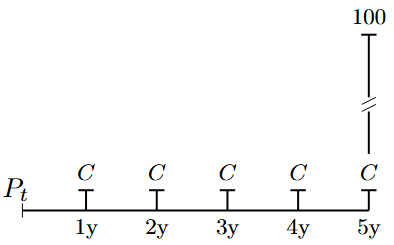
\includegraphics[keepaspectratio]{img/BondCF1.png}}

}

\caption{\label{fig-bond-cf-1}Cash flows of a \(5\)y, fixed coupon bond,
with annual coupon payments}

\end{figure}%

\emph{The figure shows the stylised payments associated with a
fixed-coupon paying bond. In this example, an annual coupon frequency is
used. The coupon payments are denoted by \(C\), and the face (notional)
value is \(100\) EUR.}

\begin{figure}

\centering{

\pandocbounded{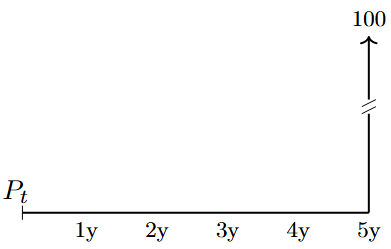
\includegraphics[keepaspectratio]{img/BondCF2.png}}

}

\caption{\label{fig-bond-cf-2}Cashflows of \(5\)y, zero-coupon}

\end{figure}%

\emph{The figure shows the stylised payments associated with a
zero-coupon bond, i.e.~a bond that does not pay any coupons during its
lifetime. The notional value is \(100\) EUR.}

\begin{figure}

\centering{

\pandocbounded{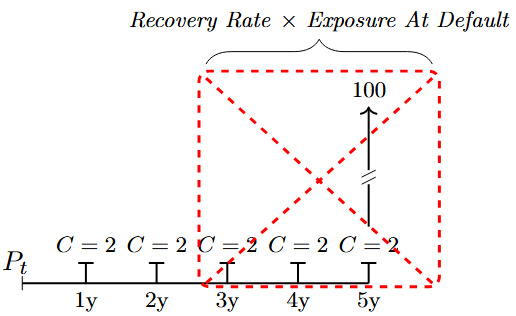
\includegraphics[keepaspectratio]{img/BondCF3.png}}

}

\caption{\label{fig-bond-cf-3}Cash flows of a defaulting \(5\)y, fixed
coupon bond, with annual coupon payments}

\end{figure}%

\emph{The figure shows the stylised payments associated with a
fixed-coupon paying bond. In this example, an annual coupon frequency is
used. The coupons are denoted by \(C\), and the notional value is
\(100\) EUR. The issuer of the bond defaults between year \(2\) and year
\(3\), and the cash flows that are due after the date of default will
not be paid to the bond holder; these foregone cash flows are marked in
the red box. Instead, the bond holder enters into the bankruptcy
proceedings and recovers \(RR\%\) of the exposure at default (EAD).
\textit{RR} is the recovery rate; sometimes \textit{loss given default}
(LGD) is used: \(RR=1-LGD\).}

A bond is a marketable debt security. An investor who buys a bond at
issuance (when it is first offered for sale in the market) effectively
extends a loan to the issuer. However, the investor does not need to
hold the bond until it matured. At any time, the bond can be sold to
another investor, either on the organised securities exchange where it
is listed, or over the counter (i.e.~outside a formal exchange). The
ease and speed with which an investor can find a willing counterparty
depend on how attractive the bond is, i.e.~how liquid it is. Highly
liquid bonds trade readily, whereas less liquid bonds are more difficult
to buy or sell.

\section*{Money market instruments}\label{money-market-instruments}
\addcontentsline{toc}{section}{Money market instruments}

\markright{Money market instruments}

The money market makes up the short-maturity end of the bond market:
instruments having maturities less than one year, at the time of
issuance, is typically categorised as belonging to the money market.
This market clears the short term borrowing and lending needs of banks
and companies.

From a monetary policy perspective, the money market constitutes the
traditional transmission channel for ECB's policy.\footnote{Jean‑Claude
  Trichet served as President of the ECB from November 1, 2003, to
  October 31, 2011.} By requiring banks to hold deposits with the ECB,
via the minimum reserve requirements, a liquidity deficit is created at
the aggregate level, and banks therefore need to borrow from each other,
and ultimately from the ECB. By steering the rate at which banks borrow
funds at, at the ECB, the short term (one-weeks) interest rate is under
the control of the ECB and steered for policy purposes. In fact, the ECB
sets three key interest rates:

\begin{itemize}
\tightlist
\item
  The policy rate (mentioned above), also called the rate on the main
  refinancing operations (MRO rate), is the rate that the ECB charges to
  the banks who obtain fund in these weekly operations. Banks have to
  provide the ECB with security in the form of collateral when obtaining
  funding.
\item
  The deposit facility rate, is the rate afforded to banks if they place
  funds in overnight deposits with the ECB. This rate is lower than the
  MRO rate.
\item
  The marginal lending facility rate, is the rate charged to the banks
  who need overnight credit; for example, if they were not able to
  obtain funding from other banks. This rate is above the MRO rate.
\end{itemize}

Short term lending and borrowing is of course also taking place directly
between banks; this \emph{interbank market} is enveloped by the deposit
facility and the rate on the marginal lending facility. These two rates
define a corridor for the interbank overnight-market rate, where the
deposit facility rate acts as the floor and the marginal lending
facility acts as the ceiling.

Collateralised lending performed by the ECB takes the form of
reverse-repurchase agreements. A repurchase agreement (repo) is an
product where the initiator exchanges collateral (bonds and other
eligible assets) for liquidity (i.e.~for a loan); a reverse-repo is the
same operation, but seen from the perspective of the party that issues
the loan (and thus receives the collateral). Therefore, the traditional
liquidity providing operations of the ECB are reverse repos: the ECB
receives collateral in exchange for loans given to banks
(counterparties).

The money markets are relevant for other ECB activities as well. In the
management of the own funds and the foreign reserve portfolios,
liquidity from maturing instruments and received coupon payments need to
be place until they can be reinvested at the next monthly rebalancing
dates. The instruments typically used for these purposes are:

\protect\phantomsection\label{tab:MoneyMarketInstruments}
\begin{longtable}[]{@{}ll@{}}
\caption{Money Market Instruments}\tabularnewline
\toprule\noalign{}
Instrument & Comment \\
\midrule\noalign{}
\endfirsthead
\toprule\noalign{}
Instrument & Comment \\
\midrule\noalign{}
\endhead
\bottomrule\noalign{}
\endlastfoot
Central Bank Deposit & Although generally restricted, other central
banks and Commercial and other eligible banks can place deposits with
the domestic central bank, typically at rates that are lower than
comparable market rates \\
Government Bills & Are tradable instruments with a maturity up to one
year, issued by a sovereign \\
Deposits & Excess cash can be placed with counterparties, as unsecured
deposits whereby a fixed or variable rate is earned during the time the
cash is placed with the counterparty \\
Repos & Excess cash can be placed with a counterparty via a repo, this
gives safety to the depositor against the default of the counterparty
via the collateral embedded in the repo transaction \\
FIXBIS & Are tradable fixed-rate instruments issued by the Bank for
International Settlements (BIS), that are available for maturities
between one week and one year, and that can be bought by central banks
and official international institutions \\
\end{longtable}

\bookmarksetup{startatroot}

\chapter{Bond Prices and Yields}\label{bond-prices-and-yields}

In equilibrium, all asset prices are determined by a common pricing
mechanism that values future payoffs after adjusting for their risk.
Following , the fundamental pricing relation is:
\begin{equation}\protect\phantomsection\label{eq-fundamentalPrice}{  
\begin{align}
    P_t = \mathbb{E}_t\!\left( \mathcal{M}_{t+1} x_{t+1}\right),
\end{align}
}\end{equation}

where \(x_{t+1}\) denotes the payoff (cash flow) at time \(t+1\), and
\(\mathcal{M}_{t+1}\) is the (stochastic) risk‑adjusted discount factor,
which can vary over time. Although Equation~\ref{eq-fundamentalPrice} is
written for a single period, it extends to multiple periods by applying
it iteratively. For example, the price at time \(t\) of a standard
\(T\)-period coupon bond with coupon \(C\) each period and notional
\(N\) at maturity, can be written as
\begin{equation}\protect\phantomsection\label{eq-gen-0026}{  
\begin{align}
P_t 
  &= \mathbb{E}_t\!\left( \mathcal{M}_{t+1} C 
    + \mathcal{M}_{t+2} C 
    + \cdots 
    + \mathcal{M}_{t+T} (C + N) \right) \\
  &= \mathbb{E}_t\!\left( \sum_{j=1}^{T} \mathcal{M}_{t+j} \, x_{t+j} \right),
\end{align}
}\end{equation}

where \(x_{t+j} = C\) for \(j=(1,\ldots,T-1)\) and \(x_{t+T} = C+N\).
The bond price therefore equals the conditional expectation of the sum
of all future cash flows, each multiplied by the appropriate
time-specific discount factor.

Applied to a credit-risk free (default free) coupon paying bond, the
pricing equation becomes:

\begin{tcolorbox}[enhanced jigsaw, arc=.35mm, bottomrule=.15mm, bottomtitle=1mm, breakable, colback=white, colbacktitle=quarto-callout-note-color!10!white, colframe=quarto-callout-note-color-frame, coltitle=black, left=2mm, leftrule=.75mm, opacityback=0, opacitybacktitle=0.6, rightrule=.15mm, title=\textcolor{quarto-callout-note-color}{\faInfo}\hspace{0.5em}{Note}, titlerule=0mm, toprule=.15mm, toptitle=1mm]

\begin{equation}\protect\phantomsection\label{eq-gen-0027}{  
\begin{align}
P_t = \sum_{j=1}^{N} \left(1 + y_{t+j}\Delta \right)^{\,-(j-1+w)} x_j,
\end{align}
}\end{equation}

\(y_t\) denotes the annualised \(t\)-specific yield (in decimals), \(m\)
is the number of coupon payments per year, implying that
\(\Delta =\dfrac{1}{m}\), \(x_j\) denotes the \(j\)th cash flow, \(N\)
is the number of remaining cash flows, and \(w \in (0,1]\) is the
fraction of the current coupon period from the settlement date to the
next coupon date, and
\begin{equation}\protect\phantomsection\label{eq-gen-0028}{  
\begin{align}
 \mathcal{M}_{t+j} = \left(1 + y_{t+j}\Delta \right)^{\,-(j-1+w)}
\end{align}
}\end{equation}

is the corresponding (discrete-time) discount factor.

\end{tcolorbox}

\begin{tcolorbox}[enhanced jigsaw, arc=.35mm, bottomrule=.15mm, bottomtitle=1mm, breakable, colback=white, colbacktitle=quarto-callout-note-color!10!white, colframe=quarto-callout-note-color-frame, coltitle=black, left=2mm, leftrule=.75mm, opacityback=0, opacitybacktitle=0.6, rightrule=.15mm, title=\textcolor{quarto-callout-note-color}{\faInfo}\hspace{0.5em}{Note}, titlerule=0mm, toprule=.15mm, toptitle=1mm]

\begin{equation}\protect\phantomsection\label{eq-gen-0029}{  
\begin{align}
P_t &= \sum_{j=1}^{N} e^{-y_{t+j}\,\tau_{t,j}}\,x_j,
\end{align}
}\end{equation}

where \(y_{t+j}\) denotes the continuously compounded yield (in
decimals) applicable to the \(j\)th cash flow, \(\tau_{t,j}\) is the
(year-fraction) time from settlement \(t\) to the payment date of cash
flow \(x_j\), \(N\) is the number of remaining cash flows, and
\begin{equation}\protect\phantomsection\label{eq-gen-0030}{  
\begin{align}
\mathcal{M}_{t+j} = e^{-y_{t+j}\,\tau_{t,j}}
\end{align}
}\end{equation}

is the corresponding (continuous-time) discount factor.

\end{tcolorbox}

\section{Bond characteristics}\label{subsec:bondCharacteristics}

Lets start with an example to frame ideas. Say today is 17 February
2026, and we sample the most liquid US government bonds from Bloomberg
by choosing ISINs that have more than USD 60 bn outstanding, a maturity
between \(10\) days and 15 years form now, fixed coupons, bullet
repayment (i.e.~that the principal is repaid in full at the maturity of
the bond), and a Bloomberg liquidity score of \(100\%\). This results in
122 bonds that are stored in the Excel file named
"Liquid\_US\_Bonds.xlsx". To illustrate, Table~\ref{tbl-bonds} shows 3
of these bonds.

\begin{longtable}[]{@{}llll@{}}
\caption{US Treasury bonds on \(17\) February
2026}\label{tbl-bonds}\tabularnewline
\toprule\noalign{}
\endfirsthead
\endhead
\bottomrule\noalign{}
\endlastfoot
ISIN & US91282CKY65 & US91282CMV09 & US91282CGQ87 \\
Amount Outstanding (USD bn) & 69.717 & 70.776 & 119.635 \\
Liquidity Score & 100 & 100 & 100 \\
Coupon & 4.625 & 3.875 & 4 \\
Coupon Type & FIXED & FIXED & FIXED \\
Coupons per year & 2 & 2 & 2 \\
Dirty/Clean price & CLEAN & CLEAN & CLEAN \\
Last Price (clean) & 100.38 & 100.47 & 101.80 \\
Bid Price (clean) & 100.32 & 100.42 & 101.75 \\
Ask Price (clean) & 100.43 & 100.46 & 101.79 \\
Accrued Interest & 0.63 & 1.50 & 1.89 \\
Bid Price (dirty) & 100.95 & 101.93 & 103.63 \\
Ask Price (dirty) & 101.04 & 101.97 & 103.68 \\
Issue date & 01/07/2024 & 31/03/2025 & 28/02/2023 \\
Maturity date & 30/06/2026 & 31/03/2027 & 28/02/2030 \\
Security Type & US GOVT & US GOVT & US GOV \\
Bullet payment & Y & Y & Y \\
Day count convention & ACT/ACT & ACT/ACT & ACT/ACT \\
Par amount (USD) & 100 & 100 & 100 \\
\end{longtable}

The entries in Table~\ref{tbl-bonds} are briefly described below:

\begin{itemize}
\tightlist
\item
  ISIN: International Securities Identification Number that uniquely
  identifies each bond.
\item
  Amount Outstanding (USD bn): Total nominal value of the bond issue
  currently in the market, measured in billions of US dollars.
\item
  Liquidity Score: Indicator of how easily the bond can be traded
  without moving the price (higher values typically mean better
  liquidity, depending on the vendor scale).
\item
  Coupon: Annual coupon rate in percent, i.e.~the yearly interest
  payment as a percentage of face value.
\item
  Coupon Type: Specifies whether the coupon is fixed, floating, or
  another structure; here all bonds have a fixed coupon.
\item
  Coupons per year: Number of coupon payments made per year (e.g.~2 for
  semi‑annual payments).
\item
  Dirty/Clean price: Indicates whether the quoted price is a clean price
  (excluding accrued interest) or a dirty price (including accrued
  interest).
\item
  Last Price: Most recent traded or quoted clean price of the bond.
\item
  Bid Price: Price at which dealers are willing to buy the bond (clean
  price).
\item
  Ask Price: Price at which dealers are willing to sell the bond (clean
  price).
\item
  Accrued Interest: Interest that has accumulated since the last coupon
  payment, payable by the buyer to the seller on settlement.
\item
  Bid Price (Dirty): Bid price including accrued interest, i.e.~the full
  amount a seller would receive per 100 of face value.
\item
  Ask Price (Dirty): Ask price including accrued interest, i.e.~the full
  amount a buyer would pay per 100 of face value.
\item
  Issue date: Date on which the bond was first issued and began accruing
  interest.
\item
  Maturity date: Date on which the bond principal is scheduled to be
  repaid and regular coupon payments stop.
\item
  Security Type: Classification of the instrument; here it denotes that
  these are US government securities.
\item
  Bullet payment: Indicates that the principal is repaid in a single
  lump sum at maturity (no amortisation).
\item
  Day count convention: Rule (e.g.~ACT/ACT) used to compute year
  fractions for interest accrual and yield calculations.
\item
  Par Amount: Nominal principal value of the bond that will be repaid at
  maturity, and on which coupon payments are calculated (typically 100
  or 1,000 per bond, independent of its market price).
\end{itemize}

As an example consider the bond in the last column of
Table~\ref{tbl-bonds}. This bons has semi-annual coupon payments, the
annual coupon rate is \(4\%\) so the size of the semi-annual coupons is
USD \(2.00\), given that the par amount is USD \(100\). The bond
specific cash flows are shown in Figure~\ref{fig-bondexample}.

\begin{figure}

\centering{

\pandocbounded{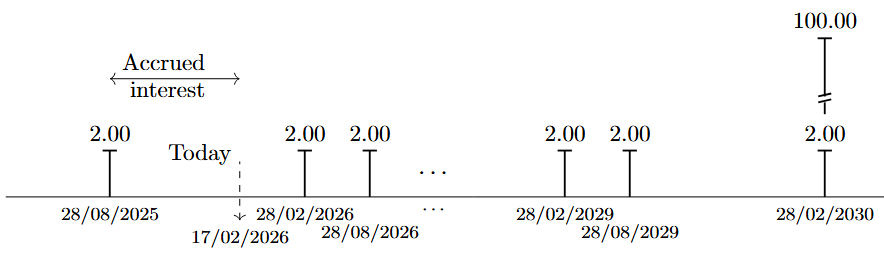
\includegraphics[keepaspectratio]{img/BondExample.png}}

}

\caption{\label{fig-bondexample}Cash flows of US91282CGQ87, annual
coupon 4\%, semi annual payments, and face value of USD 100}

\end{figure}%

The date of \(17\) February 2026 is marked as "today". Say we hold the
depicted bond and we want to sell it today, and that the prices referred
in Table Table~\ref{tbl-bonds} represent actual tradeable market prices.
Since we want to sell the bond, the relevant price is the clean bid
price, \(P_{bid,clean}=101.75\). When trading government bonds in the US
market, the bond and the payment changes hands \(1\) day after the trade
is agreed upon. This is "called settlement at \(T+1\)". The accrued
interest corresponds to the proportion of the coming coupon payment (on
\(28\) February \(2026\)) that has been earned so far, i.e.~since the
last coupon payment on \(28\) August \(2025\). To calculate the relevant
fraction it is observed that the day count convention is ACT/ACT which
means that the actual number of calendar days are use (other conventions
are e.g.~ACT/360 and ACT/365). Hence, there are \(173\) days from last
coupon payment to \(17\) February \(2026\), so the fraction of the
coming coupon that we have earned by holding the bond until now is:
\(173/365 \cdot 4\% \cdot USD 100=USD 1.89\). This means that on the
settlement day, we will receive:
\(P_{bid,clean}+\text{Accrued Interest}=103.63=P_{bid,dirty}\).

Figure~\ref{fig-bondexample} also shows that if we are interested in
calculating the yield-to-maturity of a bond, it is the dirty price that
should be matched up with the cash flows. The dirty price is the
economic value of the bond at settlement, and this is precisely what we
obtain when we calculate the present value of the future expected cash
flows. Although this point is standard in practice, it is not always
made explicit in textbooks and online resources.

The yield-to-maturity is defined as the single discount rate that
equates the present value of all remaining cash flows to the price of
the bond on the settlement date. When we discount the future cash flows
back to the settlement date (here 18/02/2026, i.e.~\(T+1\)), the
resulting present value naturally includes compensation for the interest
that has accrued since the last coupon date (28/08/2025). In other
words, the discounting operation is agnostic to any split between
``clean'' and ``accrued'': it simply collapses every future cash flow
into a single lump-sum value as of today. That lump sum is, by
construction, the dirty price (also called the invoice or full price),
i.e.~the amount of money that actually changes hands at settlement. The
relationship between the bond price and the yield-to-maturity is given
by:

\begin{tcolorbox}[enhanced jigsaw, arc=.35mm, bottomrule=.15mm, bottomtitle=1mm, breakable, colback=white, colbacktitle=quarto-callout-note-color!10!white, colframe=quarto-callout-note-color-frame, coltitle=black, left=2mm, leftrule=.75mm, opacityback=0, opacitybacktitle=0.6, rightrule=.15mm, title=\textcolor{quarto-callout-note-color}{\faInfo}\hspace{0.5em}{Note}, titlerule=0mm, toprule=.15mm, toptitle=1mm]

\protect\phantomsection\label{eqn:ytm}{}
\begin{equation}\protect\phantomsection\label{eq-ytm}{  
\begin{align}
        P_{dirty} = \sum_{j=1}^{N} \left(1 + ytm\Delta \right)^{\,j-1+w} x_j,
\end{align}
}\end{equation}

where \(ytm\) is the annualised yield-to-maturity (with \(m\) coupon
payments per year, and \(\Delta =\dfrac{1}{m}\)), \(x_j\) denotes the
\(j\)th future cash flow, \(N\) is the number of remaining cash flows,
and \(w \in (0,1]\) is the fraction of the current coupon period from
the settlement date to the next coupon date.

\end{tcolorbox}

It is important to recognise that the \(ytm\) is derived from the price
of the bond and from the future cash flows; it is not metric that, as
such, is fundamental to the bond. If the price changes, the \(ytm\)
changes - not the other way around.

It is shown in the accompanying MATLAB live script how an iterative
technique can be used to find the yield-to-maturity for the bond with
ISIN: US91282CGQ87, and how MATLAB's build in function can be used to
find the yield-to-maturity for all the sampled US government bonds. The
result for ISIN: US91282CGQ87 is \(3.53\%\) using the home-composed
iterative approach, and \(3.57\%\) using MATLABs bndyield function
(which also relies on an iterative approach) - the difference of 4 bps
is well within the uncertainty that is embedded in the data, e.g.~when
in the day the observations are recorded.

\section{Yield curves}\label{yield-curves}

The yield curve is a fundamental object in fixed income and
macro‑financial analysis. It summarises the relationship between
interest rates (or bond yields) and their time to maturity for a given
currency and credit quality, and thus provides a term structure of
discount rates for valuing cash flows across horizons.

In practice, the yield curve is used extensively for pricing. It helps
identify mispriced securities relative to a benchmark term structure,
provides valuation inputs for assets that trade infrequently, and
underpins the setting of lending rates by banks on products such as
mortgages and corporate loans through appropriate spreads over the
relevant benchmark curve.

The yield curve also plays a central role in economic and policy
analysis. Because bond prices and yields embed market participants'
expectations about future short‑term interest rates, inflation and
growth, as well as risk premia, the shape and dynamics of the curve
convey information about the expected future path of monetary policy and
the broader macroeconomic outlook. For this reason, policymakers,
investors and researchers closely monitor changes in the slope and
curvature of the yield curve as high‑frequency indicators of evolving
economic conditions.

\begin{tcolorbox}[enhanced jigsaw, arc=.35mm, bottomrule=.15mm, bottomtitle=1mm, breakable, colback=white, colbacktitle=quarto-callout-note-color!10!white, colframe=quarto-callout-note-color-frame, coltitle=black, left=2mm, leftrule=.75mm, opacityback=0, opacitybacktitle=0.6, rightrule=.15mm, title=\textcolor{quarto-callout-note-color}{\faInfo}\hspace{0.5em}{Note}, titlerule=0mm, toprule=.15mm, toptitle=1mm]

The yield curve is a graphical representation of how the yield to
maturity on comparable bonds vary with their time to maturity.

\end{tcolorbox}

Starting with the yield-to-maturity of the \(122\) liquid US bonds
introduced above, e Figure~\ref{fig-yields-ytm} shows the resulting
relationship between \(ytm\) and the maturity date of each bond in the
data sample. Each bond's \(ytm\) is marked by a yellow dot, while the
blue line in the figure is the yield curve estimated by Bloomberg for
the same day. This is the so‑called zero‑coupon yield curve (or spot
rate curve), which shows the yield on hypothetical default‑free
zero‑coupon bonds, at standard maturities \(n\in\{3,12,24,\ldots,120\}\)
months.

\begin{figure}

\centering{

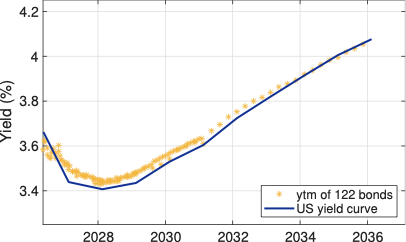
\includegraphics[width=0.85\linewidth,height=\textheight,keepaspectratio]{img/yields_ytm.png}

}

\caption{\label{fig-yields-ytm}US yield curve and \(ytm\) of 122 US
bonds on 17-Feb-2026}

\end{figure}%

As shown in (Equation~\ref{eq-ytm}), the yield‑to‑maturity of a coupon
bond is the single discount rate that makes the present value of all
promised cash flows (coupons plus principal) exactly equal to the
observed (dirty) market price; it is therefore the rate of return earned
by an investor who buys the bond at this price and holds it to maturity,
assuming all payments are made as scheduled and can be reinvested at the
same rate. As a concept, \(ytm\) is identical to the internal rate of
return familiar from microeconomics and corporate‑finance textbooks.
Because the actual market discounting is done with maturity‑specific
zero‑coupon (spot) rates, the \(ytm\) can be interpreted as a
cash‑flow‑weighted average of these underlying spot rates. It follows
that \(ytm\) will lie above the zero‑coupon yield curve when the spot
curve is downward sloping, and below it when the spot curve is
monotonically upward sloping.

Zero‑coupon yields themselves are directly linked to the stochastic
discount factors that price default‑free government bonds: for each
maturity, the zero‑coupon price is the conditional expectation of the
corresponding discount factor, and the associated spot rate is the
continuously (or discretely) compounded return that equates this price.
In this sense, the zero‑coupon yield curve summarises how the market
discounts risk‑adjusted future pay‑offs at different horizons, and
serves as the basic building block on top of which various term premia
and credit‑risk premia are added to price other fixed‑income
instruments, equities, and derivatives.

Another concept is the par yield curve. For each maturity it shows the
yield‑to‑maturity on a hypothetical bond that trades exactly at its par
value, i.e.~where the present value of all coupon and principal payments
equals the bond's face value rather than its (dirty) market price as in
(Equation~\ref{eq-ytm}). The par yield curve therefore traces the
maturity dependent coupon rates consistent with par pricing. It is
therefore particularly relevant for bond issuers, who are primarily
interested in the coupon (and thus average funding cost) that the market
is willing to support for new issuance at different tenors. From the
viewpoint of a financial analyst focused on valuation and risk, however,
the par curve is mainly a convenient way to summarise issuance
conditions and market borrowing costs at standard maturities, rather
than a primary object of analysis.

By contrast, the zero‑coupon yield curve is the fundamental object for
in fixed‑income analysis. It is the spot curve that enters no‑arbitrage
valuation formulas, underlies the extraction of forward rates, and
provides the natural platform for modelling term premia and other risk
adjustments that connect observed bond prices to expectations about
future short‑term interest rates and macroeconomic developments.

In practice the zero‑coupon yield curve itself is not directly
observable, because most government bonds pay coupons. Instead, it is
estimated from traded bond prices. There are basically two ways to do
this: (1) bootstrapping, and (2) functional approaches.

\subsection{Bootstrapping the zero-coupon
curve}\label{bootstrapping-the-zero-coupon-curve}

Bootstrapping proceeds recursively from the shortest to the longest
maturity. For example, using the bonds sampled on \(17\)-FEB-\(2026\)
the cross‑section of prices and coupons are directly observed. Let
\({P^{(k)}_t}\) be the price for the \(k=\{1,2,\ldots,K\}\) bonds, where
\(K=122\) for our sample, coupon rates are denoted by \({c^{(k)}}\), and
maturities by \({T^{(k)}}\). For the shortest‑maturity bond, which has
only a single cash flow at \(T^{(1)}\), the spot rate \(s_{t+1}\) is
found directly from the standard pricing equation:

\begin{equation}\protect\phantomsection\label{eq-gen-0032}{  
\begin{align}
    P^{(1)}_t = \frac{1 + c^{(1)}\Delta}{\bigl(1+s_{t+1}\Delta\bigr)^{1}} .
\end{align}
}\end{equation}

For the next bond in the maturity ordering, the price equation involves
both the already‑identified short‑maturity discount factor and the
unknown discount factor at the new maturity. Proceeding like this, the
price of bond \(k\) can be written as:
\begin{equation}\protect\phantomsection\label{eq-gen-0033}{  
\begin{align}
    P^{(k)}_t &= \sum_{j=1}^{N^{(k)}-1} \frac{c^{(k)}\Delta}{\bigl(1+s_{t+j}\Delta\bigr)^{j}}
    + \frac{1 + c^{(k)}\Delta} {\bigl(1+s_{t+N^{(k)}}\Delta\bigr)^{N^{(k)}}},
\end{align}
}\end{equation}

with all discount factors up to maturity \(T^{(k-1)}\) are already known
from earlier steps, so this equation can be solved for the new spot rate
\(s_{t+N^{(k)}}\) at maturity \(T^{(k)}\).

Repeating this forward‑substitution step across the ordered set of bond
maturities yields a full discrete set of zero‑coupon yields.

\begin{tcolorbox}[enhanced jigsaw, arc=.35mm, bottomrule=.15mm, bottomtitle=1mm, breakable, colback=white, colbacktitle=quarto-callout-note-color!10!white, colframe=quarto-callout-note-color-frame, coltitle=black, left=2mm, leftrule=.75mm, opacityback=0, opacitybacktitle=0.6, rightrule=.15mm, title=\textcolor{quarto-callout-note-color}{\faInfo}\hspace{0.5em}{Note}, titlerule=0mm, toprule=.15mm, toptitle=1mm]

\textbf{Input:} Prices \(P_t^{(k)}\), coupons \(c^{(k)}\), maturities
\(T^{(k)}\), common coupon interval \(\Delta\), ordered so that
\(T^{(1)}<T^{(2)}<\dots<T^{(K)}\).

\textbf{Step 1 (shortest maturity).} If bond \(1\) has only one cash
flow at \(T^{(1)}\), solve
\begin{equation}\protect\phantomsection\label{eq-gen-0034}{  
\begin{align}
    P_t^{(1)}  &= \frac{1 + c^{(1)}\Delta}{\bigl(1+s_{t+1}\Delta\bigr)}
\end{align}
}\end{equation}

for the first spot rate \(s_{t+1}\).

\textbf{Step 2 (for \(k=2,\dots,K\)).} For bond \(k\) with
\(N^{(k)} = T^{(k)}/\Delta\) coupon dates, write its price as
\begin{equation}\protect\phantomsection\label{eq-gen-0035}{  
\begin{align}
    P_t^{(k)}
      &= \sum_{j=1}^{N^{(k)}-1} 
          \frac{c^{(k)}\Delta}{\bigl(1+s_{t+j}\Delta\bigr)^{j}}
          + \frac{1 + c^{(k)}\Delta}
                 {\bigl(1+s_{t+N^{(k)}}\Delta\bigr)^{N^{(k)}}}.
\end{align}
}\end{equation}

All spot rates \(s_{t+1},\dots,s_{t+N^{(k)}-1}\) are known from earlier
steps, so this equation can be solved for the new spot rate
\(s_{t+N^{(k)}}\).

\end{tcolorbox}

MATLAB provides a built‑in routine in the Econometrics Toolbox,
\(zbtprice\), which implements the bootstrapping procedure for coupon
bonds. The accompanying MATLAB live script illustrates how this function
is applied to the US Treasury sample, and the resulting zero‑coupon
yield curve is reported in Figure~\ref{fig-yields-ytm-zcc} alongside the
curves already shown in Figure~\ref{fig-yields-ytm} for comparison.

\begin{figure}

\centering{

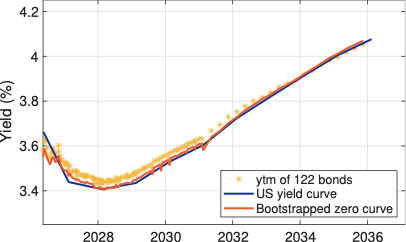
\includegraphics[width=0.85\linewidth,height=\textheight,keepaspectratio]{img/yields_ytm_zcc.png}

}

\caption{\label{fig-yields-ytm-zcc}Zero-coupon yield curve extracted
from the 122 US bonds on 17-Feb-2026}

\end{figure}%

Because of the sequential design of the bootstrapping technique, each
bond's contribution to the zero-curve is unique and the resulting zero
coupon curve will therefore reflect any idiosyncrasies pertaining to the
bonds in the sample. This is seen in the curve by its jagged movements
through-out the maturity spectrum.

Because the bootstrap procedure constructs discount factors
sequentially, each bond affects a distinct segment of the term
structure, and the calculated zero‑coupon curve inevitably inherits any
bond‑specific noise or illiquidity effects. This is visible in
Figure~\ref{fig-yields-ytm-zcc} as small, jagged oscillations of the
curve across maturities, rather than a perfectly smooth profile.

In an arbitrage‑free market, zero‑coupon rates for nearby maturities
should evolve smoothly, since they are all derived from trading the same
underlying risk‑free asset over only slightly different horizons.
Pronounced kinks or local reversals in the zero‑coupon curve signal that
some bonds are priced inconsistently with others, so that appropriately
designed long--short portfolios could, at least in principle, exploit
these discrepancies by borrowing at relatively ``cheap'' maturities and
lending at relatively ``expensive'' ones.\footnote{In the affine
  term-structure literature there are two common, but equivalent, sign
  conventions. Some authors (e.g.~Joslin, Singleton and Zhu) define bond
  prices as \(P_t^{(n)} = \exp(A_n + B_n^\top X_t)\), which implies
  \(y_t^{(n)} = -\tfrac{1}{n}(A_n + B_n^\top X_t)\) and hence
  \(a_n = -A_n/n\), \(b_n = -B_n/n\). Here, we instead start from the
  pricing relation
  \(P_t^{(n)} = \exp\!\big(-\sum_{j=0}^{(n-1)} r_{t+j}\Delta t\big)\)
  and use the definition \(y=-\tfrac{1}{n}log(P)\), such that
  \(E_t(y_t^{(n)}) = \tfrac{1}{n}E_t(A_n + B_n^\top X_t)\) and
  \(a_n = A_n/n\), \(b_n = B_n/n\). Both conventions are algebraically
  equivalent; only the placement of the minus sign differs.} The jagged
behaviour in Figure~\ref{fig-yields-ytm-zcc} therefore represents
bond‑specific noise and market frictions embedded in the observed
prices. To avoid such undesirable curve features, a functional form for
the zero-curve can be imposed.

\subsection{Parametric Estimation of the Zero‑Coupon Yield
Curve}\label{parametric-estimation-of-the-zerocoupon-yield-curve}

Typical parametric specifications used to impose a smoothness on the
zero‑coupon spot rate include:

\begin{itemize}
\tightlist
\item
  Nelson-Siegel:
\item
  Svensson-Soderlind:
\item
  Splines: and
\end{itemize}

The Nelson-Siegel model uses \(4\) parameters,
\(\theta_{NS}=\{ \beta_0, \beta_1, \beta_2, \lambda\}\) and specifies
the continuously compounded spot rate as:
\begin{equation}\protect\phantomsection\label{eq-gen-0036}{  
\begin{align}
    z_{NS}(n) = \beta_0 + \beta_1 \left(\frac{1-e^{-\lambda n}}{\lambda n}\right) + \beta_2 \left(\frac{1-e^{-\lambda n}}{\lambda n} - e^{-\lambda n}\right).
\end{align}
}\end{equation}

In the original formulation the exponential term is written as
\(e^{-n/\tau}\); here \(\lambda = 1/\tau\) is used for notational
convenience. The Svensson-Soderlind model extends the Nelson-Siegel
model with an additional curvature term, uses \(6\) parameters,
\(\theta_{SS}=\{ \beta_0, \beta_1, \beta_2, \beta_3, \lambda_1, \lambda_2\}\),
and is given by:
\begin{equation}\protect\phantomsection\label{eq-gen-0037}{ 
\begin{align}
    z_{SS}(n) = \beta_0 + \beta_1 \left(\frac{1-e^{-\lambda_1 n}}{\lambda_1 n}\right) &+& \beta_2 \left(\frac{1-e^{-\lambda_1 n}}{\lambda_1 n} - e^{-\lambda_1 n}\right) \nonumber \\
    &+& \beta_3 \left(\frac{1-e^{-\lambda_2 n}}{\lambda_2 n} - e^{-\lambda_2 n}\right)
\end{align}
}\end{equation}

Both models are built from a small set of generic yield‑curve
components. The parameter \(\beta_0\) governs the long‑run level of the
curve: changing \(\beta_0\) shifts the entire zero‑coupon term structure
up or down, and with only \(\beta_0\) active the curve would be flat
across all maturities, moving only in parallel. The parameter
\(\beta_1\) controls (minus) the slope of the curve, mainly affecting
short maturities relative to the long end, while \(\beta_2\) and, in the
Svensson--Söderlind extension, \(\beta_3\) introduce one or two
curvature components that allow for humps or troughs at intermediate
maturities. The maturity‑dependent functions multiplying these
parameters (the loading functions) are plotted in
Figure~\ref{fig-NN-SS-loadings}; they can be interpreted as the
sensitivity of the spot rate at each maturity to a marginal change in
the corresponding parameter.

\begin{figure}

\centering{

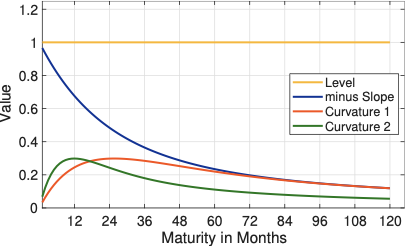
\includegraphics[width=0.85\linewidth,height=\textheight,keepaspectratio]{img/NS_SS_loadings.png}

}

\caption{\label{fig-NN-SS-loadings}Nelson-Siegel and Svensson-Soderlind
loading functions}

\end{figure}%

Spline methods approximate the zero‑coupon curve by combining basis
functions, for example low‑degree polynomials, across maturity segments,
while enforcing smoothness where the segments meet. To illustrate, a
cubic spline defined a set of knot maturities
\(0<\kappa_1<\dots<\kappa_J\) leads to this functional form for the
discount function \(D(n)\):
\begin{equation}\protect\phantomsection\label{eq-gen-0038}{  
\begin{align}
    D(n) = \alpha_0 + \alpha_1 n + \alpha_2 n^2 + \alpha_3 n^3
    + \sum_{j=1}^{J} \gamma_j (n-\kappa_j)_+^3,
\end{align}
}\end{equation}

where \((\cdot)_+ = \max\{\cdot,0\}\) and the coefficients
\(\theta_{Cspline}=\{\alpha_0,\alpha_1,\alpha_2,\alpha_3,\gamma_j\}\)
are estimated from the available bond prices. The zero‑coupon
(continuously compounded) spot rate then follows from the definition
\begin{equation}\protect\phantomsection\label{eq-gen-0039}{  
\begin{align}
z_{\texttt{spline}}(n)
= -\frac{1}{n}\log\left[ D(n) \right]
= -\frac{1}{n}\log\!\left[
\alpha_0 + \alpha_1 n + \alpha_2 n^2 + \alpha_3 n^3
+ \sum_{j=1}^{J} \gamma_j (n-\kappa_j)_+^3
\right].
\end{align}
}\end{equation}

The three first terms of the discount function are active across all
maturities, while each cubic basis function \((n-\kappa_j)_+^3\) is zero
before its knot and then gradually ``switches on'' after \(\kappa_j\),
so adjusting \(\gamma_j\) affects the local shape of the curve beyond
that maturity without affecting shorter maturities. By estimating the
coefficients to fit observed bond prices (often with an additional
smoothness penalty), spline‑based methods balance cross‑sectional fit
and smoothness: they can track complex term‑structure shapes more
closely than parsimonious models such as Nelson--Siegel and
Svensson-Soderlind, at the cost of estimating a larger number of
parameters and choosing knot locations.

Intuitively, fitting a spline model to the zero‑coupon curve can be
viewed as walking along the maturity spectrum and, at each step,
layering maturity‑specific behaviour extracted from observed bond prices
on top of an underlying global polynomial of chosen order; in the
example above, this baseline is a cubic (third‑degree) polynomial.

Another important distinction between parametric and spline‑based models
concerns their alignment with financial theory. A central tenet is
internal model consistency, in the sense that the model explicitly rules
out arbitrage opportunities in line with equation
Equation~\ref{eq-fundamentalPrice}, i.e.~that it implies a unique
stochastic discount factor. Nelson--Siegel type models satisfy this
requirement for all practical purposes,\footnote{This is an example of
  the general idea of certainty-equivalent cash flows: the risk
  adjustment is moved into the pricing kernel (or, equivalently, into
  the probability measure under which prices are computed), so that the
  resulting cash flows can be discounted at the risk-free rate. More
  broadly, it reflects the fundamental principle that the riskiness of
  cash flows and the discount rate must be aligned.} whereas
spline‑based specifications are essentially statistical devices that
balance flexibility of the functional form against cross‑sectional fit.
If the observed bond prices are themselves arbitrage‑free, then a spline
fitted to those prices will inherit the no‑arbitrage property at the
calibrated point in time, but this is a consequence of the data rather
than a structural feature of the model. In equilibrium, this would
implicitly require that prices are determined by traders using
internally consistent valuation models, while the spline user is merely
a marginal observer of those prices. In that sense, spline‑based
term‑structure models are descriptive rather than structural and are
not, by themselves, natural candidates for modelling equilibrium
pricing.

The accompanying MATLAB live script demonstrates how the Nelson--Siegel,
Svensson--Soderlind, and spline‑based frameworks can be implemented in
practice using the sample of \(122\) US government bonds.

\begin{figure}

\centering{

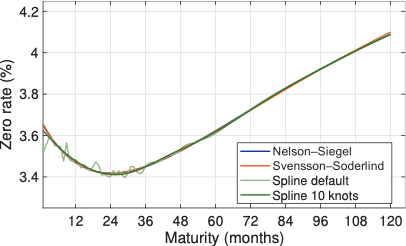
\includegraphics[width=0.85\linewidth,height=\textheight,keepaspectratio]{img/zc_NS_SS_Spline.png}

}

\caption{\label{fig-zc-NS-SS-Spline}Fitted cero-coupon yield curves on
17-Feb-2026}

\end{figure}%

\begin{tcolorbox}[enhanced jigsaw, arc=.35mm, bottomrule=.15mm, bottomtitle=1mm, breakable, colback=white, colbacktitle=quarto-callout-note-color!10!white, colframe=quarto-callout-note-color-frame, coltitle=black, left=2mm, leftrule=.75mm, opacityback=0, opacitybacktitle=0.6, rightrule=.15mm, title=\textcolor{quarto-callout-note-color}{\faInfo}\hspace{0.5em}{Note}, titlerule=0mm, toprule=.15mm, toptitle=1mm]

Input: Observed bond prices \(P_t^{(k)}\), coupons \(c^{(k)}\),
maturities \(T^{(k)}\), common coupon interval \(\Delta\),
\(k=1,\dots,K\). Choose a parametric specification for the spot rate
curve, \(s\), at maturity \(n\):
\begin{equation}\protect\phantomsection\label{eq-gen-0040}{  
\begin{align}
      s(n;\theta) = s\big(n;\theta_1,\dots,\theta_M\big),
\end{align}
}\end{equation}

with parameter vector \(\theta = (\theta_1,\dots,\theta_M)^{\top}\) of
dimension \(M \ll K\).

\textbf{Step 1 (discount factors implied by the spot curve).} Given
\(\theta\), the discount factor for maturity \(n\) is:
\begin{equation}\protect\phantomsection\label{eq-gen-0041}{  
\begin{align}
      D(n;\theta) = \exp\!\left(-n\,s(n;\theta)\right),
\end{align}
}\end{equation}

For bond \(k\) with coupon dates \(T^{(k)}_j = j\Delta\) and
\(N^{(k)} = T^{(k)}/\Delta\) payments, the model price is:
\begin{equation}\protect\phantomsection\label{eq-gen-0042}{  
\begin{align}
      P^{(k)}_{\text{model}}(\theta)
      = \sum_{j=1}^{N^{(k)}} c^{(k)}\Delta\,D(T^{(k)}_j;\theta)
      + 100 \cdot D(T^{(k)};\theta),
\end{align}
}\end{equation}

\textbf{Step 2 (parameter estimation).} Choose \(\theta\) to make model
prices as close as possible to observed prices. A standard choice is the
least-squares criterion, possibly including weights, \(w_k\):
\begin{equation}\protect\phantomsection\label{eq-gen-0043}{  
\begin{align}
      \widehat{\theta}
      = \arg\min_{\theta} \sum_{k=1}^{K} w_k  \big(P_t^{(k)} - P^{(k)}_{\text{model}}(\theta)\big)^2,
\end{align}
}\end{equation}

where \(w_k\) are user-chosen weights (for example based on duration or
liquidity).

\textbf{Output (fitted zero-coupon curve).} The estimated parameter
vector \(\widehat{\theta}\) defines a smooth spot-rate function
\(s(n;\widehat{\theta})\).

\end{tcolorbox}

Figure~\ref{fig-zc-NS-SS-Spline} plots zero‑coupon yield curves
estimated on 17 February 2026 using three different approaches: the
parametric Nelson--Siegel and Svensson--Soderlind specifications, and
two spline‑based curves. The MATLAB default spline fit produces a very
flexible curve that closely tracks short‑maturity quotation noise and
displays several small oscillations in the 6--36 month segment,
illustrating how a highly parameterised spline can overfit idiosyncratic
features of the data. When the spline is restricted to only \(10\) knot
points, the fitted curve becomes much smoother and its shape essentially
coincides with that of the Nelson--Siegel and Svensson--Soderlind
term‑structure models over the entire maturity range. This highlights a
certain degree of arbitrariness and data dependence inherent in
spline‑based yield‑curve estimation: changing the knot structure, while
leaving the underlying bond prices unchanged, can lead to noticeably
different zero‑coupon curves at the short end, whereas more parsimonious
specifications deliver shapes that are much closer to those implied by
standard parametric models.

\bookmarksetup{startatroot}

\chapter{Matrix Algebra}\label{matrix-algebra}

The objective of this section is to give a concise overview of how
matrix operations can be applied to solve financial problems and models
of relevance for the material presented in this book. A more
comprehensive and detailed treatment of matrix algebra can be found, for
example, in The Matrix Cookbook ().\footnote{Formally, this term ensures
  that, after the change of measure to \(\mathbb{Q}\), discounted asset
  prices are martingales.}

\section{Vectors and matrices}\label{vectors-and-matrices}

A column vector is an ordered collection of numbers written vertically
as \begin{equation}\protect\phantomsection\label{eq-gen-0044}{  
\begin{align}
    \mathbf{x} = \begin{bmatrix}
        x_{1} \\ x_{2} \\ \vdots \\ x_{k}
\end{bmatrix},
\end{align}
}\end{equation}

where \(x_{j} \in \mathbb{R}\) denotes the \(j\)th element and \(k\) is
the dimension of the vector.

A row vector is written horizontally as
\begin{equation}\protect\phantomsection\label{eq-gen-0045}{  
\begin{align}
    \mathbf{x}^{\top} = \begin{bmatrix}
    x_{1} & x_{2} & \cdots & x_{k}
\end{bmatrix}.
\end{align}
}\end{equation}

An \(m \times k\) matrix \(\mathbf{A}\) is a rectangular array of
numbers with \(m\) rows and \(k\) columns,
\begin{equation}\protect\phantomsection\label{eq-gen-0046}{  
\begin{align}
\mathbf{A}
=
\begin{bmatrix}
a_{11} & a_{12} & \cdots & a_{1k} \\
a_{21} & a_{22} & \cdots & a_{2k} \\
\vdots & \vdots & \ddots & \vdots \\
a_{m1} & a_{m2} & \cdots & a_{mk}
\end{bmatrix}.
\end{align}
}\end{equation}

The element in row \(i\) and column \(j\) is denoted \(a_{ij}\). Square
matrices have \(m = k\).

\section{Transpose}\label{transpose}

The transpose of an \(m \times k\) matrix \(\mathbf{A}\) is the
\(k \times m\) matrix obtained by turning rows into columns,
\begin{equation}\protect\phantomsection\label{eq-gen-0047}{ 
\begin{align}
\mathbf{A}^{\top}
=
\begin{bmatrix}
a_{11} & a_{21} & \cdots & a_{m1} \\
a_{12} & a_{22} & \cdots & a_{m2} \\
\vdots & \vdots & \ddots & \vdots \\
a_{1k} & a_{2k} & \cdots & a_{mk}
\end{bmatrix}.
\end{align}
}\end{equation}

For vectors this implies that the transpose of a column vector is a row
vector and vice versa.

Transposition is linear and reverses the order of matrix products:
\begin{equation}\protect\phantomsection\label{eq-gen-0048}{  
\begin{align}
(\mathbf{A} + \mathbf{B})^{\top} &= \mathbf{A}^{\top} + \mathbf{B}^{\top}, \\
(c\,\mathbf{A})^{\top}           &= c\,\mathbf{A}^{\top}, \\
(\mathbf{A}\mathbf{B})^{\top}    &= \mathbf{B}^{\top}\mathbf{A}^{\top}, \\
(\mathbf{A}\mathbf{B}\mathbf{C})^{\top}
                                   &= \mathbf{C}^{\top}\mathbf{B}^{\top}\mathbf{A}^{\top},
\end{align}
}\end{equation}

whenever the products are well defined and \(c\) is a scalar.

\section{Matrix multiplication}\label{matrix-multiplication}

If \(\mathbf{A}\) is \(m \times k\) and \(\mathbf{B}\) is
\(k \times r\), then the product \(\mathbf{C}=\mathbf{A}\mathbf{B}\) is
the \(m \times r\) matrix with elements
\begin{equation}\protect\phantomsection\label{eq-gen-0049}{  
\begin{align}
c_{ij} = \sum_{\ell=1}^{k} a_{i\ell} b_{\ell j}.
\end{align}
}\end{equation}

In finance this operation appears, for example, when computing the
values of several portfolios from a vector of asset prices and a matrix
of portfolio weights.

Matrix multiplication is associative and distributive, but not
commutative in general:
\begin{equation}\protect\phantomsection\label{eq-gen-0050}{  
\begin{align}
\mathbf{A}(\mathbf{B}\mathbf{C}) &= (\mathbf{A}\mathbf{B})\mathbf{C}, \\
\mathbf{A}(\mathbf{B}+\mathbf{C}) &= \mathbf{A}\mathbf{B} + \mathbf{A}\mathbf{C}, \\
\mathbf{A}\mathbf{B} &\neq \mathbf{B}\mathbf{A} \quad \text{in general}.
\end{align}
}\end{equation}

\section{Identity matrix and inverse}\label{identity-matrix-and-inverse}

The \(k \times k\) identity matrix, denoted \(\mathbf{I}_{k}\) or simply
\(\mathbf{I}\), has ones on the diagonal and zeros elsewhere,
\begin{equation}\protect\phantomsection\label{eq-gen-0051}{  
\begin{align}
\mathbf{I}_{k}
=
\begin{bmatrix}
1 & 0 & \cdots & 0 \\
0 & 1 & \cdots & 0 \\
\vdots & \vdots & \ddots & \vdots \\
0 & 0 & \cdots & 1
\end{bmatrix}.
\end{align}
}\end{equation}

It acts as a multiplicative neutral element:
\(\mathbf{I}_{k}\mathbf{A}=\mathbf{A}\) and
\(\mathbf{A}\mathbf{I}_{k}=\mathbf{A}\) whenever the products are
defined.

A square matrix \(\mathbf{A}\) is invertible (or nonsingular) if there
exists a matrix \(\mathbf{A}^{-1}\) such that
\begin{equation}\protect\phantomsection\label{eq-gen-0052}{  
\begin{align}
\mathbf{A}^{-1}\mathbf{A} = \mathbf{I}
\quad\text{and}\quad
\mathbf{A}\mathbf{A}^{-1} = \mathbf{I}.
\end{align}
}\end{equation}

The matrix \(\mathbf{A}^{-1}\) is called the inverse of \(\mathbf{A}\).

A necessary and sufficient condition for a square matrix to be
invertible is that its determinant is non‑zero. Equivalently, the
columns (or rows) of \(\mathbf{A}\) must be linearly independent. In
terms of linear systems, \(\mathbf{A}\) is invertible if and only if the
system \begin{equation}\protect\phantomsection\label{eq-gen-0053}{  
\begin{align}
\mathbf{A}\mathbf{x} = \mathbf{b}
\end{align}
}\end{equation}

has a unique solution \(\mathbf{x}\) for every right‑hand side
\(\mathbf{b}\).

Inverse and transpose interact with products in a way that mirrors the
rules for scalars:
\begin{equation}\protect\phantomsection\label{eq-gen-0054}{  
\begin{align}
(\mathbf{A}\mathbf{B})^{-1} &= \mathbf{B}^{-1}\mathbf{A}^{-1},
\quad\text{if $\mathbf{A}$ and $\mathbf{B}$ are invertible}, \\
(\mathbf{A}^{\top})^{-1} &= (\mathbf{A}^{-1})^{\top},
\quad\text{if $\mathbf{A}$ is invertible}.
\end{align}
}\end{equation}

\section{Eigenvalue decomposition}\label{eigenvalue-decomposition}

The eigenvalue decomposition of a matrix is closely related to principal
component analysis (PCA). In financial modelling, PCA is often used to
reduce the dimensionality of complex datasets, helping to summarise
large amounts of information with a few key components. This aligns with
many financial models, which seek to explain observable variables
through a small number of underlying drivers; for example, the Capital
Asset Pricing Model (CAPM) assumes that equity returns are primarily
driven by a single market factor, and dynamic yield-curve models
typically assume that movements in the term structure of interest rates
can be well approximated by a few latent factors, often interpreted as
level, slope, and curvature.

Let \(\mathbf{S}\) be a symmetric positive semi-definite \(k\times k\)
matrix, for example a covariance matrix. Its eigenvalue decomposition is
\begin{equation}\protect\phantomsection\label{eq-gen-0055}{  
\begin{align}
    \mathbf{S} = \mathbf{L}\mathbf{D}\mathbf{L}^{-1} = \mathbf{L}\mathbf{D}\mathbf{L}^{\top},
\end{align}
}\end{equation}

where the second equality uses the fact that the columns of
\(\mathbf{L}\) form an orthonormal set, such that
\begin{equation}\protect\phantomsection\label{eq-gen-0056}{  
\begin{align}
    \mathbf{L}^{\top}\mathbf{L} = \mathbf{I}_k \quad \Leftrightarrow \quad \mathbf{L}^{-1} = \mathbf{L}^{\top}.
\end{align}
}\end{equation}

Here \(\mathbf{L}\) is a \(k\times k\) matrix collecting the
eigenvectors as columns, and \(\mathbf{D}\) is a \(k\times k\) diagonal
matrix containing the corresponding eigenvalues.

Now let \(\mathbf{Y}\) be a \(T\times k\) time-series data matrix, with
each column representing a variable and each row a time observation.
Projecting \(\mathbf{Y}\) onto the eigenvectors yields the time series
of principal components:
\begin{equation}\protect\phantomsection\label{eq-gen-0057}{  
\begin{align}
    \mathbf{Y} = \mathbf{F}\mathbf{L}^{\top},
\end{align}
}\end{equation}

where \(\mathbf{F}\) is a \(T\times k\) matrix of factor scores
(principal components). Because \(\mathbf{L}\) is orthonormal, this can
be viewed as a linear regression of \(\mathbf{Y}\) on the loadings
\(\mathbf{L}\); the least-squares estimator of \(\mathbf{F}\) is
\begin{equation}\protect\phantomsection\label{eq-gen-0058}{  
\begin{align}
    \hat{\mathbf{F}} 
    = \mathbf{Y}\mathbf{L}\left(\mathbf{L}^{\top}\mathbf{L}\right)^{-1} 
    = \mathbf{Y}\mathbf{L},
\end{align}
}\end{equation}

using \(\mathbf{L}^{\top}\mathbf{L} = \mathbf{I}_k\). Substituting back
gives the exact reconstruction
\begin{equation}\protect\phantomsection\label{eq-gen-0059}{  
\begin{align}
    \mathbf{Y} = \hat{\mathbf{F}}\mathbf{L}^{\top}.
\end{align}
}\end{equation}

To reduce the data dimensionality, order the eigenvalues in
\(\mathbf{D}\) from largest to smallest and partition
\begin{equation}\protect\phantomsection\label{eq-gen-0060}{  
\begin{align}
    \mathbf{L} = \left[\;\mathbf{L}_{1:l}\ \ \mathbf{L}_{l+1:k}\;\right], 
    \quad
    \hat{\mathbf{F}} = \left[\;\hat{\mathbf{F}}_{1:l}\ \ \hat{\mathbf{F}}_{l+1:k}\;\right],
\end{align}
}\end{equation}

where \(\mathbf{L}_{1:l}\) is \(k\times l\) and
\(\hat{\mathbf{F}}_{1:l}\) is \(T\times l\). The exact decomposition can
then be written as
\begin{equation}\protect\phantomsection\label{eq-gen-0061}{  
\begin{align}
    \mathbf{Y} = \hat{\mathbf{F}}_{1:l}\mathbf{L}_{1:l}^{\top} 
      \;+\; \hat{\mathbf{F}}_{l+1:k}\mathbf{L}_{l+1:k}^{\top}.
\end{align}
}\end{equation}

Dimensionality reduction is achieved by retaining only the first \(l<k\)
components and discarding the remainder. In that case, \(\mathbf{Y}\) is
approximated as
\begin{equation}\protect\phantomsection\label{eq-gen-0062}{  
\begin{align}
    \mathbf{Y} \approx \hat{\mathbf{F}}_{1:l}\mathbf{L}_{1:l}^{\top},
\end{align}
}\end{equation}

or, equivalently,
\begin{equation}\protect\phantomsection\label{eq-gen-0063}{  
\begin{align}
    \mathbf{Y} = \hat{\mathbf{F}}_{1:l}\mathbf{L}_{1:l}^{\top} + \mathbf{E},
\end{align}
}\end{equation}

where \(\mathbf{E}\) is a \(T\times k\) approximation error capturing
the contribution of the discarded components.

\section{Matrix rotation}\label{matrix-rotation}

Consider a nonsingular matrix \(\mathbf{R}\) that satisfies
\begin{equation}\protect\phantomsection\label{eq-gen-0064}{  
\begin{align}
    \mathbf{I} = \mathbf{R}^{-1} \mathbf{R}.
\end{align}
}\end{equation}

The matrix \(\mathbf{R}\) can be interpreted as a rotation matrix that
can alter the orientation of factors, e.g.~extracted using principal
component analysis, without changing the overall explanatory content of
a model. Starting from the generic factor representation:
\begin{equation}\protect\phantomsection\label{eq-gen-0065}{  
\begin{align}
    \mathbf{Y} &= \mathbf{F} \, \mathbf{L}^{\top} + \mathbf{E} \nonumber \\
    &= \mathbf{F} \, \mathbf{I} \, \mathbf{L}^{\top} + \mathbf{E} \nonumber \\
    &= \mathbf{F} \, \mathbf{R}^{-1}\mathbf{R} \,\mathbf{L}^{\top} + \mathbf{E} \nonumber \\   
    &= \underbrace{\mathbf{F} \, \mathbf{R}^{-1}}_{\tilde{\mathbf{F}}}
        \underbrace{(\mathbf{R} \, \mathbf{L}^{\top})}_{\tilde{\mathbf{L}}^{\top}} + \mathbf{E}
\end{align}
}\end{equation}

gives the rotated representation:
\begin{equation}\protect\phantomsection\label{eq-gen-0066}{  
\begin{align}
    \mathbf{Y} = \tilde{\mathbf{F}}\, \tilde{\mathbf{L}}^{\top} + \mathbf{E},
\end{align}
}\end{equation}

where \(\tilde{\mathbf{F}} = \mathbf{F}\mathbf{R}^{-1}\) and
\(\tilde{\mathbf{L}}^{\top} = \mathbf{R}\mathbf{L}^{\top}\) are rotated
versions of \(\mathbf{F}\) and \(\mathbf{L}^{\top}\), respectively.

This transformation leaves the fitted values \(\mathbf{Y}\) unchanged
but redistributes the variation among the factors and loadings.

\bookmarksetup{startatroot}

\chapter{The normal distribution, value at Risk, and expected
Shortfall}\label{the-normal-distribution-value-at-risk-and-expected-shortfall}

In many applications in finance, (log-)returns on assets or portfolios
are modelled using the normal distribution. Let \(x\) denote the
(random) portfolio return over a fixed horizon, and assume that
\begin{equation}\protect\phantomsection\label{eq-gen-0067}{  
\begin{align}
    x \sim N(m,\sigma^{2}),
\end{align}
}\end{equation}

where \(m\) is the mean return and \(\sigma>0\) is the standard
deviation (volatility) of returns.

\subsection*{Quantiles of the normal
distribution}\label{quantiles-of-the-normal-distribution}
\addcontentsline{toc}{subsection}{Quantiles of the normal distribution}

For a given probability level \(0<\alpha<1\), the \(\alpha\)--quantile
of \(x\) is the value \(q_{\alpha}\) such that
\begin{equation}\protect\phantomsection\label{eq-gen-0068}{  
\begin{align}
    \mathbb{P}(x \leq q_{\alpha}) = \alpha.
\end{align}
}\end{equation}

If \(\Phi(\cdot)\) denotes the cumulative distribution function (cdf) of
a standard normal variable \(z\sim N(0,1)\), then the
\(\alpha\)--quantile of \(x\) has the closed form:
\begin{equation}\protect\phantomsection\label{eq-gen-0069}{  
\begin{align}
    q_{\alpha} = m + \sigma\,\Phi^{-1}(\alpha)
\end{align}
}\end{equation}

where \(\Phi^{-1}(\cdot)\) is the quantile function of the standard
normal distribution.

\subsection*{Value at Risk}\label{value-at-risk}
\addcontentsline{toc}{subsection}{Value at Risk}

Value at Risk (VaR) is a widely used summary measure of downside risk.
For a given confidence level \(0<\alpha<1\), the \(\alpha\)--level VaR
is the loss threshold that will not be exceeded with probability
\(\alpha\) over the given horizon. If we work with returns and define
losses as \(L=-X\), the VaR at level \(\alpha\) is the
\(\alpha\)--quantile of \(L\),
\begin{equation}\protect\phantomsection\label{eq-gen-0070}{  
\begin{align}
    \mathrm{VaR}_{\alpha} &= q^{L}_{\alpha} \\
                          &= -\mu + \sigma\,\Phi^{-1}(\alpha),
\end{align}
}\end{equation}

because \(L=-X \sim \mathcal{N}(-\mu,\sigma^{2})\) has quantiles
\(q^{L}_{\alpha}=-\mu+\sigma\Phi^{-1}(\alpha)\). Equivalently, in
return-space one may express the VaR as the negative of a low return
quantile, \begin{equation}\protect\phantomsection\label{eq-gen-0071}{ 
\begin{align}
    \mathrm{VaR}_{\alpha} = -q^{X}_{1-\alpha}
                         = -\mu + \sigma\,\Phi^{-1}(1-\alpha),
\end{align}
}\end{equation}

corresponding, for example, to the \(1\%\) worst daily return at a
\(99\%\) confidence level.

\subsection*{Expected Shortfall}\label{expected-shortfall}
\addcontentsline{toc}{subsection}{Expected Shortfall}

Expected Shortfall (ES), also known as Tail Conditional Expectation or
Conditional Value at Risk, refines VaR by taking into account not only
the quantile at the VaR level, but also the average size of losses
beyond this threshold. For the loss variable \(L=-X\), the Expected
Shortfall at level \(\alpha\) is defined as
\begin{equation}\protect\phantomsection\label{eq-gen-0072}{  
\begin{align}
    \mathrm{ES}_{\alpha}  &= \mathbb{E}\big[L \;\big|\; L \geq \mathrm{VaR}_{\alpha}\big],
\end{align}
}\end{equation}

that is, the conditional expectation of the loss, given that it lies in
the worst \((1-\alpha)\) fraction of the loss distribution.

Under the normality assumption \(X\sim\mathcal{N}(\mu,\sigma^{2})\) and
hence \(L=-X\sim\mathcal{N}(-\mu,\sigma^{2})\), the Expected Shortfall
has a closed form. Let \(z_{\alpha}=\Phi^{-1}(\alpha)\) denote the
standard normal \(\alpha\)--quantile, and let \(\varphi(\cdot)\) denote
the standard normal density. Then
\begin{equation}\protect\phantomsection\label{eq-gen-0073}{ 
\begin{align}
    \mathrm{VaR}_{\alpha} &= -\mu + \sigma\,z_{\alpha}, \\
    \mathrm{ES}_{\alpha}  &= -\mu + \sigma\,\frac{\varphi(z_{\alpha})}{1-\alpha},
\end{align}
}\end{equation}

so that the Expected Shortfall exceeds the VaR by an amount proportional
to the normal density evaluated at the VaR quantile.

These expressions are often referred to as ``parametric'' or
``delta--normal'' formulas for VaR and Expected Shortfall, and are
widely used in practice when the normality assumption for (linear)
portfolios is judged to be a reasonable approximation.

\begin{longtable}[]{@{}lccc@{}}
\caption{Scaling factors for VaR and ES based from the Normal
distribution}\tabularnewline
\toprule\noalign{}
\endfirsthead
\endhead
\bottomrule\noalign{}
\endlastfoot
Confidence level & Tail probability & VaR multiplier & ES multiplier \\
\(\alpha\) & \(1-\alpha\) & \(z_{\alpha}\) &
\(\dfrac{\varphi(z_{\alpha})}{1-\alpha}\) \\
90\% & 10\% & 1.2816 & 1.755 \\
95\% & 5\% & 1.6449 & 2.062 \\
97.5\% & 2.5\% & 1.9600 & 2.338 \\
99\% & 1\% & 2.3263 & 2.665 \\
99.5\% & 0.5\% & 2.5758 & 2.917 \\
99.9\% & 0.1\% & 3.0902 & 3.372 \\
\end{longtable}

\bookmarksetup{startatroot}

\chapter{Covariance and Correlation}\label{sec:cov_corr}

When modelling asset returns it is rarely enough to know the risk of
each asset in isolation. What matters for portfolios is how returns move
together. This co-movement is summarised by covariance and correlation.

Let \(x\) and \(y\) denote two random variables, for example one-period
returns on two assets, with means \(m_x = \mathbb{E}(x)\) and
\(m_y = \mathbb{E}(y)\). Their covariance is defined as
\begin{equation}\protect\phantomsection\label{eq-gen-0074}{  
\begin{align}
    \mathrm{Cov}(x,y)  = \mathbb{E}\big[(x - m_x)(y - m_y)\big].
\end{align}
}\end{equation}

A positive covariance means that \(x\) and \(y\) tend to be above or
below their means at the same time; a negative covariance means that
when one is above its mean, the other tends to be below its mean. The
variance is the special case \(\mathrm{Var}(x) = \mathrm{Cov}(x,x)\).

In empirical work we observe a time series \(\{x_t,y_t\}_{t=1}^T\) and
estimate the mean, variance, and covariance from the data. An estimator
of the covariance is
\begin{equation}\protect\phantomsection\label{eq-covar}{  
\begin{align}
    \widehat{\mathrm{Cov}}(x,y)
    &= \frac{1}{T-1} \sum_{t=1}^T
        \big(x_t - \bar{x}\big)\big(y_t - \bar{y}\big),
\end{align}
}\end{equation}

where \begin{equation}\protect\phantomsection\label{eq-gen-0076}{  
\begin{align}
    \bar{x} = \frac{1}{T}\sum_{t=1}^T x_t,
    \qquad
    \bar{y} = \frac{1}{T}\sum_{t=1}^T y_t.
\end{align}
}\end{equation}

The corresponding sample variances are obtained by setting \(x=y\) in
Equation~\ref{eq-covar}.

\section*{Covariance matrices}\label{covariance-matrices}
\addcontentsline{toc}{section}{Covariance matrices}

\markright{Covariance matrices}

For a \(k\)-dimensional random vector of returns
\begin{equation}\protect\phantomsection\label{eq-gen-0077}{ 
\begin{align}
    \mathbf{x}_t
    &=
    \begin{bmatrix}
        x_{1t} \\ x_{2t} \\ \vdots \\ x_{kt}
    \end{bmatrix},
\end{align}
}\end{equation}

the variance and covariances can be collected in the \(k\times k\)
covariance matrix
\begin{equation}\protect\phantomsection\label{eq-gen-0078}{  
\begin{align}
    \Sigma
    &= \mathrm{Var}(\mathbf{x}_t)
     \;=\; \mathbb{E}\big[(\mathbf{x}_t - \mathbf{m})
                         (\mathbf{x}_t - \mathbf{m})^{\top}\big],
\end{align}
}\end{equation}

where \(\mathbf{m} = \mathbb{E}(\mathbf{x}_t)\). The diagonal elements
of \(\Sigma\) are the variances of each return series and the
off-diagonal elements are their covariances. In sample, with
observations \(\{\mathbf{x}_t\}_{t=1}^T\) and sample mean
\(\bar{\mathbf{x}} = T^{-1}\sum_{t=1}^T \mathbf{x}_t\), a standard
estimator is
\begin{equation}\protect\phantomsection\label{eq-gen-0079}{  
\begin{align}
    \hat{\Sigma}
    &= \frac{1}{T-1} \sum_{t=1}^T
        (\mathbf{x}_t - \bar{\mathbf{x}})
        (\mathbf{x}_t - \bar{\mathbf{x}})^{\top}.
\end{align}
}\end{equation}

This matrix will play a central role in portfolio analysis, where the
variance of a portfolio with weight vector \(\mathbf{w}\) is given by
\(\sigma_p^2 = \mathbf{w}^{\top} \Sigma \mathbf{w}\); this will be
studied in detail in the dedicated portfolio-optimisation chapter.

\section*{Correlation and the correlation
matrix}\label{correlation-and-the-correlation-matrix}
\addcontentsline{toc}{section}{Correlation and the correlation matrix}

\markright{Correlation and the correlation matrix}

While covariance measures joint variability in the units of the
variables themselves, correlation is a unit-free measure that normalises
by the standard deviations. The correlation between \(x\) and \(y\) is
\begin{equation}\protect\phantomsection\label{eq-gen-0080}{  
\begin{align}
    \rho_{x,y}
    &= \frac{\mathrm{Cov}(x,y)}
             {\sqrt{\mathrm{Var}(x)}\sqrt{\mathrm{Var}(y)}}.
\end{align}
}\end{equation}

By construction, \(\rho_{x,y} \in [-1,1]\): values near \(1\) indicate
strong positive co-movement, values near \(-1\) indicate strong negative
co-movement, and values near \(0\) indicate weak linear dependence.

For a \(k\)-dimensional return vector, the pairwise correlations can be
collected in the \(k\times k\) correlation matrix \(R\), whose
\((i,j)\)th element is
\begin{equation}\protect\phantomsection\label{eq-gen-0081}{  
\begin{align}
    R_{ij}
    &= \frac{\Sigma_{ij}}
             {\sqrt{\Sigma_{ii}}\,\sqrt{\Sigma_{jj}}}.
\end{align}
}\end{equation}

Equivalently, if \(D\) is the diagonal matrix of standard deviations,
\(D = \mathrm{diag}(\sqrt{\Sigma_{11}},\ldots,\sqrt{\Sigma_{kk}})\),
then \begin{equation}\protect\phantomsection\label{eq-gen-0082}{  
\begin{align}
    R &= D^{-1} \Sigma \, D^{-1}.
\end{align}
}\end{equation}

Both \(\Sigma\) and \(R\) are symmetric and positive semi-definite
matrices, and both will be used repeatedly in what follows when
modelling returns, measuring risk, and constructing optimal portfolios.

\begin{tcolorbox}[enhanced jigsaw, arc=.35mm, bottomrule=.15mm, bottomtitle=1mm, breakable, colback=white, colbacktitle=quarto-callout-note-color!10!white, colframe=quarto-callout-note-color-frame, coltitle=black, left=2mm, leftrule=.75mm, opacityback=0, opacitybacktitle=0.6, rightrule=.15mm, title=\textcolor{quarto-callout-note-color}{\faInfo}\hspace{0.5em}{Note}, titlerule=0mm, toprule=.15mm, toptitle=1mm]

For random variables \(x\) and \(y\) with means \(m_x\) and \(m_y\), the
covariance and correlation are
\begin{equation}\protect\phantomsection\label{eq-gen-0083}{  
\begin{align}
    \mathrm{Cov}(x,y)
    &= \mathbb{E}\big[(x - m_x)(y - m_y)\big],\\
    \rho_{x,y}
    &= \frac{\mathrm{Cov}(x,y)}
             {\sqrt{\mathrm{Var}(x)}\sqrt{\mathrm{Var}(y)}}.
\end{align}
}\end{equation}

For a \(k\)-dimensional return vector with covariance matrix \(\Sigma\),
the correlation matrix \(R\) has elements
\begin{equation}\protect\phantomsection\label{eq-gen-0084}{  
\begin{align}
    R_{ij} &= \frac{\Sigma_{ij}}
                    {\sqrt{\Sigma_{ii}}\,\sqrt{\Sigma_{jj}}}.
\end{align}
}\end{equation}

\end{tcolorbox}

\section*{Expectations and
covariances}\label{expectations-and-covariances}
\addcontentsline{toc}{section}{Expectations and covariances}

\markright{Expectations and covariances}

In asset pricing we are often interested in finding the expectation to a
product of random variables, for example in the context of the SDF in
Equation~\ref{eq-fundamentalPrice}. If \(x\) and \(y\) are two random
variables, then the expectation of their product can be expressed as:

\begin{tcolorbox}[enhanced jigsaw, arc=.35mm, bottomrule=.15mm, bottomtitle=1mm, breakable, colback=white, colbacktitle=quarto-callout-note-color!10!white, colframe=quarto-callout-note-color-frame, coltitle=black, left=2mm, leftrule=.75mm, opacityback=0, opacitybacktitle=0.6, rightrule=.15mm, title=\textcolor{quarto-callout-note-color}{\faInfo}\hspace{0.5em}{Note}, titlerule=0mm, toprule=.15mm, toptitle=1mm]

\begin{equation}\protect\phantomsection\label{eq-expectation-product}{
\begin{align}
    \mathbb{E}(xy) = \mathrm{Cov}(x,y) + \mathbb{E}(x)\mathbb{E}(y).
\end{align}
}\end{equation}

\end{tcolorbox}

This follows from the definition of covariance:
\begin{align}
    \mathrm{Cov}(x,y) &= \mathbb{E}\big[(x - m_x)(y - m_y)\big] \nonumber \\
                      &= \mathbb{E}\big[(xy) - x m_y - y m_x + m_x m_y \big] \nonumber \\
                      & = \mathbb{E}(xy) - m_y \mathbb{E}(x) - m_x \mathbb{E}(y) + m_x m_y \nonumber \\
                      & = \mathbb{E}(xy) - m_y m_x - m_x m_y + m_x m_y \nonumber \\
                      & = \mathbb{E}(xy) - m_x m_y \nonumber \\
                      & = \mathbb{E}(xy) - \mathbb{E}(x)\mathbb{E}(y).
\end{align}

\bookmarksetup{startatroot}

\chapter{Econometric techniques}\label{econometric-techniques}

To model dependencies between observable and unobservable variables, we
will make use of three key modelling frameworks:

\begin{itemize}
\tightlist
\item
  Linear regression
\item
  Vector autoregression of order \(p\) (VAR(\(p\))), which models the
  dynamic interactions among multiple time series
\item
  State-space models, which offer a flexible structure for representing
  systems that evolve over time and may include unobserved components
\end{itemize}

Together, these approaches provide a solid foundation for analysing both
static and dynamic relationships in economic and financial data.

\section{Linear Regression}\label{sec:linReg}

Linear regression techniques capture relationships between variables
using a simple yet powerful statistical framework. They can be applied
to time series as will as cross sectional data. Suppose we have the
linear model:
\begin{equation}\protect\phantomsection\label{eq-linear-regression}{  
\begin{align}
    \mathbf{y} = \mathbf{X}\, \hat{\beta} + \mathbf{E}
\end{align}
}\end{equation}

where \(\mathbf{y}\) is an \(m \times 1\) vector of observed dependent
variable values, \(\mathbf{X}\) is an \(m \times k\) matrix of observed
independent variable values (also called regressors or features),
\(\hat{\beta}\) is a \(k \times 1\) vector of unknown parameters to be
estimated, and \(\mathbf{E}\) is an \(m \times 1\) vector of error terms
capturing the deviation of the model from the observed data.

and we wish to estimate the unknown parameter vector \(\beta\). If
\(\mathbf{X}\) were square and invertible the solution would be:
\begin{equation}\protect\phantomsection\label{eq-gen-0086}{  
\begin{align}
    \mathbf{X}^{-1}\mathbf{y} &= \mathbf{X}^{-1}\, \mathbf{X}\, \hat{\beta} + \mathbf{X}^{-1} \mathbf{E} \nonumber \\
    \hat{\beta} &= \mathbf{X}^{-1}\mathbf{y} + \mathbf{X}^{-1} \mathbf{E}
\end{align}
}\end{equation}

However, in most applications \(\mathbf{X}\) is not square and therefore
not invertible. This is because \(\mathbf{X}\) collects the sample data
used to explain the behaviour of the variable \(y\), so its number of
rows equals the number of observations, while its number of columns
equals the number of explanatory variables (including a constant, if
present). For \(\mathbf{X}\) to be square, the number of observations
would need to be exactly equal to the number of explanatory variables,
which is rarely the case in practice.

A way to progress in then to pre-multiply
Equation~\ref{eq-linear-regression} by \(\mathbf{X}^{\top}\):
\begin{equation}\protect\phantomsection\label{eq-gen-0087}{  
\begin{align}
    \mathbf{X}^{\top}\mathbf{y} = \mathbf{X}^{\top}\mathbf{X}\, \hat{\beta} + \mathbf{X}^{\top} \mathbf{E}.
\end{align}
}\end{equation}

Now the parameter vector \(\beta\) can be found as:
\begin{equation}\protect\phantomsection\label{eq-gen-0088}{ 
\begin{align}
    \hat{\beta} &= \left(\mathbf{X}^{\top}\mathbf{X}\right)^{-1}\, \mathbf{X}^{\top}\mathbf{y}  - \left(\mathbf{X}^{\top}\mathbf{X}\right)^{-1}\mathbf{X}^{\top} \mathbf{E} \nonumber \\
    \mathbb{E}\left(\hat{\beta}\right) &= \left(\mathbf{X}^{\top}\mathbf{X}\right)^{-1}\, \mathbf{X}^{\top}\mathbf{y}.
\end{align}
}\end{equation}

Linear regression examples are included in the accompanying MATLAB live
script.

\section{Vector Autoregression}\label{vector-autoregression}

A vector autoregression (VAR) extends the univariate autoregressive, or
\(AR(p)\), model to a multivariate setting. In the univariate case, a
time series variable \(x_t\) is modelled as a linear function of its own
past values:
\begin{equation}\protect\phantomsection\label{eq-gen-0089}{ 
\begin{align}
    x_t &= c + \alpha_1 x_{t-1} + \alpha_2 x_{t-2} + \ldots + \alpha_p x_{t-p} + e_t,
\end{align}
}\end{equation}

where \(c\) is a constant term, \(\alpha_j\) are autoregressive
coefficients, and \(e_t\) is an error term assumed to be white noise.
This representation captures the dynamic dependence of \(x_t\) on its
own history.

A \emph{VAR}(\(p\)) model generalises this idea by allowing for multiple
time series. Instead of modelling a single variable, now an
\(k\)-dimensional vector of variables is modelled,
\(\mathbf{x}_t = (x_{1k}, x_{2k}, \ldots, x_{kt})^{\top}\), each
potentially depending on its own past as well as the past of all other
variables in the system. The model takes the form
\begin{equation}\protect\phantomsection\label{eq-gen-0090}{  
\begin{align}
    \mathbf{x}_t &= \mathbf{c} + \mathbf{A}_1 \mathbf{x}_{t-1} + \mathbf{A}_2 \mathbf{x}_{t-2} + \ldots + \mathbf{A}_p \mathbf{x}_{t-p} + \mathbf{e}_t,
\end{align}
}\end{equation}

where \(\mathbf{x}_t\) and \(\mathbf{c}\) are \(k \times 1\) vectors,
each \(\mathbf{A}_j\) is an \(k \times k\) coefficient matrix, and
\(\mathbf{e}_t\) is an \(k \times 1\) vector of innovations.

\subsection*{Companion form: writing a VAR(p) as a
VAR(1)}\label{companion-form-writing-a-varp-as-a-var1}
\addcontentsline{toc}{subsection}{Companion form: writing a VAR(p) as a
VAR(1)}

For many theoretical and computational purposes, it is convenient to
express any \emph{VAR}(\(p\)) model in companion form as a
\emph{VAR}(\(1\)) model. To do this, we stack current and lagged values
of \(\mathbf{x}_t\) into a single augmented state vector:
\begin{equation}\protect\phantomsection\label{eq-gen-0091}{  
\begin{align}
    \mathbf{X}_t &=
    \begin{pmatrix}
        \mathbf{x}_t \\
        \mathbf{x}_{t-1} \\
        \vdots \\
        \mathbf{x}_{t-p+1}
    \end{pmatrix},
\end{align}
}\end{equation}

which is an \(kp \times 1\) vector. The intercept and error vectors is
augmented as well:
\begin{equation}\protect\phantomsection\label{eq-gen-0092}{  
\begin{align}
    \mathbf{C} &=
    \begin{pmatrix}
        \mathbf{c} \\
        \mathbf{0} \\
        \vdots \\
        \mathbf{0}
    \end{pmatrix},
    &
    \mathbf{E}_t &=
    \begin{pmatrix}
        \mathbf{e}_t \\
        \mathbf{0} \\
        \vdots \\
        \mathbf{0}
    \end{pmatrix},
\end{align}
}\end{equation}

where \(\mathbf{0}\) denotes conformable zero vectors.

Next, we construct the \(kp \times kp\) companion matrix \(\mathbf{A}\):
\begin{equation}\protect\phantomsection\label{eq-gen-0093}{  
\begin{align}
    \mathbf{A} &=
    \begin{pmatrix}
        \mathbf{A}_1 & \mathbf{A}_2 & \cdots & \mathbf{A}_{p-1} & \mathbf{A}_p \\
        \mathbf{I}_n & \mathbf{0}   & \cdots & \mathbf{0}       & \mathbf{0}   \\
        \mathbf{0}   & \mathbf{I}_n & \cdots & \mathbf{0}       & \mathbf{0}   \\
        \vdots       & \vdots       & \ddots & \vdots           & \vdots       \\
        \mathbf{0}   & \mathbf{0}   & \cdots & \mathbf{I}_n     & \mathbf{0}
    \end{pmatrix},
\end{align}
}\end{equation}

where \(\mathbf{I}_k\) is the \(k \times k\) identity matrix.

With these definitions, the original \emph{VAR}(\(p\)) can now be
written compactly as a first-order \emph{VAR} model:
\begin{equation}\protect\phantomsection\label{eq-gen-0094}{  
\begin{align}
    \mathbf{X}_t &= \mathbf{C} + \mathbf{A}\,\mathbf{X}_{t-1} + \mathbf{E}_t.
\end{align}
}\end{equation}

This is a \emph{VAR}(\(1\)) in \(\mathbf{X}_t\), and it is
mathematically equivalent to the \emph{VAR}(\(p\)) specification for
\(\mathbf{x}_t\). The companion-form representation is particularly
useful for studying stability, since the eigenvalues of \(\mathbf{A}\)
determine whether the system is stable and stationary.

\section{Linear Gaussian State-Space Models}\label{sec:LSSM}

A state-space model consists of a state equation
Equation~\ref{eq-state-space-model}. Underlying factors are evolved in
the time series dimension via the state equation, and these state
variables are converted to observable quantities via the observation
equation. Using the notation used by MATLAB that has its origins in
control theory and early economic applications, e.g.~, , , which in
essence is also not far away from . Let \(\mathbf{x}_t\) denote an
\(k_x \times 1\) state vector, \(\mathbf{y}_t\) an \(k_y \times 1\)
vector of observed variables. A linear time-invariant state-space model
can then be written as
\begin{equation}\protect\phantomsection\label{eq-state-space-model}{  
\begin{align}
   \texttt{state eq:} \, \, \, \mathbf{x}_{t} &= \mathbf{A}\,\mathbf{x}_{t-1} + \mathbf{B}\,\mathbf{u}_t, \\
   \texttt{obs eq:} \, \, \, \mathbf{y}_t &= \mathbf{C}\,\mathbf{x}_t + \mathbf{D}\,\mathbf{e}_t, 
\end{align}
}\end{equation}

where:

\begin{itemize}
\tightlist
\item
  \(\mathbf{A}\) is the \(k_x \times k_x\) state coefficient matrix that
  governs the dynamics of the latent state.
\item
  \(\mathbf{B}\) is the \(k_x \times k_u\) state disturbance coefficient
  matrix where \(\Omega_u=\mathbf{B}\mathbf{B}^{\top}\) is the
  state-disturbance covariance matrix.
\item
  \(\mathbf{C}\) is the \(k_y \times k_x\) observation
  loading-coefficient matrix that maps states into observables.
\item
  \(\mathbf{D}\) is the \(k_y \times k_u\) observation innovation
  coefficient matrix where \(\Omega_e=\mathbf{D}\mathbf{D}^{\top}\) is
  the observation-innovation covariance matrix.
\end{itemize}

In many applications, \(\mathbf{x}_t\) can be interpreted as a
low-dimensional vector of latent factors extracted from a
higher-dimensional panel of observables \(\mathbf{y}_t\). In this case,
the columns of \(\mathbf{C}\) play the role of factor loadings, exactly
as in principal component analysis (PCA), where each observed variable
is expressed as a linear combination of a small number of principal
components.

\bookmarksetup{startatroot}

\chapter{Filters}\label{filters}

\section{The Recursive Least Squares
Filter}\label{the-recursive-least-squares-filter}

Given a linear regression model as in
Equation~\ref{eq-linear-regression}:
\begin{equation}\protect\phantomsection\label{eq-gen-0096}{  
\begin{align}
    \mathbf{y} = \mathbf{X}\, \hat{\beta} + \mathbf{E}
\end{align}
}\end{equation}

where \(\mathbf{y}=\left\{y_1, y_2, \ldots, y_k\right\}^{\top}\) is a
vector of dimension \(k \times 1\),
\(\mathbf{X}=\left\{\mathbf{x}_1, \mathbf{x}_2, \ldots, \mathbf{x}_V \right\}^{\top}\)
is a matrix of dimension \(k \times V\), where \(V\) is the number of
included explanatory variables, and
\(e=\left\{e_1, e_2, \ldots, e_k \right\}^{\top}\), is a vector of
dimension \(k \times 1\). From section \hyperref[sec:linReg]{9.1} We
have that:
\begin{equation}\protect\phantomsection\label{eq-linreg-beta}{  
\begin{align}
    \hat{\beta} = \left( \mathbf{X}^{\top} \mathbf{X}\right)^{-1} \mathbf{X}^{\top}\mathbf{y}.
\end{align}
}\end{equation}

\(\hat{\beta}\) can be re-estimated using Equation~\ref{eq-linreg-beta}
when new observations are added to \(\mathbf{y}\) and \(\mathbf{X}\).
For normal sized data this is unproblematic. However, the matrix
inversion in Equation~\ref{eq-linreg-beta} can become a computational
burden for larger datasets. This is where the Recursive Least Square
(RLS) technique becomes relevant.

Suppose an estimate \(\beta_t\) exists based on data from observation
\(1\) to \(t\). How can this estimate be updated to include this new
information without recomputing Equation~\ref{eq-linreg-beta}? First,
the new observations \(y_{z}\) (of dimension \(1 \times 1\)), and
\(\mathbf{x}_{z}\) (of dimension \(K \times 1\)) are stacked onto
\(y_t\) and \(\mathbf{x}_t\). Recall that \(y_t\) and \(\mathbf{x}_t\)
contain all observations from \(1\) to \(t\).

\begin{equation}\protect\phantomsection\label{eq-gen-0098}{  
\begin{align}
    \mathbf{y}_{t+1} = \begin{bmatrix} y_{z} \\ \mathbf{y}_t  \end{bmatrix}, \quad
    \mathbf{x}_{t+1} = \begin{bmatrix} \mathbf{x}^{\top}_{z} \\ \mathbf{X}_t  \end{bmatrix}
\end{align}
}\end{equation}

Now define: \begin{equation}\protect\phantomsection\label{eq-OLSdef}{  
\begin{align}
    S_t     &= X_t^{\top} X_t \\
    S_{t+1} &= S_t + \mathbf{x}_{z} \mathbf{x}^{\top}_{z} \\
    q_t     &= \mathbf{X}_t^{\top} \mathbf{y}_t \\
    q_{t+1} &= q_t + \mathbf{x}_{z} y_{z}.
\end{align}
}\end{equation}

The inverse \(S_t^{-1}\) can by updated using the Sherman-Morrison
formula (Sherman and Morrison 1950), which states that:
\begin{equation}\protect\phantomsection\label{eq-sherman-morrison}{  
\begin{align}
    (A + uv^T)^{-1} = A^{-1} - \frac{A^{-1} u v^T A^{-1}}{1 + v^T A^{-1} u}
\end{align}
}\end{equation}

When inserting Equation~\ref{eq-OLSdef} into
Equation~\ref{eq-sherman-morrison} we get:
\begin{equation}\protect\phantomsection\label{eq-gen-0101}{  
\begin{align}
    S_{t+1}^{-1} = S_t^{-1} - \frac{S_t^{-1} \mathbf{x}_z \mathbf{x}_z^{\top} S_t^{-1}}{1 + \mathbf{x}_z^{\top} S_t^{-1} \mathbf{x}_z}
\end{align}
}\end{equation}

and since \(\hat{\beta}_{t} = S_{t}^{-1} q_{t}\) \(\Leftrightarrow\)
\(q_{t} = S_{t} \hat{\beta}_{t}\), a recursive updating expression for
the parameter estimate \(\hat{\beta}_{t+1}\) is given by:
\begin{equation}\protect\phantomsection\label{eq-RLS}{
\begin{align}
    \hat{\beta}_{t+1} &= S_{t+1}^{-1} q_{t+1} \nonumber \\
    &= S_{t+1}^{-1} \left(q_t + \mathbf{x}_{z} y_{z} \right) \nonumber \\
    &= S_{t+1}^{-1} \left(S_{t} \hat{\beta}_{t} + \mathbf{x}_{z} y_{z} \right) \nonumber \\
    &= \left(S_t^{-1} - \frac{S_t^{-1} \mathbf{x}_z \mathbf{x}_z^{\top} S_t^{-1}} {1 + \mathbf{x}_z^{\top} S_t^{-1} \mathbf{x}_z} \right) \left(S_{t} \hat{\beta}_{t} + \mathbf{x}_{z} y_{z} \right) \nonumber \\
    &= S_t^{-1} S_{t} \hat{\beta}_{t}  
       + S_t^{-1} \mathbf{x}_{z} y_{z} 
        - \frac{S_t^{-1} \mathbf{x}_z \mathbf{x}_z^{\top} S_t^{-1}} {1 + \mathbf{x}_z^{\top} S_t^{-1} \mathbf{x}_z} S_{t} \hat{\beta}_{t}  
        -  \frac{S_t^{-1} \mathbf{x}_z \mathbf{x}_z^{\top} S_t^{-1}} {1 + \mathbf{x}_z^{\top} S_t^{-1} \mathbf{x}_z} \mathbf{x}_z y_{z} \nonumber \\
   &=  \hat{\beta}_{t} - \frac{S_t^{-1} \mathbf{x}_z } {1 + \mathbf{x}_z^{\top} S_t^{-1} \mathbf{x}_z}  \mathbf{x}_z^{\top} \hat{\beta}_{t}  
        + S_t^{-1} \mathbf{x}_z y_{z} -  \frac{S_t^{-1} \mathbf{x}_z \mathbf{x}_z^{\top} S_t^{-1}} {1 + \mathbf{x}_z^{\top} S_t^{-1} \mathbf{x}_z} \mathbf{x}_{z} y_{z} \nonumber \\
   &=  \hat{\beta}_{t} - \frac{S_t^{-1} \mathbf{x}_z } {1 + \mathbf{x}_z^{\top} S_t^{-1} \mathbf{x}_z}  \mathbf{x}_z^{\top} \hat{\beta}_{t} 
    + S_t^{-1} \mathbf{x}_{z} y_{z} \left( I - \frac{ \mathbf{x}_z^{\top} S_t^{-1} \mathbf{x}_{z} } {1 + \mathbf{x}_z^{\top} S_t^{-1} \mathbf{x}_z} \right) \nonumber \\
   &=  \hat{\beta}_{t} - \frac{S_t^{-1} \mathbf{x}_z } {1 + \mathbf{x}_z^{\top} S_t^{-1} \mathbf{x}_z}  \mathbf{x}_z^{\top} \hat{\beta}_{t} 
    + S_t^{-1} \mathbf{x}_{z} y_{z} \left( \frac{1 + \mathbf{x}_z^{\top} S_t^{-1} \mathbf{x}_z}{1 + \mathbf{x}_z^{\top} S_t^{-1} \mathbf{x}_z} - \frac{ \mathbf{x}_z^{\top} S_t^{-1} \mathbf{x}_{z} } {1 + \mathbf{x}_z^{\top} S_t^{-1} \mathbf{x}_z} \right) \nonumber \\
   &=  \hat{\beta}_{t} - \frac{S_t^{-1} \mathbf{x}_z } {1 + \mathbf{x}_z^{\top} S_t^{-1} \mathbf{x}_z}  \mathbf{x}_z^{\top} \hat{\beta}_{t} 
   +  \frac{S_t^{-1} \mathbf{x}_{z} } {1 + \mathbf{x}_z^{\top} S_t^{-1} \mathbf{x}_z} y_{z}
\end{align}
}\end{equation}

Now define: \begin{equation}\protect\phantomsection\label{eq-Krls}{  
\begin{align}
    K_{t+1} = \frac{S_t^{-1} \mathbf{x}_z}{1 + \mathbf{x}_z^{\top} S_t^{-1} \mathbf{x}_z}.
\end{align}
}\end{equation}

When Equation~\ref{eq-Krls} is inserted in Equation~\ref{eq-RLS} the
updating equation is:
\begin{equation}\protect\phantomsection\label{eq-gen-0104}{  
\begin{align}
 \nonumber
   \hat{\beta}_{t+1} &= \hat{\beta}_{t} + K_{t+1} y_n - K_{t+1} \mathbf{x}_{z}^{\top}  \hat{\beta}_{t} \\ 
   &= \hat{\beta}_{t} + K_{t+1} \left( y_z - \mathbf{x}_z^{\top} \hat{\beta}_{t} \right) 
\end{align}
}\end{equation}

This shows that \(K_{t+1}\) acts as a weighting and conversion factor:
it maps the scalar prediction error into a vector update for the
parameter estimate. The term:
\begin{equation}\protect\phantomsection\label{eq-gen-0105}{  
\begin{align}
    u_t = y_z - \mathbb{E}[y_z] = y_z - \mathbf{X}_t^{\top} \hat{\beta}_t.
\end{align}
}\end{equation}

is the one-step ahead prediction error under \(\hat{\beta}_t\). The
script called \texttt{RLS.m} implements the above described methodology
in MATLAB.

\section{The Linear Kalman Filter}\label{sec:lkf}

This section relies heavily on Hamilton (1994) and Durbin and Koopman
(2012). We consider the linear state-space model introduced in
Section~\hyperref[sec:LSSM]{9.3} (reproduced here for convenience),
Equation~\ref{eq-state-space-model}:
\begin{equation}\protect\phantomsection\label{eq-gen-0106}{ 
\begin{align}
  \mathbf{x}_{t} &= \mathbf{A}\,\mathbf{x}_{t-1} + \mathbf{B}\,\mathbf{u}_t, \\
  \mathbf{y}_{t} &= \mathbf{C}\,\mathbf{x}_{t} + \mathbf{D}\,\mathbf{e}_t. 
\end{align}
}\end{equation}

The process noise \(\mathbf{u}_t\) and the measurement noise
\(\mathbf{e}_t\) are assumed zero-mean, serially independent, and
mutually independent, with covariances
\begin{equation}\protect\phantomsection\label{eq-gen-0107}{  
\begin{align}
  \operatorname{Var}(\mathbf{u}_t) &= \mathbf{I}, &
  \operatorname{Var}(\mathbf{e}_t) &= \mathbf{I}.
\end{align}
}\end{equation}

Consequently, the process and measurement noise covariances entering the
state-space model are \(\mathbf{B}\mathbf{B}^\top\) and
\(\mathbf{D}\mathbf{D}^\top\), respectively.

Given the information set \(\mathcal{F}_{t-1}\) available up to time
\(t-1\), the state equation implies
\begin{equation}\protect\phantomsection\label{eq-gen-0108}{  
\begin{align}
  \mathbb{E}(\mathbf{x}_t \mid \mathcal{F}_{t-1})
    &= \mathbf{A}\,\mathbf{x}_{t-1\mid t-1}, \\
  \operatorname{Var}(\mathbf{x}_t \mid \mathcal{F}_{t-1})
    &= \mathbf{A}\,\mathbf{P}_{t-1\mid t-1}\,\mathbf{A}^\top
       + \mathbf{B}\,\mathbf{B}^\top.
\end{align}
}\end{equation}

Defining the predicted state and its covariance as
\begin{equation}\protect\phantomsection\label{eq-gen-0109}{  
\begin{align}
  \mathbf{x}_{t\mid t-1} &= \mathbb{E}(\mathbf{x}_t \mid \mathcal{F}_{t-1}), &
  \mathbf{P}_{t\mid t-1} &= \operatorname{Var}(\mathbf{x}_t \mid \mathcal{F}_{t-1}),
\end{align}
}\end{equation}

the prediction step of the Kalman filter can be written compactly as
\begin{equation}\protect\phantomsection\label{eq-KF-Pred}{  
\begin{align}
  \mathbf{x}_{t\mid t-1} &= \mathbf{A}\,\mathbf{x}_{t-1\mid t-1}, \\
  \mathbf{P}_{t\mid t-1} &= \mathbf{A}\,\mathbf{P}_{t-1\mid t-1}\,\mathbf{A}^\top
                           + \mathbf{B}\,\mathbf{B}^\top.
\end{align}
}\end{equation}

The prediction covariance equation in the second line of
Equation~\ref{eq-KF-Pred} follows from two basic properties of
covariance. First, for any random vector \(\mathbf{z}\) and constant
matrix \(\mathbf{M}\),
\(\operatorname{Var}(\mathbf{M}\mathbf{z})  = \mathbf{M}\,\operatorname{Var}(\mathbf{z})\,\mathbf{M}^\top.\)
Second, if \(\mathbf{z}_1\) and \(\mathbf{z}_2\) are independent, then
\(\operatorname{Var}(\mathbf{z}_1 + \mathbf{z}_2)
  = \operatorname{Var}(\mathbf{z}_1) + \operatorname{Var}(\mathbf{z}_2).\)
Using the state equation
\(\mathbf{x}_t = \mathbf{A}\,\mathbf{x}_{t-1} + \mathbf{B}\,\mathbf{u}_t,\)\\
with \(\mathbf{u}_t\) independent of \(\mathcal{F}_{t-1}\) and
covariance \(\operatorname{Var}(\mathbf{u}_t) = \mathbf{I}\), we obtain

\begin{equation}\protect\phantomsection\label{eq-gen-0112}{
\begin{align}
  \mathbf{P}_{t\mid t-1}
  &= \operatorname{Var}(\mathbf{x}_t \mid \mathcal{F}_{t-1}) \\
  &= \operatorname{Var}(\mathbf{A}\,\mathbf{x}_{t-1}
       + \mathbf{B}\,\mathbf{u}_t \mid \mathcal{F}_{t-1}) \\
  &= \mathbf{A}\,\operatorname{Var}(\mathbf{x}_{t-1} \mid \mathcal{F}_{t-1})\,\mathbf{A}^\top
     + \mathbf{B}\,\operatorname{Var}(\mathbf{u}_t)\,\mathbf{B}^\top \\
  &= \mathbf{A}\,\mathbf{P}_{t-1\mid t-1}\,\mathbf{A}^\top
     + \mathbf{B}\,\mathbf{B}^\top.
\end{align}
}\end{equation}

Conditional on \(\mathcal{F}_{t-1}\), the observation equation implies
\begin{equation}\protect\phantomsection\label{eq-gen-0113}{
\begin{align}
  \mathbb{E}(\mathbf{y}_t \mid \mathcal{F}_{t-1})
    &= \mathbf{C}\,\mathbf{x}_{t\mid t-1}, \\
  \operatorname{Var}(\mathbf{y}_t \mid \mathcal{F}_{t-1})
    &= \mathbf{C}\,\mathbf{P}_{t\mid t-1}\,\mathbf{C}^\top
       + \mathbf{D}\,\mathbf{D}^\top.
\end{align}
}\end{equation}

Defining the one-step-ahead prediction
\begin{equation}\protect\phantomsection\label{eq-gen-0114}{
\begin{align}
  \widehat{\mathbf{y}}_{t\mid t-1}
    &= \mathbb{E}(\mathbf{y}_t \mid \mathcal{F}_{t-1})
     = \mathbf{C}\,\mathbf{x}_{t\mid t-1},
\end{align}
}\end{equation}

the innovation (or prediction error) and its covariance are
\begin{equation}\protect\phantomsection\label{eq-gen-0115}{
\begin{align}
  \mathbf{\nu}_t &= \mathbf{y}_t - \widehat{\mathbf{y}}_{t\mid t-1}, \\
  \mathbf{S}_t &= \operatorname{Var}(\mathbf{y}_t \mid \mathcal{F}_{t-1})
               = \mathbf{C}\,\mathbf{P}_{t\mid t-1}\,\mathbf{C}^\top
                 + \mathbf{D}\,\mathbf{D}^\top.
\end{align}
}\end{equation}

Given the observation equation
\(\mathbf{y}_t = \mathbf{C}\,\mathbf{x}_t + \mathbf{D}\,\mathbf{e}_t,\)
with \(\mathbf{e}_t\) independent of \(\mathbf{x}_t\) and of
\(\mathcal{F}_{t-1}\), and with
\(\operatorname{Var}(\mathbf{e}_t) = \mathbf{I}\), the covariance of
\(\mathbf{y}_t\) conditional on \(\mathcal{F}_{t-1}\) satisfies
\begin{equation}\protect\phantomsection\label{eq-gen-0116}{
\begin{align}
  \mathbf{S}_t
  &= \operatorname{Var}(\mathbf{y}_t \mid \mathcal{F}_{t-1}) \\
  &= \operatorname{Var}(\mathbf{C}\,\mathbf{x}_t + \mathbf{D}\,\mathbf{e}_t \mid \mathcal{F}_{t-1}) \\
  &= \operatorname{Var}(\mathbf{C}\,\mathbf{x}_t \mid \mathcal{F}_{t-1})
     + \operatorname{Var}(\mathbf{D}\,\mathbf{e}_t) \\
  &= \mathbf{C}\,\mathbf{P}_{t\mid t-1}\,\mathbf{C}^\top
     + \mathbf{D}\,\mathbf{D}^\top,
\end{align}
}\end{equation}

using the same covariance rules as in the state equation.

\subsection*{Derivation of the Kalman
Gain}\label{derivation-of-the-kalman-gain}
\addcontentsline{toc}{subsection}{Derivation of the Kalman Gain}

The Kalman filter update is linear in the innovation:
\begin{equation}\protect\phantomsection\label{eq-gen-0117}{
\begin{align}
  \mathbf{x}_{t\mid t}
    &= \mathbf{x}_{t\mid t-1} + \mathbf{K}_t\,\boldsymbol{\nu}_t,
\end{align}
}\end{equation}

for some matrix \(\mathbf{K}_t\) (the Kalman gain) to be determined. We
choose \(\mathbf{K}_t\) to minimise the mean squared error of the
updated estimate, i.e.~to minimise
\begin{equation}\protect\phantomsection\label{eq-gen-0118}{
\begin{align}
  \operatorname{tr}\big(\mathbf{P}_{t\mid t}\big)
    &= \operatorname{tr}\big(\operatorname{Var}(\mathbf{x}_t - \mathbf{x}_{t\mid t})\big),
\end{align}
}\end{equation}

conditional on \(\mathcal{F}_{t-1}\).

Using
\(\boldsymbol{\nu}_t = \mathbf{y}_t - \widehat{\mathbf{y}}_{t\mid t-1}\)
and
\(\mathbf{y}_t = \mathbf{C}\,\mathbf{x}_t + \mathbf{D}\,\mathbf{e}_t\),
the updated estimation error can be written as
\begin{equation}\protect\phantomsection\label{eq-gen-0119}{
\begin{align}
  \mathbf{x}_t - \mathbf{x}_{t\mid t}
   &= \mathbf{x}_t - \mathbf{x}_{t\mid t-1}
      - \mathbf{K}_t (\mathbf{y}_t - \widehat{\mathbf{y}}_{t\mid t-1}) \\
   &= \big(\mathbf{x}_t - \mathbf{x}_{t\mid t-1}\big)
      - \mathbf{K}_t \big(\mathbf{C}\,\mathbf{x}_t + \mathbf{D}\,\mathbf{e}_t
                           - \mathbf{C}\,\mathbf{x}_{t\mid t-1}\big) \\
   &= \big(\mathbf{I} - \mathbf{K}_t \mathbf{C}\big)
       \big(\mathbf{x}_t - \mathbf{x}_{t\mid t-1}\big)
      - \mathbf{K}_t \mathbf{D}\,\mathbf{e}_t.
\end{align}
}\end{equation}

Hence, using independence of \(\mathbf{x}_t - \mathbf{x}_{t\mid t-1}\)
and \(\mathbf{e}_t\),
\begin{equation}\protect\phantomsection\label{eq-gen-0120}{
\begin{align}
  \mathbf{P}_{t\mid t}
  &= \operatorname{Var}(\mathbf{x}_t - \mathbf{x}_{t\mid t} \mid \mathcal{F}_{t-1}) \\
  &= (\mathbf{I} - \mathbf{K}_t \mathbf{C})\,\mathbf{P}_{t\mid t-1}\,
        (\mathbf{I} - \mathbf{K}_t \mathbf{C})^\top
     + \mathbf{K}_t \mathbf{D}\,\mathbf{D}^\top \mathbf{K}_t^\top.
\end{align}
}\end{equation}

Using
\(\mathbf{S}_t = \mathbf{C}\,\mathbf{P}_{t\mid t-1}\,\mathbf{C}^\top
+ \mathbf{D}\,\mathbf{D}^\top\) and standard algebra, this can be
rewritten as \begin{equation}\protect\phantomsection\label{eq-Ptt}{
\begin{align}
  \mathbf{P}_{t\mid t}
    &= \mathbf{P}_{t\mid t-1}
       - \mathbf{K}_t \mathbf{C}\,\mathbf{P}_{t\mid t-1}
       - \mathbf{P}_{t\mid t-1}\,\mathbf{C}^\top \mathbf{K}_t^\top
       + \mathbf{K}_t \mathbf{S}_t \mathbf{K}_t^\top.
\end{align}
}\end{equation}

To find the optimal \(\mathbf{K}_t\), we minimise
\(\operatorname{tr}(\mathbf{P}_{t\mid t})\) with respect to
\(\mathbf{K}_t\). Using the cyclic property of the trace and that
\(\mathbf{S}_t\) and \(\mathbf{P}_{t\mid t-1}\) are symmetric, we can
write \begin{equation}\protect\phantomsection\label{eq-gen-0122}{
\begin{align}
  \operatorname{tr}(\mathbf{P}_{t\mid t})
    &= \operatorname{tr}(\mathbf{P}_{t\mid t-1})
       - 2\,\operatorname{tr}\big(\mathbf{K}_t \mathbf{C}\,\mathbf{P}_{t\mid t-1}\big)
       + \operatorname{tr}\big(\mathbf{K}_t \mathbf{S}_t \mathbf{K}_t^\top\big).
\end{align}
}\end{equation}

Differentiating with respect to \(\mathbf{K}_t\) and using standard
matrix derivative identities for trace expressions, we obtain
\begin{equation}\protect\phantomsection\label{eq-gen-0123}{
\begin{align}
  \frac{\partial}{\partial \mathbf{K}_t}
  \operatorname{tr}(\mathbf{P}_{t\mid t})
    &= -2\,\mathbf{P}_{t\mid t-1}\,\mathbf{C}^\top
       + 2\,\mathbf{K}_t \mathbf{S}_t.
\end{align}
}\end{equation}

Setting this derivative to zero gives the \emph{optimal Kalman gain}
\begin{equation}\protect\phantomsection\label{eq-Kalman-Gain}{
\begin{align}
  \mathbf{K}_t \mathbf{S}_t
    &= \mathbf{P}_{t\mid t-1}\,\mathbf{C}^\top, \\
  \mathbf{K}_t
    &= \mathbf{P}_{t\mid t-1}\,\mathbf{C}^\top\,\mathbf{S}_t^{-1} \\
    &= \mathbf{P}_{t\mid t-1}\,\mathbf{C}^\top
       \big(\mathbf{C}\,\mathbf{P}_{t\mid t-1}\,\mathbf{C}^\top
           + \mathbf{D}\,\mathbf{D}^\top\big)^{-1}.
\end{align}
}\end{equation}

Substituting~Equation~\ref{eq-Kalman-Gain} back
into~Equation~\ref{eq-Ptt} and simplifying yields the familiar
simplified covariance update
\begin{equation}\protect\phantomsection\label{eq-gen-0125}{
\begin{align}
  \mathbf{P}_{t\mid t}
    &= \big(\mathbf{I} - \mathbf{K}_t \mathbf{C}\big)\,\mathbf{P}_{t\mid t-1}.
\end{align}
}\end{equation}

\subsection*{Kalman Filter Algorithm}\label{kalman-filter-algorithm}
\addcontentsline{toc}{subsection}{Kalman Filter Algorithm}

Collecting the results above, the linear Kalman filter for the
state-space model~Equation~\ref{eq-state-space-model} proceeds as
follows, for \(t = 1,2,\ldots\):

\begin{enumerate}
\def\labelenumi{\arabic{enumi}.}
\item
  \textbf{Initialisation.} Specify an initial state estimate
  \(\mathbf{x}_{0\mid 0}\) and covariance \(\mathbf{P}_{0\mid 0}\).
\item
  \textbf{Prediction step.}
  \begin{equation}\protect\phantomsection\label{eq-gen-0126}{
  \begin{align}
        \mathbf{x}_{t\mid t-1}
          &= \mathbf{A}\,\mathbf{x}_{t-1\mid t-1}, \\
        \mathbf{P}_{t\mid t-1}
          &= \mathbf{A}\,\mathbf{P}_{t-1\mid t-1}\,\mathbf{A}^\top
             + \mathbf{B}\,\mathbf{B}^\top.
  \end{align}
  }\end{equation}
\item
  \textbf{Innovation and its covariance.}
  \begin{equation}\protect\phantomsection\label{eq-gen-0127}{
  \begin{align}
        \widehat{\mathbf{y}}_{t\mid t-1}
          &= \mathbf{C}\,\mathbf{x}_{t\mid t-1}, \\
        \boldsymbol{\nu}_t
          &= \mathbf{y}_t - \widehat{\mathbf{y}}_{t\mid t-1}, \\
        \mathbf{S}_t
          &= \mathbf{C}\,\mathbf{P}_{t\mid t-1}\,\mathbf{C}^\top
             + \mathbf{D}\,\mathbf{D}^\top.
  \end{align}
  }\end{equation}
\item
  \textbf{Kalman gain.}
  \begin{equation}\protect\phantomsection\label{eq-gen-0128}{
  \begin{align}
        \mathbf{K}_t
          &= \mathbf{P}_{t\mid t-1}\,\mathbf{C}^\top\,\mathbf{S}_t^{-1}.
  \end{align}
  }\end{equation}
\item
  \textbf{Update step.}
  \begin{equation}\protect\phantomsection\label{eq-gen-0129}{
  \begin{align}
        \mathbf{x}_{t\mid t}
          &= \mathbf{x}_{t\mid t-1} + \mathbf{K}_t\,\boldsymbol{\nu}_t, \\
        \mathbf{P}_{t\mid t}
          &= \big(\mathbf{I} - \mathbf{K}_t \mathbf{C}\big)\,\mathbf{P}_{t\mid t-1}.
  \end{align}
  }\end{equation}
\end{enumerate}

Under the usual Gaussian assumptions, the Kalman filter then provides
the minimum mean squared error (MMSE) estimate of the state vector
conditional on \(\mathcal{F}_t\).

\section{The Extended Kalman Filter}\label{sec:ekf}

In many applications either the state dynamics or the measurement
relation (or both) are non-linear functions of the states. The extended
Kalman filter (EKF) adapts the logic of Section \hyperref[sec:lkf]{10.2}
to a non-linear settings by locally linearising the model around the
current state estimate and then applying the linear Kalman filter
formulas to these local linear approximations.

Consider the following non-linear state-space model as a direct
generalisation of Equation~\ref{eq-state-space-model}:
\begin{equation}\protect\phantomsection\label{eq-gen-0130}{
\begin{align}
  \mathbf{x}_{t} &= f\left(\mathbf{x}_{t-1} \right) + \mathbf{B}\,\mathbf{u}_t, \\
  \mathbf{y}_{t} &= h\left(\mathbf{x}_{t}\right) + \mathbf{D}\,\mathbf{e}_t. 
\end{align}
}\end{equation} When \(f(\mathbf{x}) = \mathbf{A}\mathbf{x}\) and
\(h(\mathbf{x}) = \mathbf{C} \mathbf{x}\), the linear model is
recovered, and the EKF reduces to the standard Kalman filter.

The EKF exploits that, locally, a differentiable non-linear function can
be approximated by its first-order Taylor expansion. At each time \(t\),
\(f(\cdot)\) and \(h(\cdot)\) are linearised around the current state
estimate, and the covariance rules and derivations from
Section~\hyperref[sec:lkf]{10.2} on these linearised versions.

\subsection*{Linearisation of the state
equation}\label{linearisation-of-the-state-equation}
\addcontentsline{toc}{subsection}{Linearisation of the state equation}

Given the filtered estimate \(x_{t-1|t-1}\), \(f(x_{t-1})\) is expanded
around \(x_{t-1|t-1}\):
\begin{equation}\protect\phantomsection\label{eq-taylor1}{
\begin{align}
f(x_{t-1}) &\approx f(x_{t-1|t-1}) + F_{t} (x_{t-1} - x_{t-1|t-1}), 
\end{align}
}\end{equation}

where \begin{equation}\protect\phantomsection\label{eq-gen-0132}{
\begin{align}
F_{t} &= \left.\frac{\partial f(x)}{\partial x}\right|_{x = x_{t-1|t-1}} 
\end{align}
}\end{equation}

is the Jacobian of \(f\) evaluated at \(x_{t-1|t-1}\). Comparing with
the linear model, \(F_{t}\) plays the role of a time-varying state
transition matrix, replacing the constant matrix \(A\) in
Section~\hyperref[sec:lkf]{10.2}.

\subsection*{Linearisation of the measurement
equation}\label{linearisation-of-the-measurement-equation}
\addcontentsline{toc}{subsection}{Linearisation of the measurement
equation}

Similarly, given the predicted state estimate \(x_{t|t-1}\), we expand
\(h(x_{t})\) around \(x_{t|t-1}\):
\begin{equation}\protect\phantomsection\label{eq-taylor2}{
\begin{align}
h(x_{t}) &\approx h(x_{t|t-1}) + H_{t} (x_{t} - x_{t|t-1}), 
\end{align}
}\end{equation}

where
\begin{equation}\protect\phantomsection\label{eq-taylor2_jacobian}{
\begin{align}
H_{t} &= \left.\frac{\partial h(x)}{\partial x}\right|_{x = x_{t|t-1}} 
\end{align}
}\end{equation}

is the Jacobian of \(h\) evaluated at \(x_{t|t-1}\). As \(C\) in the
linear model, \(H_{t}\) acts as a time-varying measurement matrix.

Equations Equation~\ref{eq-taylor1} and Equation~\ref{eq-taylor2} show
that, conditionally on the current estimate, the non-linear model is
approximated by a linear--Gaussian state-space model with time-varying
system matrices \(F_{t}\) and \(H_{t}\). The EKF therefore applies the
Kalman filter recursions from Section~\hyperref[sec:lkf]{10.2} to this
locally linearised model.

\section{The Unscented Kalman Filter}\label{sec:ukf}

This section builds heavily on the treatment in and introduces the
unscented Kalman filter. When non-linearities are pronounced and the
first-order approximation underlying the extended Kalman filter becomes
inaccurate or numerically fragile, the unscented Kalman filter provides
a robust alternative. By avoiding explicit linearisation of the model,
it delivers a more accurate approximation to the impact of non-linear
transformations on the mean and covariance of the state distribution.

Instead of approximating the functions \(f(\cdot)\) and \(h(\cdot)\),
the UKF approximates the distribution of the state by a carefully chosen
set of deterministic points, called sigma points, and propagates these
through the exact non-linear functions. The mean and covariance of the
transformed distribution are then reconstructed from the transformed
sigma points, leading to second-order (and often higher) accuracy in the
mean and covariance for a wide class of non-linearities.

As in Section~\hyperref[sec:ekf]{10.3}, consider the non-linear
state-space model:
\begin{equation}\protect\phantomsection\label{eq-gen-0135}{
\begin{align}
  \mathbf{x}_{t} &= f\left(\mathbf{x}_{t-1} \right) + \mathbf{B}\,\mathbf{u}_t, \\
  \mathbf{y}_{t} &= h\left(\mathbf{x}_{t}\right) + \mathbf{D}\,\mathbf{e}_t. 
\end{align}
}\end{equation}

The objective is to compute, recursively over time, the filtered state
mean \(\mathbf{x}_{t|t} = \mathbb{E}[\mathbf{x}_t \mid \mathcal{F}_t]\)
and covariance \(P_{t|t} = \mathrm{Var}(x_t \mid \mathcal{F}_t)\), where
\(\mathcal{F}_t\) denotes the information set generated by the
observations up to and including time \(t\). The UKF does this by
passing a deterministic set of sigma points through \(f(\cdot)\) and
\(h(\cdot)\) and then re-aggregating them.

\section*{The unscented transform}\label{the-unscented-transform}
\addcontentsline{toc}{section}{The unscented transform}

\markright{The unscented transform}

The core building block of the UKF is the unscented transform. Suppose
\(\mathbf{x}\) is a random vector with mean \(\bar{\mathbf{x}}\) and
covariance \(\mathbf{P}\), and consider a non-linear mapping
\begin{equation}\protect\phantomsection\label{eq-gen-0136}{
\begin{align}
    z = g(\mathbf{x}).
\end{align}
}\end{equation} The unscented transform approximates the mean and
covariance of \(z\) by:

\begin{enumerate}
\def\labelenumi{\arabic{enumi}.}
\tightlist
\item
  Constructing a set of sigma points \(\{\chi^{(j)}\}\) that capture the
  first two moments of \(\mathbf{x}\).
\item
  Propagating each sigma point through the non-linear function
  \(g(\cdot)\) to obtain transformed points
  \(\zeta^{(j)} = g(\chi^{(j)})\).
\item
  Computing a weighted average of the transformed sigma points and their
  deviations to obtain approximations to \(\mathbb{E}(z)\) and
  \(\mathrm{Var}(z)\).
\end{enumerate}

For a \(k_{\mathbf{x}}\)-dimensional state, a standard choice uses
\(2 k_x + 1\) sigma points. Let \(\lambda\) denote a scaling parameter
(defined below), and let \(\mathbf{S}\) be a matrix square root of
\((k_x + \lambda) \mathbf{P}\), for example the Cholesky factor so that
\begin{equation}\protect\phantomsection\label{eq-gen-0137}{
\begin{align}
    \mathbf{S}\mathbf{S}^{\top} = (k_x + \lambda) \mathbf{P}.
\end{align}
}\end{equation} The sigma points are then:
\begin{equation}\protect\phantomsection\label{eq-gen-0138}{
\begin{align}
    \chi^{(0)} &= \bar{x}, \\
    \chi^{(j)} &= \bar{x} + S^{(j)}, \qquad j = 1, \ldots, k_x, \\
    \chi^{(j)} &= \bar{x} - S^{(j-k_x)}, \qquad j = k_x + 1, \ldots, 2 k_x, 
\end{align}
}\end{equation}

where \(\mathbf{S}^{(j)}\) denotes the \(j\)th column of \(\mathbf{S}\).
Each sigma point carries an associated weight for the mean,
\(W^{(m)}_j\), and for the covariance, \(W^{(c)}_j\). A common
parametrisation is:
\begin{equation}\protect\phantomsection\label{eq-gen-0139}{
\begin{align}
\lambda &= \alpha^2 (k_x + \kappa) - k_x, \\
    W^{(m)}_0 &= \frac{\lambda}{k_x + \lambda}, \\
    W^{(c)}_0 &= \frac{\lambda}{k_x + \lambda} + (1 - \alpha^2 + \beta), \\
    W^{(m)}_j &= W^{(c)}_j = \frac{1}{2 (k_x + \lambda)}, \qquad j = 1, \ldots, 2 k_x, 
\end{align}
}\end{equation}

where \(\alpha\) determines the spread of the sigma points around the
mean (typically a small positive number,
e.g.~\(\alpha \in [10^{-3}, 10^{-1}]\)), \(\kappa\) is a secondary
scaling parameter (often set to zero or a small integer), and \(\beta\)
can be used to incorporate prior knowledge of the distribution (for a
Gaussian prior, \(\beta = 2\) is often recommended).

Given sigma points \(\{\chi^{(j)}\}\), their mapping through the
\(g(\cdot)\) are:
\begin{equation}\protect\phantomsection\label{eq-gen-0140}{
\begin{align}
    \zeta^{(j)} = g(\chi^{(j)}), \qquad j = 0, \ldots, 2 k_x.
\end{align}
}\end{equation}

The transformed mean and covariance are approximated by
\begin{equation}\protect\phantomsection\label{eq-gen-0141}{
\begin{align}
    \bar{z} &\approx \sum_{j=0}^{2 k_x} W^{(m)}_j \, \zeta^{(j)}, \\
    P_{zz} &\approx \sum_{j=0}^{2 k_x} W^{(c)}_j \left(\zeta^{(j)} - \bar{z}\right)\left(\zeta^{(j)} - \bar{z}\right)^{\top}. 
\end{align}
}\end{equation}

Similarly, if one is interested in the cross-covariance between \(x\)
and \(z\), it can be approximated as
\begin{equation}\protect\phantomsection\label{eq-gen-0142}{
\begin{align}
    P_{xz} \approx \sum_{j=0}^{2 k_x} W^{(c)}_j \left(\chi^{(j)} - \bar{x}\right)\left(\zeta^{(j)} - \bar{z}\right)^{\top}. 
\end{align}
}\end{equation}

The key idea is that the sigma points are chosen so that their sample
mean and covariance match \(\bar{x}\) and \(P\) exactly, and non-linear
transformations of these points capture higher-order information about
\(g(\cdot)\) than a local linearisation.

\section{The Particle Filter}\label{the-particle-filter}

The Kalman, extended Kalman, and unscented Kalman filters all
approximate the filtered state distribution by a single Gaussian density
characterised by its mean and covariance. This Gaussian assumption is
often convenient and accurate, but it can break down when the state
dynamics or measurement equations are strongly non-linear or when the
noise distributions are markedly non-Gaussian (for example, with heavy
tails, skewness, or mixtures). In such cases, the filtering problem
remains well defined, but there may be no closed-form recursion for the
conditional density \(p(\mathbf{x}_t \mid \mathcal{F}_t)\) and a
different approach is needed.

Particle filters, also known as sequential Monte Carlo methods, provide
a flexible, simulation-based solution to this general non-linear,
non-Gaussian filtering problem. Instead of maintaining a parametric
approximation to the state distribution, the particle filter represents
\(p(\mathbf{x}_t \mid \mathcal{F}_t)\) by a weighted sample of points,
or particles, \(\{\mathbf{x}_t^{(j)}, \mathbf{w}_t^{(j)}\}_{j=1}^J\),
where \(\mathbf{x}_t^{(j)}\) is the \(j\)th draw in state space and
\(\mathbf{w}_t^{(j)}\) is its associated importance weight. As new
observations arrive, the particle cloud is propagated forward according
to the state dynamics and reweighted according to the likelihood implied
by the measurement equation.

Consider a non-linear state-space model
\begin{equation}\protect\phantomsection\label{eq-nonlin-SS}{
\begin{align}
  \mathbf{x}_{t} &= f\left(\mathbf{x}_{t-1}, \,\mathbf{u}_t \right), \\
  \mathbf{y}_{t} &= h\left(\mathbf{x}_{t}, \,\mathbf{e}_t \right).
\end{align}
}\end{equation}

where \(u_t\) and \(e_t\) are mutually independent white-noise sequences
with known distributions, but not necessarily Gaussian. The filtering
objective is to track the sequence of posterior densities
\begin{equation}\protect\phantomsection\label{eq-nonlin-density}{
\begin{align}
p(x_t \mid \mathcal{F}_t), \qquad t = 1, 2, \ldots,
\end{align}
}\end{equation}

where \(\mathcal{F}_t\) is the information set consisting of
\(\{\mathbf{y}_1, \ldots, \mathbf{y}_t\}\). In principle these densities
can be constructed recursively via Bayes' rule using the transition
density \(p(x_t \mid x_{t-1})\) and the measurement density
\(p(y_t \mid x_t)\) implied by Equation~\ref{eq-nonlin-SS}, but in
non-linear, non-Gaussian settings the resulting integrals are typically
not available in closed form.

The basic idea of particle filtering is to approximate the posterior
distribution \(p(\mathbf{x}_t \mid \mathcal{F}_t)\) by a weighted
empirical measure
\begin{equation}\protect\phantomsection\label{eq-gen-0145}{
\begin{align}
    p(\mathbf{x}_t \mid \mathcal{F}_t)
    &\approx \sum_{j=1}^J w_t^{(j)} \, \delta_{\mathbf{x}_t^{(j)}}(\mathbf{x}_t),
\end{align}
}\end{equation}

where \(\delta_{\mathbf{x}_t^{(j)}}(\cdot)\) denotes a Dirac point mass
located at the \(j\)th particle \(\mathbf{x}_t^{(j)}\). This means that
the posterior distribution is represented by a discrete distribution
that places probability \(w_t^{(j)}\) on each sampled particle.
Accordingly, expectations are approximated by weighted averages over the
particles: \begin{equation}\protect\phantomsection\label{eq-gen-0146}{
\begin{align}
    \mathbb{E}\big[g(\mathbf{x}_t)\mid \mathcal{F}_t\big]
    &\approx
    \sum_{j=1}^J w_t^{(j)}\, g\big(\mathbf{x}_t^{(j)}\big),
\end{align}
}\end{equation}

since \begin{equation}\protect\phantomsection\label{eq-gen-0147}{
\begin{align}
    \delta_{\mathbf{x}_t^{(j)}}(\mathbf{x}_t)
    =
    \begin{cases}
        1, & \text{if } \mathbf{x}_t = \mathbf{x}_t^{(j)},\\[4pt]
        0, & \text{otherwise.}
    \end{cases}
\end{align}
}\end{equation}

\bookmarksetup{startatroot}

\chapter[The short rate and the yield curve]{\texorpdfstring{The short
rate and the yield
curve\footnote{The MATLAB code relevant for this section is:
  the\_short\_rate\_and\_the\_yield\_curve.m}}{The short rate and the yield curve}}\label{sec:shortRateModel}

\begin{tcolorbox}[enhanced jigsaw, arc=.35mm, bottomrule=.15mm, breakable, colback=white, colframe=quarto-callout-color-frame, left=2mm, leftrule=.75mm, opacityback=0, rightrule=.15mm, toprule=.15mm]

This chapter presents:

\begin{itemize}
\tightlist
\item
  Introducing term-structure concepts via the short-rate
\item
  Multi-factor models
\item
  Bridging no-arbitrage and empirically based models
\item
  Implementing at some models

  \begin{itemize}
  \tightlist
  \item
    Dynamic Nelson-Siegel model
  \item
    Joslin, Singleton, Zhu
  \item
    A terminal rate model
  \end{itemize}
\end{itemize}

\end{tcolorbox}

Central banks play a key role in steering macroeconomic outcomes by
setting the short-term nominal interest rate, often referred to as the
policy rate. By adjusting this rate, monetary authorities seek to
control inflation and anchor expectations about future inflation,
thereby providing an environment of price stability that facilitates
efficient decision-making among households and firms. Stable and
predictable prices support optimal consumption, investment, and
production decisions, and ultimately help the economy to move toward its
potential level of output and employment.

While the ultimate objectives of central banks are comparable across
economies, their mandates differ in scope. For example, the European
Central Bank (ECB) defines price stability as its sole objective, as
former ECB President Jean‑Claude Trichet\footnote{Jean‑Claude Trichet
  served as President of the ECB from November 1, 2003, to October 31,
  2011.} used to say: the ECB has only one needle in its compass. The
United States Federal Reserve, in contrast, operates under a dual
mandate, seeking both price stability and maximum sustainable
employment. These distinct objectives imply different sensitivities to
output gaps and, in practice, to business-cycle fluctuations.

The operational implementation of monetary policy occurs through control
of the policy rate corridor, typically comprising the deposit facility
rate (floor), the main refinancing rate (target), and the marginal
lending facility rate (ceiling). By adjusting these rates, the central
bank determines the cost of short-term liquidity for commercial banks.
This defines the lower boundary for interest rates in money markets and
influences the entire structure of rates across maturities and risk
categories, including interbank rates, government bond yields, and
ultimately risk premia and credit spreads throughout the financial
system.

\section{The Transmission Mechanism}\label{the-transmission-mechanism}

The monetary policy transmission mechanism captures how changes in the
policy rate propagate through the financial system and into the real
economy. Several key channels are typically identified:

\begin{itemize}
\item
  \textbf{Interest rate channel:} Changes in the policy rate affect
  short-term market rates (e.g., overnight and three‑month interbank
  rates), which in turn influence longer-term yields through
  expectations of future short rates. These shifts alter borrowing costs
  for households and firms, thus affecting consumption and investment
  decisions.
\item
  \textbf{Expectations channel:} Monetary policy actions and
  communication shape market expectations about future policy,
  influencing long-term bond yields via the expectations hypothesis of
  the term structure. Anchored inflation expectations reduce uncertainty
  and compress term premia.
\item
  \textbf{Credit and risk-taking channels:} Lower policy rates improve
  borrowers' balance sheets and stimulate bank lending. They also induce
  shifts in investors' risk appetite, which affect asset prices and
  credit spreads.
\item
  \textbf{Exchange rate channel:} Relative interest rate differentials
  influence capital flows and exchange rates. A lower domestic policy
  rate tends to depreciate the currency, which can stimulate exports and
  raise import prices, thereby affecting inflation dynamics.
\end{itemize}

The effectiveness of transmission depends on the responsiveness of
financial markets, the credibility of the central bank, and the degree
of expectation anchoring. In well‑anchored regimes, even small policy
changes can have large expectation effects.

\section{The Taylor Rule as a Policy
Benchmark}\label{the-taylor-rule-as-a-policy-benchmark}

To formalise and condense the reaction function of central banks, the
Taylor rule, Taylor (1993), provides a parsimonious representation of
how the policy rate responds to deviations of inflation and output from
their respective targets. The base-formulation is:
\begin{align}
    r_t &= r^* + \pi_t + \alpha (\pi_t - \pi^*) + \beta (y_t - y^*),
\end{align}
where

\begin{itemize}
\tightlist
\item
  \(r_t\) is the short-term nominal interest rate (policy rate);
\item
  \(r^*\) is the long-run equilibrium real rate of interest;
\item
  \(\pi_t\) is the current inflation rate;
\item
  \(\pi^*\) is the inflation target;
\item
  \(y_t - y^*\) represents the output gap;
\item
  \(\alpha\) and \(\beta\) are policy parameters indicating how
  aggressively the central bank reacts to inflation and output
  deviations.
\end{itemize}

The Taylor rule captures the idea that when inflation exceeds its target
or when the economy operates above potential, the central bank raises
the policy rate to cool demand. Conversely, if inflation runs below
target or a negative output gap emerges, the central bank cuts rates to
stimulate activity. Although real-world policy is more complex and
sometimes constrained by non-linearities (e.g., the effective lower
bound), the Taylor rule provides a convenient reference point and an
empirical tool for estimating monetary policy behaviour over time.

\section{Modelling the Short Rate as an AR(1)
Process}\label{modelling-the-short-rate-as-an-ar1-process}

In macro-financial modelling, it is common to represent the short-term
interest rate as a stochastic process that captures its time-series
dynamics around a policy-driven mean. The simplest, but often used,
specification is an autoregressive process of order one, AR(1):
\begin{equation}\protect\phantomsection\label{eq-ar1}{
\begin{align}
    r_t &= \mu + \rho \, (r_{t-1} - \mu) + \varepsilon_t, \quad \varepsilon_t \sim N(0, \sigma^2),
\end{align}
}\end{equation}

where \(\mu\) is the long-run mean policy rate (often consistent with
the \emph{neutral} or \emph{natural} rate of interest), \(\rho\)
measures the persistence of the rate, and \(\varepsilon_t\) captures
random innovations due to economic data surprises or policy shocks. When
\(|\rho| < 1\), the process is stationary and mean-reverting, a property
consistent with the empirical observation that interest rates fluctuate
around a long-term equilibrium.

The AR(1) model is valuable both theoretically and empirically. It
provides a tractable structure for term-structure models such as Vasicek
(Vasicek 1977) or Cox--Ingersoll--Ross (Cox et al. 1985), and in
econometric applications it allows for forecasting and simulation of the
short rate's impact on other financial variables. Embedding an AR(1)
process within a Taylor-rule framework can be interpreted as a
reduced-form representation of policy inertia: central banks adjust
interest rates gradually in response to evolving macroeconomic
conditions rather than instantaneously, resulting in the observed
persistence of short rates.

\section[Building the yield curve from the short rate
evolution]{\texorpdfstring{Building the yield curve from the short rate
evolution\footnote{In the affine term-structure literature there are two
  common, but equivalent, sign conventions. Some authors (e.g.~Joslin,
  Singleton and Zhu) define bond prices as
  \(P_t^{(n)} = \exp(A_n + B_n^\top X_t)\), which implies
  \(y_t^{(n)} = -\tfrac{1}{n}(A_n + B_n^\top X_t)\) and hence
  \(a_n = -A_n/n\), \(b_n = -B_n/n\). Here, we instead start from the
  pricing relation
  \(P_t^{(n)} = \exp\!\big(-\sum_{j=0}^{(n-1)} r_{t+j}\Delta t\big)\)
  and use the definition \(y=-\tfrac{1}{n}log(P)\), such that
  \(E_t(y_t^{(n)}) = \tfrac{1}{n}E_t(A_n + B_n^\top X_t)\) and
  \(a_n = A_n/n\), \(b_n = B_n/n\). Both conventions are algebraically
  equivalent; only the placement of the minus sign differs.}}{Building the yield curve from the short rate evolution}}\label{building-the-yield-curve-from-the-short-rate-evolution3}

As shown in Chapter 0, following Cochrane (2001), the fundamental
pricing relationship is recursive, and for the risk-free zero-coupon
\(n\)-maturity bond, there is only a single payment to price, namely:
\(P_{t+n}^{\, (n-n)}=1\). Applying this pricing formula gives:
\begin{equation}\protect\phantomsection\label{eq-fundamentalPrice}{
\begin{align}
    P_t^{(n)} &= \mathbb{E}_t\!\left( \mathcal{M}_{t+1} \, P_{t+1}^{\,n-1} \right) \nonumber \\
     &= \mathbb{E}_t\!\left( \mathcal{M}_{t+1} \, \mathcal{M}_{t+2} \, P_{t+2}^{\,n-2} \right) \nonumber \\
     &= \mathbb{E}_t\!\left( \mathcal{M}_{t+1} \, \mathcal{M}_{t+2}\, \cdots \, \mathcal{M}_{t+n} \, P_{t+n}^{\,n-n} \right) \ \\
     &= \mathbb{E}_t\!\left( \prod_{j=1}^{(n)} \mathcal{M}_{t+j} \right) \cdot 1
\end{align}
}\end{equation}

where \(\mathcal{M}\) is the stochastic discount factor. The choice of
\(\mathcal{M}\) clearly impacts the price at time \(t<n\). Using
\(\mathcal{M}_{t}=e^{-r_t\,\Delta t}\) corresponds to one such choice
and therefore one particular "type" of expectation and price. Lets
denote this choice by the letter \(\mathbb{P}\), such that expectations
calculated under this \(\mathbb{P}\)-measure are given by:
\begin{equation}\protect\phantomsection\label{eq-P-P}{
\begin{align}
         \mathbb{E}_t^{\mathbb{P}} \left[P_t^{(n)}\right] = \mathbb{E}^{\mathbb{P}}_t\left[ e^{-\sum^{n}_{t=1} r_t\Delta t} \right].
\end{align}
}\end{equation}

Assuming that \(r_t\) evolves according to the AR(1) model in
Equation~\ref{eq-ar1}, with \(|\rho| < 1\), it is possible to derive a
closed form expression for the yield at time. Letting
\(c = \mu \, (1-\rho)\) gives:
\begin{equation}\protect\phantomsection\label{eq-AR1-1}{
\begin{align}
    r_t = c + \rho \, r_{t-1} + \varepsilon_t, \quad \varepsilon_t \sim N(0, \sigma^2)
\end{align}
}\end{equation}

and a closed form expression for the expectation to the sum of \(r_t\)
can be found. First, writing out the sum for \(t=\{1,2,3\}\), and then
generalising to \(j\) shows the basic structure as:
\begin{align}
        r_1 &= c + \rho \, r_0 \nonumber \\
        r_2 &= c + \rho \, r_1 = c + \rho \, (c + \rho \, r_0) = c + \rho \, c + \rho^2 \, r_0  \nonumber \\
        r_3 &= c + \rho \, r_2 = c + \rho \, (c + \rho \, c + \rho^2 \,r_0) = c + \rho \, c + \rho^2 \, c + \rho^3 \, r_0 \nonumber \\
        \vdots \nonumber \\
        r_j &= c \, (1+\rho+\rho^2+\dots + \rho^{j-1}) + \rho^j \, r_0 = c\, \sum_{k=0}^{j-1} \rho^k + \rho^j \, r_0 \nonumber \\
        &= c\, \frac{1-\rho^j}{1-\rho} + \rho^j \, r_0,
\end{align}

where the expression for the sum of a geometric series is used to find
the expression in the last line. Second, having a compact expression for
\(r_j\) the sum can be written as:
\begin{align}
    r_1+r_2+r_3 &= c\, \frac{1-\rho^1}{1-\rho} + \rho^1 \, r_0 + c\, \frac{1-\rho^2}{1-\rho} + \rho^2 \, r_0 + c\, \frac{1-\rho^3}{1-\rho} + \rho^3 \, r_0 \nonumber \\
    &= \frac{c}{1-\rho}\, \left[ (1-\rho^1)+(1-\rho^2)+(1-\rho^3) \right]+(\rho^1+\rho^2+\rho^3) \, r_0
\end{align}

which generalises to :
\begin{equation}\protect\phantomsection\label{eq-sum-r-k}{
\begin{align}
    \sum_{k=1}^{(n)} r_k &= \frac{c}{1-\rho} \sum_{j=1}^{(n)} (1-\rho^j) + r_0 \, \sum_{j=1}^{n} \rho^j.
\end{align}
}\end{equation}

Given the closed form expression for the geometric sum:
\(\sum_{k=0}^{n-1} \rho^k =\dfrac{1-\rho^{(n)}}{1-\rho}\), the first sum
in Equation~\ref{eq-sum-r-k} can be written as:
\begin{align}
    \sum_{j=1}^{(n)} (1-\rho^j) &= \sum_{j=1}^{(n)} 1 - \rho \sum_{j=0}^{n-1} \rho^j \nonumber \\
    &= n - \rho \, \frac{1-\rho^{(n)}}{1-\rho},
\end{align}

and the second sum as:
\begin{align}
    \sum_{j=1}^{(n)} \rho^j &= \rho \sum_{j=0}^{n-1} \rho^j \nonumber \\
    &= \rho \, \frac{1-\rho^{(n)}}{1-\rho}.
\end{align}

Inserting the above expressions for the sums into
Equation~\ref{eq-sum-r-k} gives:
\begin{align}
        \sum_{k=1}^{(n)} r_k &= \frac{c}{1-\rho} \left(n - \rho \, \frac{1-\rho^{(n)}}{1-\rho}\right) + r_0 \, \rho \, \frac{1-\rho^{(n)}}{1-\rho} \nonumber \\  
        &= \frac{c\,n}{1-\rho} - \frac{c\,(\rho-\rho^{(n+1)})}{(1-\rho)^2} + \frac{\rho-\rho^{(n+1)}}{1-\rho} \cdot r_0
\end{align}

Let \begin{equation}\protect\phantomsection\label{eq-An}{
\begin{align}
    A_n &= \frac{c\,n}{1-\rho} - \frac{c\,(\rho-\rho^{(n+1)})}{(1-\rho)^2},
\end{align}
}\end{equation}

and, \begin{equation}\protect\phantomsection\label{eq-Bn}{
\begin{align}
    B_n &= \frac{\rho-\rho^{(n+1)}}{1-\rho},
\end{align}
}\end{equation}

where \(A_n\) is a deterministic component and \(B_n\) is a regression
coefficient (loading) on the initial short rate \(r_0\), both depending
on the maturity \(n\), and the expression for the sum of short rates can
therefore be written as:
\begin{align}
    \sum_{k=1}^{(n)} r_k &= A_n + B_n \cdot r_0.
\end{align}

Looking at Equation~\ref{eq-P-P}, which is the bond price under what we
labelled the \(\mathbb{P}\) measure and given the reworked expression
for the sum of short rates this price can now be written as:
\begin{equation}\protect\phantomsection\label{eq-logP1}{
\begin{align}
    -log\left[ \mathbb{E}_t^{\mathbb{P}}(P_t^{(n)}) \right] = \mathbb{E}_t^{\mathbb{P}}\left(A_n + B_n \cdot r_t\right) \, \Delta t
\end{align}
}\end{equation}

Recall from Chapter 0 that the yield to maturity is the constant rate
that equates the present value of future cash flows to the bond price.
In the case of a zero-coupon bond, there is a single payment at
maturity, so we have:
\begin{equation}\protect\phantomsection\label{eq-logP2}{
\begin{align}
    P_t^{(n)} = e^{-y^{(n)}_t\, n \Delta t}
\end{align}
}\end{equation}

where \(y_t^{(n)}\) is the annualised rate for maturity \(n\) for a
zero-coupon bond that pays 1 at maturity. Combining
Equation~\ref{eq-logP1} and Equation~\ref{eq-logP2}, we get:
\begin{equation}\protect\phantomsection\label{eq-sr-yieldCurve}{
\begin{align}
    \mathbb{E}_t^{\mathbb{P}}(y_t^{(n)}) &= \frac{1}{n} \, \mathbb{E}_t^{\mathbb{P}}\left(A_n + B_n \cdot r_t\right) \nonumber \\
    &= \mathbb{E}_t^{\mathbb{P}}\left(a_n + b_n \cdot r_t\right),
\end{align}
}\end{equation}

with \(a_n = A_n/n\) and \(b_n = B_n/n\). Varying \(n\) provides the
entire yield curve, i.e.~the set of model-implied zero-coupon yields
across all relevant maturities. Under the stationarity assumption
(\(|\rho|<1\)), it follows that \(\rho^{(n+1)} \to 0\) as
\(n \to \infty\). Hence
\begin{align}
    \frac{c(\rho-\rho^{(n+1)})}{(1-\rho)^2} \; \to \; \frac{c\rho}{(1-\rho)^2}.
\end{align}

and using:
\begin{align}
    a_n = \frac{c}{1-\rho}
      - \frac{c(\rho-\rho^{(n+1)})}{(1-\rho)^2}\,\frac{1}{n},
\end{align}

and noting that \(\frac{1}{n} \to 0\) as \(n \to \infty\), it follows
that
\begin{align}
\lim_{n\to\infty} a_n = \frac{c}{1-\rho}.
\end{align}

Similarly, since
\begin{align}
b_n = \frac{\rho-\rho^{(n+1)}}{1-\rho}\,\frac{1}{n},
\end{align}

we obtain
\begin{align}
\lim_{n\to\infty} b_n = 0.
\end{align}

In summary:
\begin{align}
    \lim_{n \to \infty} a_n &= \frac{c}{1-\rho} - \frac{c\,(\rho-\rho^{(n+1)})}{(1-\rho)^2} \cdot \frac{1}{n} = \frac{c}{1-\rho}, \qquad \texttt{and} \\
    \lim_{n \to \infty} b_n &= \frac{\rho-\rho^{(n+1)}}{1-\rho} \cdot \frac{1}{n} = 0.
\end{align}

Recalling that the short rate is modelled as an AR(1) process, the
\(\mathbb{P}\)‑measure yield curve converges to
\begin{align}
\lim_{n \to \infty} a_n = \frac{c}{1-\rho} = \mathbb{E}[r_t],
\end{align}

since the unconditional mean of an AR(1) process is
\(\frac{c}{1-\rho}\). Consequently, from a practitioner's perspective,
the following observations can be made:

\begin{itemize}
\item
  The long-term convergence level of the \(\mathbb{P}\)‑measure yield
  curve is pinned down by the unconditional mean of the short rate,
  which in practice is estimated by the sample average of the short-rate
  time series. The speed at which the curve converges to this level
  depends on the initial short rate \(r_t\) for the period under
  consideration and on the degree of persistence of the AR(1)
  coefficient \(\rho\), which is itself determined by the sampled data.
\item
  For each maturity, the yield is obtained by averaging over
  increasingly long sequences of projected short rates, generated from
  the estimated AR(1) dynamics. Because these are sequences of short
  rates, analogous to an investment strategy that is continuously rolled
  over at the short end, the resulting \(\mathbb{P}\)‑measure curve does
  not embed duration risk. In this sense, it can be interpreted as a
  (duration) risk‑free yield curve.
\item
  It should therefore not be expected that this model will provide an
  especially close fit to observed market yields, which will incorporate
  duration risk premia in addition to credit and liquidity premia
  (except in the most liquid and highly rated government bond markets).
\end{itemize}

\section{A first look at the panel of yield curve
data}\label{a-first-look-at-the-panel-of-yield-curve-data}

The empirical analysis in this chapter is based on monthly zero‑coupon
U.S. Treasury yields at standard maturities ranging from three months to
ten years (3, 12, 24, 36, 48, 60, 72, 84, 96, 108 and 120 months), as
shown in Figure~\ref{fig-gsw-yieldcurve}. These yields are obtained from
the widely used data set constructed by Gurkaynak et al. (2006), who
estimate a smooth term structure each day by fitting a parametric
yield‑curve model to the cross‑section of outstanding Treasury coupon
bonds and bills. From the estimated curve, zero‑coupon yields at fixed
maturities are inferred and then aggregated to a monthly frequency. The
resulting series provide an internally consistent representation of the
U.S. Treasury yield curve and have become a standard benchmark for
empirical work on interest rates and the term structure.

\begin{figure}

\centering{

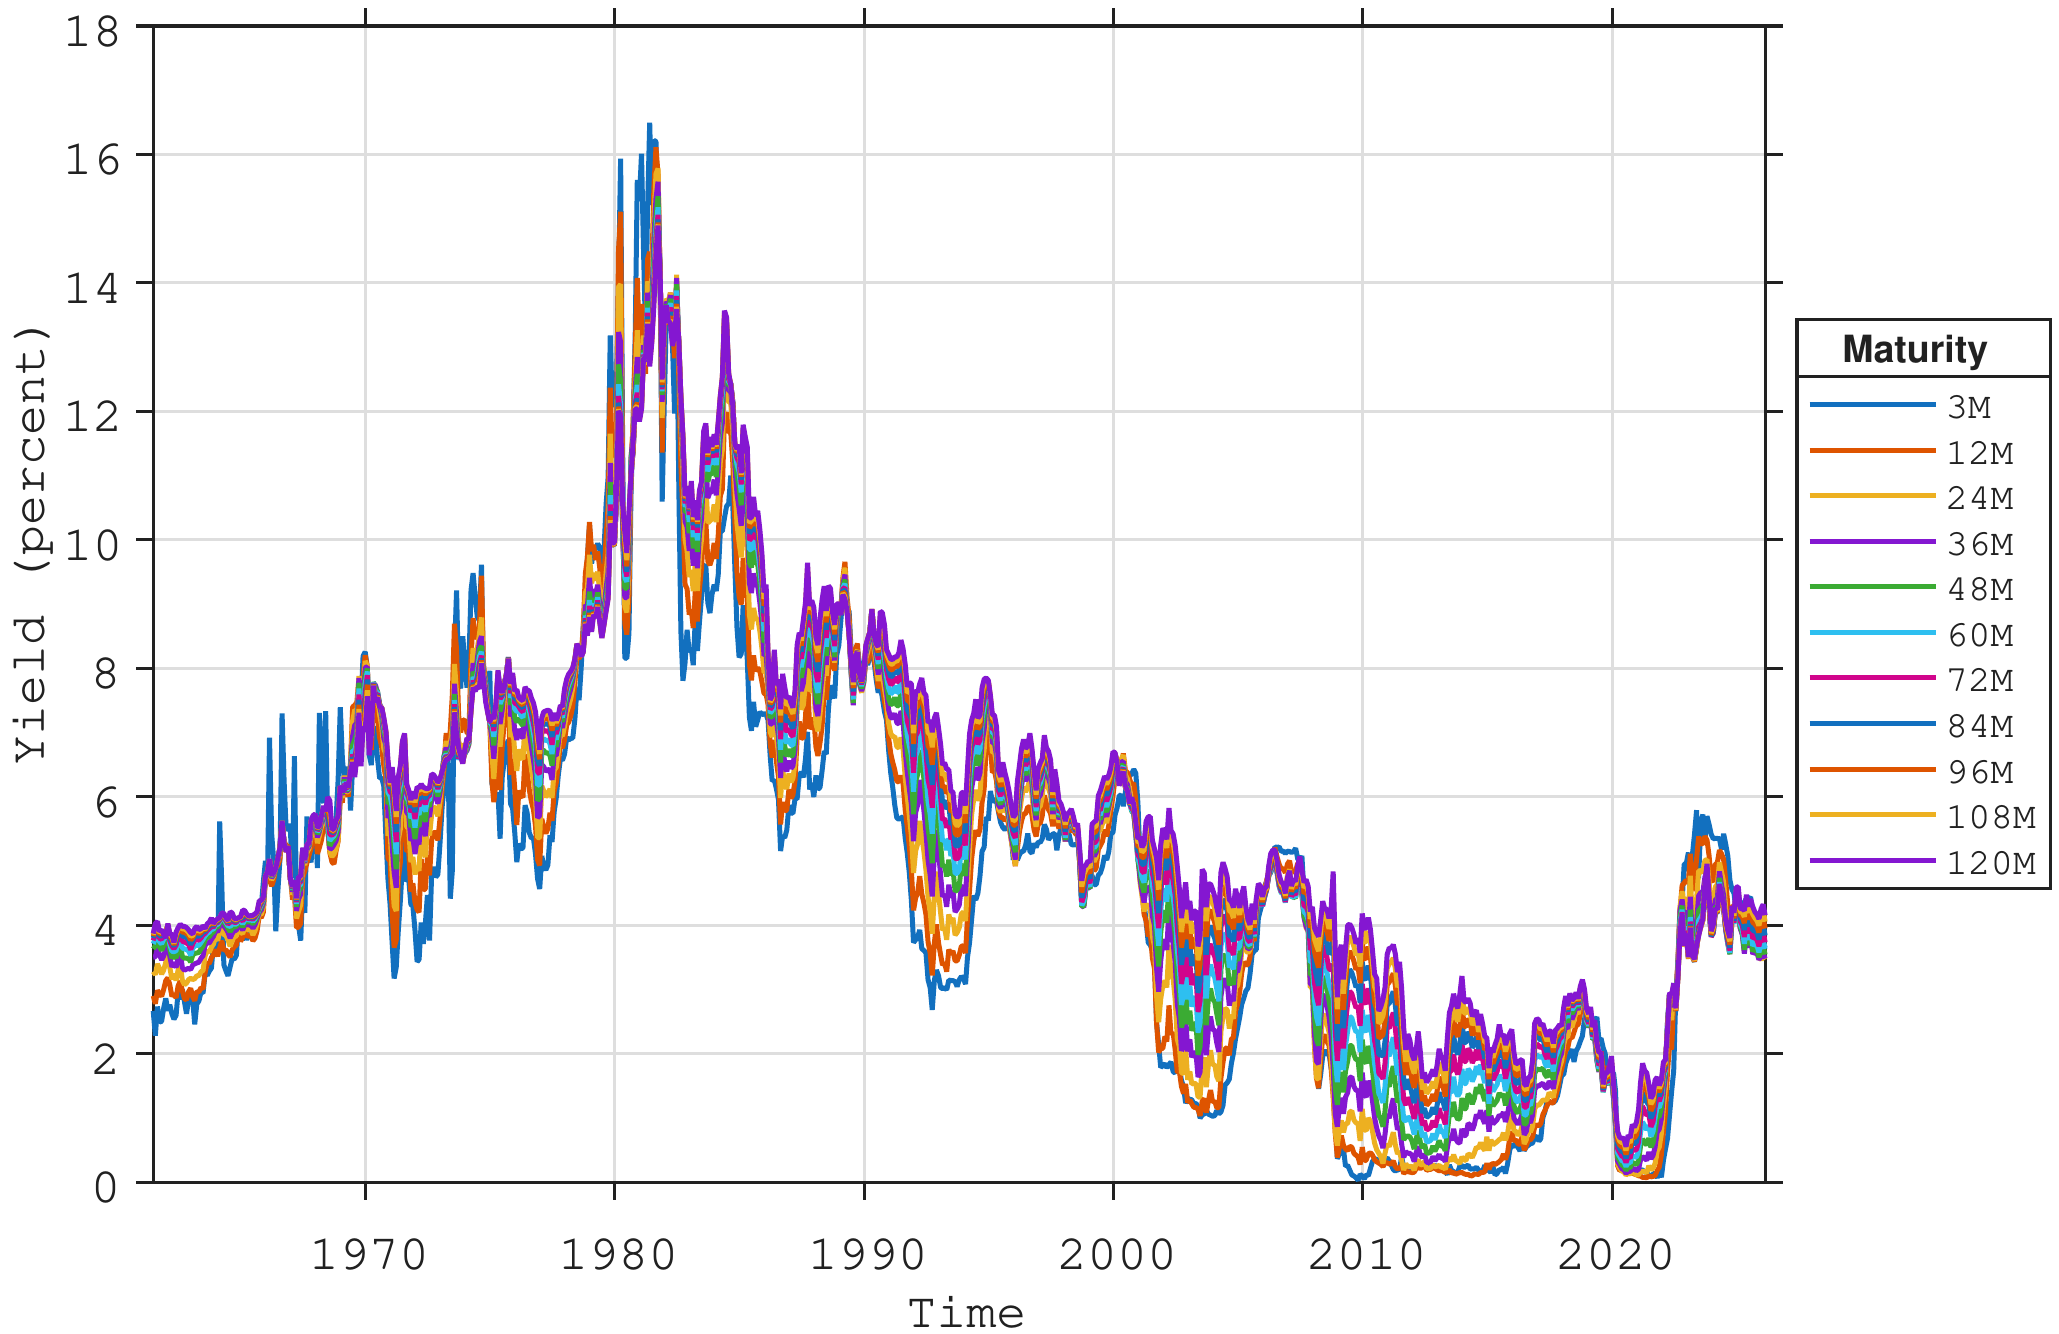
\includegraphics[width=0.85\linewidth,height=\textheight,keepaspectratio]{img/GSW_yieldcurve.png}

}

\caption{\label{fig-gsw-yieldcurve}Term structure of yields}

\end{figure}%

Estimating Equation~\ref{eq-AR1-1} for the three-month zero-coupon yield
produces the parameter estimates reported in Table~\ref{tbl-ar1-m3}. The
constant term is small and only marginally significant, while the
autoregressive coefficient is very close to unity, indicating a high
degree of persistence in the short rate. The estimated innovation
variance \(\sigma_{\varepsilon}^{2}\) reflects the conditional
volatility of unexpected changes in the rate. Together, the constant and
autoregressive coefficient imply an unconditional mean of approximately
\(4.7\%\).

\begin{longtable}[]{@{}lcc@{}}
\caption{AR(1) estimates for the 3-month
yield}\label{tbl-ar1-m3}\tabularnewline
\toprule\noalign{}
Parameter & Estimate & Standard error \\
\midrule\noalign{}
\endfirsthead
\toprule\noalign{}
Parameter & Estimate & Standard error \\
\midrule\noalign{}
\endhead
\bottomrule\noalign{}
\endlastfoot
\(c\) (constant) & 0.0723 & 0.0353 \\
\(\rho\) (AR coefficient) & 0.9848 & 0.0062 \\
\(\sigma_{\varepsilon}^{2}\) (innovation variance) & 0.3171 & -- \\
Implied unconditional mean & 4.7408 & -- \\
\end{longtable}

Inserting the parameter estimates from Table~\ref{tbl-ar1-m3} into the
expression for the short-rate derived yield curve in
Equation~\ref{eq-sr-yieldCurve} allows for estimating the model based
yield curves. Figure~\ref{fig-model-based-yieldcurve-estimates-ar1}
compares the model based yield curves obtained from the AR(1) model for
the short rate under the \(\mathbb{P}\)-measure.

\begin{figure}

\centering{

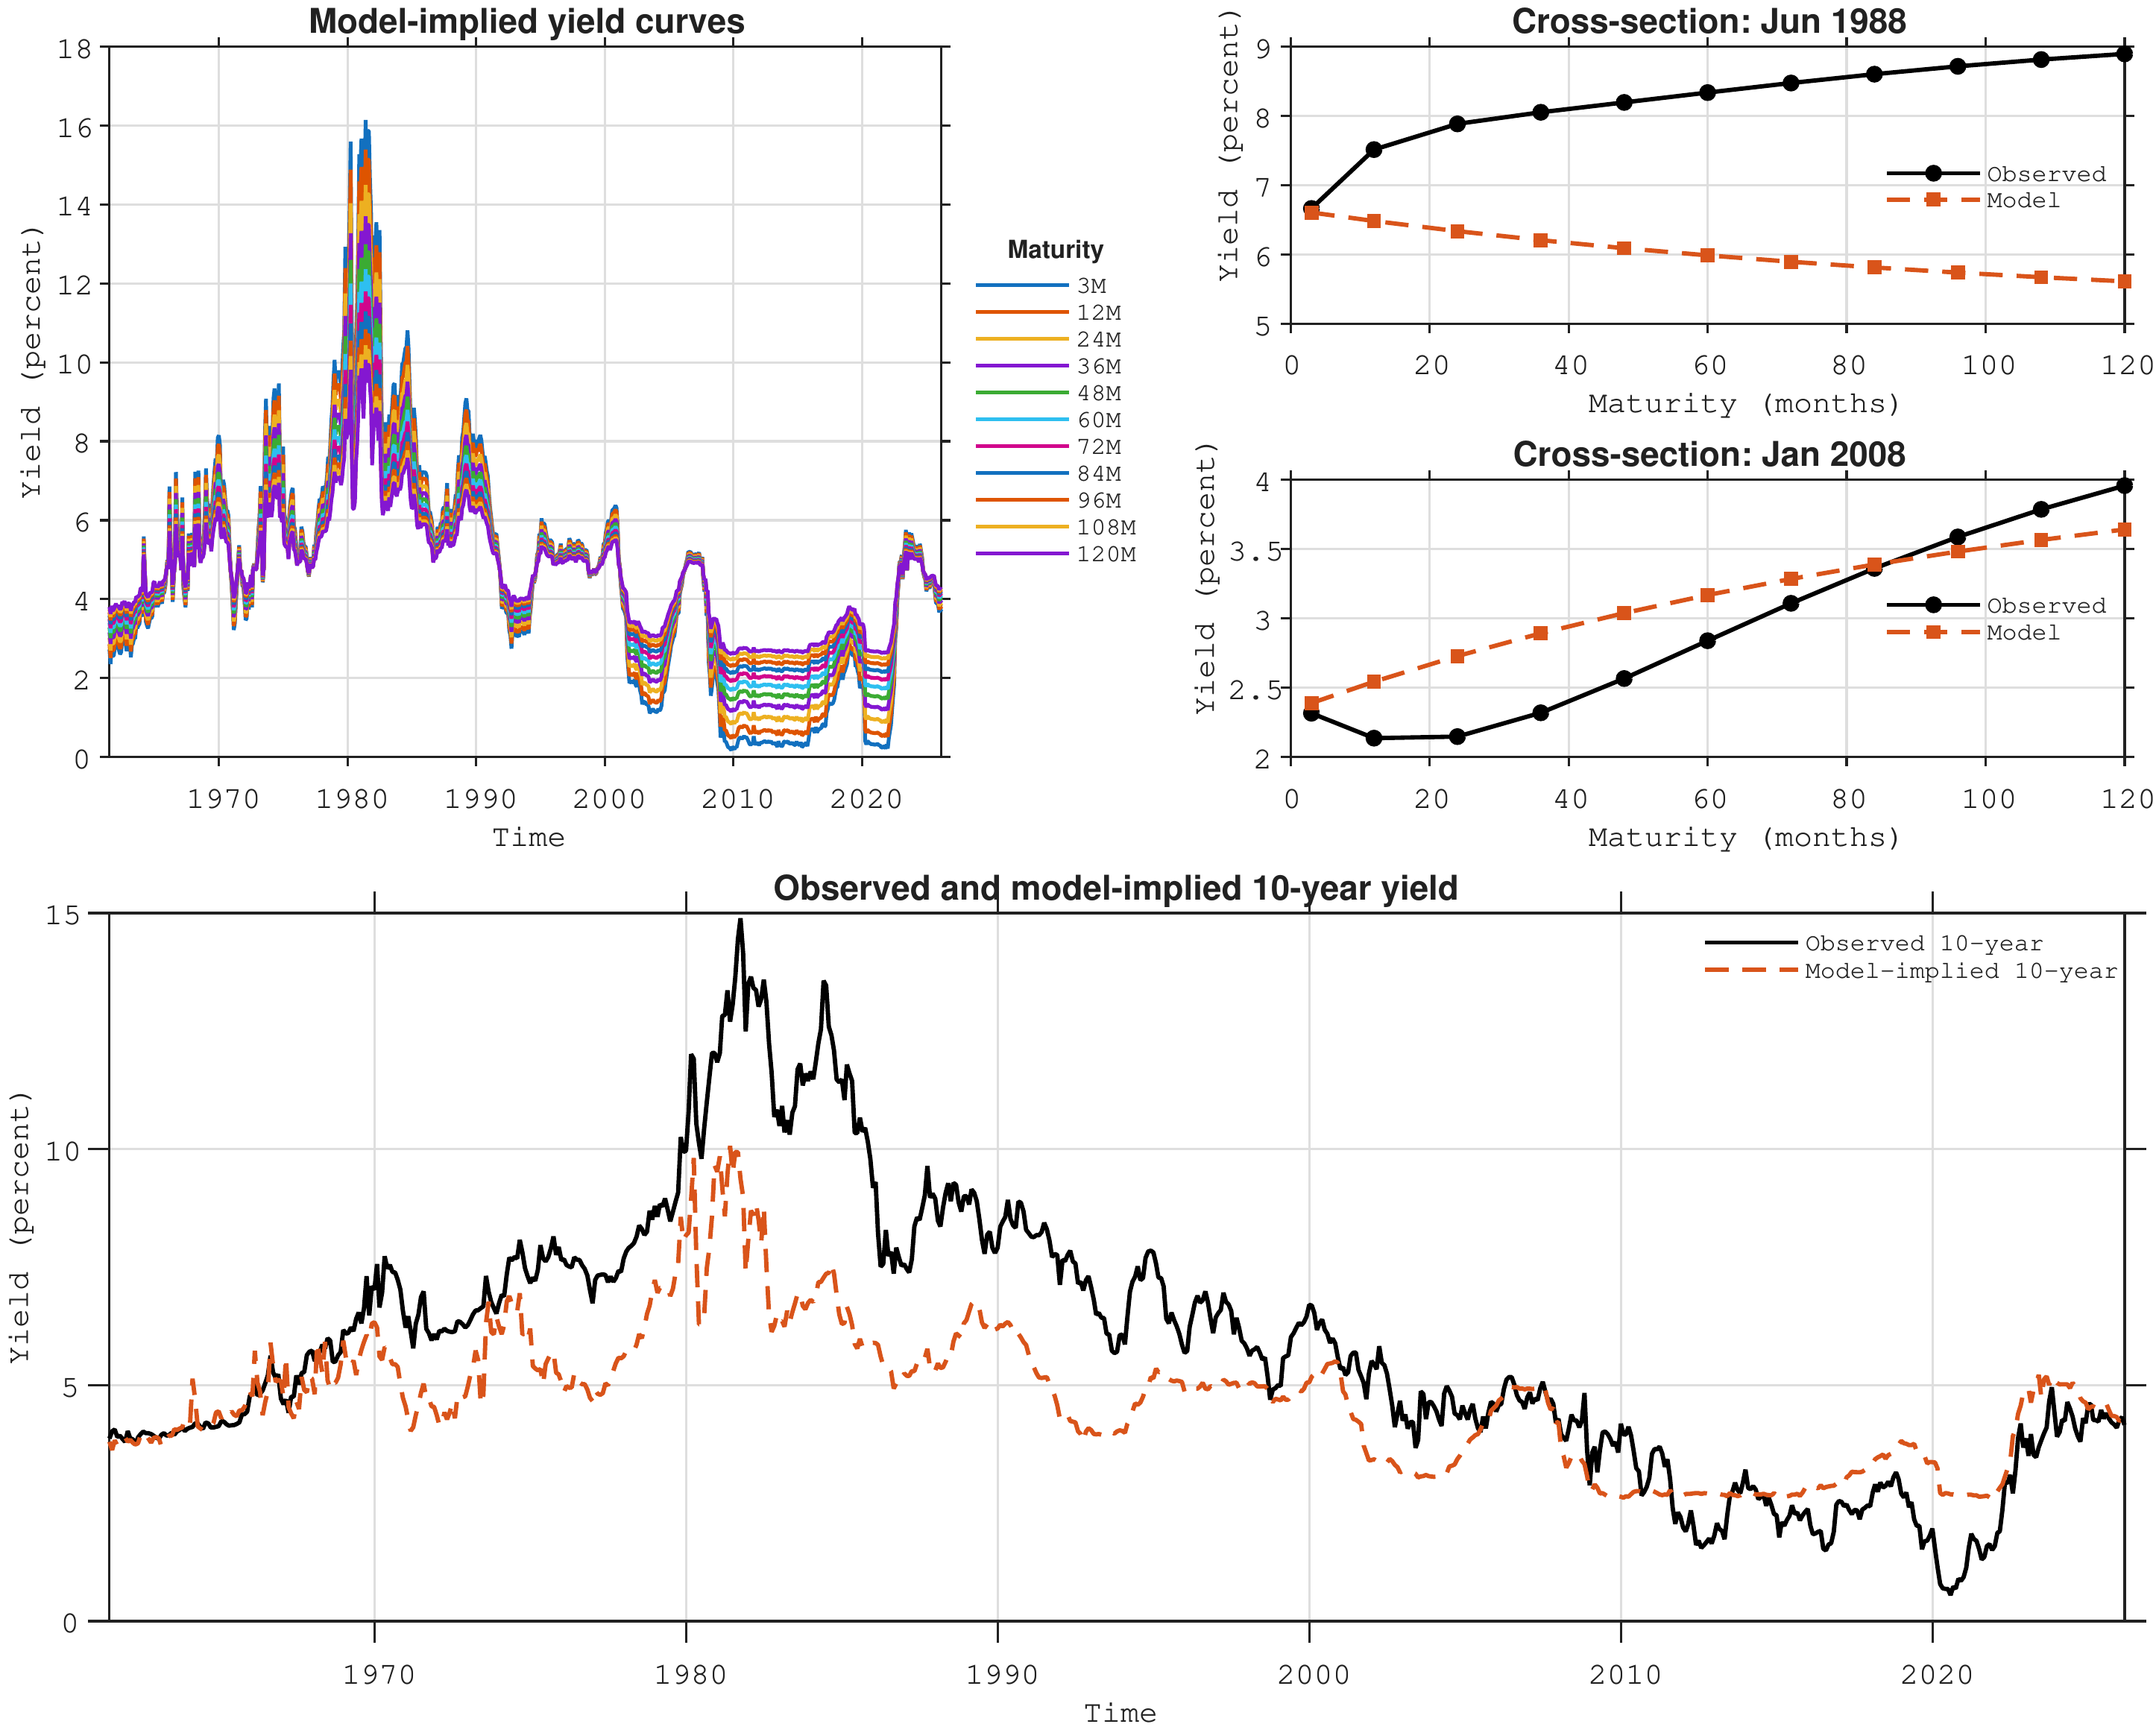
\includegraphics[width=0.85\linewidth,height=\textheight,keepaspectratio]{img/AR1_yieldcurve_P_measure.png}

}

\caption{\label{fig-model-based-yieldcurve-estimates-ar1}Yields under
the \(\mathbb{P}\)-measure}

\end{figure}%

\emph{The figure shows model‑implied zero‑coupon yields for maturities
from 3 months to 10 years under the \(\mathbb{P}\)‑measure, obtained
from an AR(1) specification for the short‑rate dynamics with parameter
estimates given in Table~Table~\ref{tbl-ar1-m3}. The top‑left panel
shows the time‑series evolution of the model‑implied yields at all
maturities contained in the original data set
(Figure~Figure~\ref{fig-gsw-yieldcurve}). The top‑right panel compares
the observed and model‑implied \(\mathbb{P}\)‑measure yield curves for
two selected dates. The bottom panel compares the observed and
model‑implied 10‑year yield over the full sample from 1960 to 2026.}

Figure~\ref{fig-model-based-yieldcurve-estimates-ar1} provides an
illustration of how the AR(1) short‑rate model translates into yield
curves at each time step covered by the data sample. As mentioned above,
this yield curve surface does not embed any correction for risk premia.
The wedge between the observed yields and the \(\mathbb{P}\)-measure
yields therefore represents the existence of risk premia - and the need
for integrating those in the model.

In the top‑left panel of the figure the model‑implied zero‑coupon yields
for maturities ranging from 3 months to 10 years are shown. Each
coloured line corresponds to a particular maturity, and all curves are
generated from an AR(1) representation of the short rate using the
parameter estimates reported in Table~\ref{tbl-ar1-m3}. Several features
stand out. First, since the model relies on a single factor (the short
rate) the model produces curves that move in parallel over time. The
level of the whole curve tracks the underlying short‑rate dynamics, with
higher short‑rate regimes in the 1970s and early 1980s associated with a
generally higher model‑implied term structure, and the low‑rate
environment after the global financial crisis leading to persistently
low model‑implied yields. Second, the dispersion across maturities is
modest: long‑term yields are only slightly above short‑term yields,
reflecting the fact that under the \(\mathbb{P}\)‑measure the curve is
essentially determined by averages of expected future short rates.

The top‑right panels compare observed and model‑implied yield curves for
two specific cross‑sections. These snapshots highlight the role of risk
premia. In the first example, taken from a high‑rate environment, the
observed yield curve is noticeably steeper than the model‑implied curve,
especially at longer maturities. While the AR(1) model implies a
relatively moderate upward slope -- consistent with expectations of
future short‑rate mean reversion -- market yields at intermediate and
long maturities lie substantially above the \(\mathbb{P}\)‑measure
curve. The wedge between the two curves is naturally interpreted as a
positive term premium: investors require extra compensation to hold
long‑dated bonds when interest‑rate uncertainty is high. In the second
cross‑section, taken from a low‑rate or stressed environment, the
pattern may reverse or flatten, with observed long‑term yields in some
cases closer to, or even below, the model‑implied values. This reflects
periods in which term premia are compressed or even negative, for
instance when there is strong demand for safe long‑dated assets or when
monetary policy guidance anchors expectations about future short rates.
These yield-curve plots make it clear that the limited flexibility of
the one‑factor model prevents it from fully reproducing the shapes of
the observed yield curves.

The bottom panel focuses on the 10‑year maturity and compares the
full‑sample evolution of the observed yield with its model‑implied
counterpart. The model‑implied 10‑year yield inherits the smoothness of
the AR(1) short‑rate process: it co‑moves with the observed yield over
the business cycle and correctly captures broad low‑ and high‑rate
regimes, but it displays smaller peaks and shallower troughs. In the
high‑inflation period of the late 1970s and early 1980s, for example,
the observed 10‑year yield rises far above the model‑implied level,
indicating a substantial positive term premium compensated investors for
heightened inflation and interest‑rate risk. Conversely, in more recent
decades the observed 10‑year yield frequently lies close to, or below,
the model‑implied curve, signalling compressed or negative term premia
consistent with accommodative monetary policy, quantitative easing and
safe‑asset scarcity.

Overall, this highlights two key messages. First, a very parsimonious
AR(1) model for the short rate (under the \(\mathbb{P}\)‑measure) is
able to reproduce the dynamic evolution of the short rate in the time
series dimension, and broad-based movements in the yield curve. Second,
and more importantly for asset‑pricing applications, systematic and
time‑varying deviations between observed and model‑implied yields
provide direct evidence of risk premia embedded in bond prices. These
risk premia are economically significant at longer maturities and vary
across regimes, underscoring the need for models that go beyond pure
expectations of future short rates when pricing and managing
fixed‑income portfolios.

\section{\texorpdfstring{Risk premia and the \(\mathbb{P}\) and
\(\mathbb{Q}\)
measures}{Risk premia and the \textbackslash mathbb\{P\} and \textbackslash mathbb\{Q\} measures}}\label{risk-premia-and-the-mathbbp-and-mathbbq-measures}

To introduce risk premia in a one‑factor setting, we follow Vasicek
(1977). He presents a simple and tractable model where the distinction
between the \(\mathbb{P}\) and \(\mathbb{Q}\) measure dynamics is
explicit, and where the role played by risk premia is clear. In other
models, as we will see later, this principle is extended to a
multi-factor setting. But, for clarity, it is probably easier to start
with a 1-factor model first. Although Vasicek formulates his model in
continuous time, we work in discrete time to maintain consistency with
the rest of the book.

Under the (historical) \(\mathbb{P}\) measure, Vasicek assumes that the
short rate follows a mean-reverting Gaussian autoregressive process of
order 1, which is the discrete-time analogue of a mean-reverting
diffusion for the short rate.
\begin{align}
    r_t &= \mu^{\mathbb{P}} + \rho^{\mathbb{P}} \, (r_{t-1} - \mu^{\mathbb{P}}) + \varepsilon^{\mathbb{P}}_t, \quad \varepsilon^{\mathbb{P}}_t \sim N(0, \sigma_{\mathbb{P}}^2),
\end{align}
This is the AR(1) process we looked at in the previous section in
Equation~\ref{eq-ar1}; but here it is made explicit that this process
evolves under the \(\mathbb{P}\) measure, which is equal to the dynamics
expressed by historical data. The requirements of stationarity also
apply here.

In addition to the \(\mathbb{P}\), also \(\mathbb{Q}\) measure dynamics
are assumed for the short rate:
\begin{align}
    r_t &= \mu^{\mathbb{Q}} + \rho^{\mathbb{Q}} \, (r_{t-1} - \mu^{\mathbb{Q}}) + \varepsilon^{\mathbb{Q}}_t, \quad \varepsilon^{\mathbb{Q}}_t \sim N(0, \sigma_{\mathbb{Q}}^2).
\end{align}
As it was the case in the previous section, where bond prices were
calculated under the \(\mathbb{P}\) in Equation~\ref{eq-P-P}, bond
prices can similarly be calculated under the \(\mathbb{Q}\) measure:
\begin{equation}\protect\phantomsection\label{eq-P-Q}{
\begin{align}
         \mathbb{E}_t^{\mathbb{Q}} \left[P_t^{(n)}\right] = \mathbb{E}^{\mathbb{Q}}_t\left[ e^{-\sum^{n}_{t=1} r_t\Delta t} \right].
\end{align}
}\end{equation}

The sum \(\sum_{j=0}^{n-1} r_{t+j}\) is the discrete-time analogue of
the integral of the short rate that appears in continuous-time models.

As we saw in Figure~\ref{fig-model-based-yieldcurve-estimates-ar1}, the
estimated \(\mathbb{P}\)-dynamics do not generate bond prices (and thus
zero-coupon yields) that fit the data particularly well. In contrast,
the \(\mathbb{Q}\)-measure is constructed precisely so that the model
can match the observed cross-section of bond prices and zero-coupon
yields as closely as possible. However, the presence of two different
measures naturally raises the question of how they are related: The
\(\mathbb{P}\)-measure dynamics describe the statistical behaviour of
the short rate (and hence yields) in the data, while the
\(\mathbb{Q}\)-measure dynamics must be consistent with the no-arbitrage
pricing of bonds. Moving from \(\mathbb{P}\) to \(\mathbb{Q}\) involves
adjusting the short-rate process to reflect investors' compensation for
bearing interest-rate risk; this adjustment amounts to the market price
of risk. In this sense, the \(\mathbb{P}\)-measure captures the
time-series evolution of yields, whereas the \(\mathbb{Q}\)-measure
governs their cross-sectional behaviour across maturities at a given
point in time (the shape and level of the yield curve). The same
underlying state process is therefore described in two ways: under
\(\mathbb{P}\) to match the historical dynamics, and under
\(\mathbb{Q}\) to match observed prices.

The \(\mathbb{Q}\)-measure is also often referred to as the risk-neutral
measure. This terminology can appear counter-intuitive, because it is
exactly the change from \(\mathbb{P}\) to \(\mathbb{Q}\) that embeds
risk premia into prices. The point, however, is that under
\(\mathbb{Q}\) the adjustment is made in such a way that all discounted
asset prices become martingales, so that their expected excess return
(above the risk-free rate) is zero and all cash flows therefore can be
discounted at the risk-free rate.\footnote{This is an example of the
  general idea of certainty-equivalent cash flows: the risk adjustment
  is moved into the pricing kernel (or, equivalently, into the
  probability measure under which prices are computed), so that the
  resulting cash flows can be discounted at the risk-free rate. More
  broadly, it reflects the fundamental principle that the riskiness of
  cash flows and the discount rate must be aligned.}

Leaving the model-rigour for later, and taking a purely empirical
perspective, we know that model-implied bond prices under the
\(\mathbb{Q}\)-measure have the same exponential-affine form as the
prices derived above under the \(\mathbb{P}\)-measure. Therefore,
following Equation~\ref{eq-sr-yieldCurve}, Equation~\ref{eq-An}, and
Equation~\ref{eq-Bn} we can write
\begin{equation}\protect\phantomsection\label{eq-sr-yieldCurve-Q}{
\begin{align}
    \mathbb{E}_t^{\mathbb{Q}}(y_t^{(n)})
    &= \frac{1}{n}\,\mathbb{E}_t^{\mathbb{Q}}\!\left(A_n + B_n r_t\right)
        \nonumber \\
    &= \mathbb{E}_t^{\mathbb{Q}}\!\left(a_n + b_n r_t\right),
\end{align}
}\end{equation}

which implies that
\begin{equation}\protect\phantomsection\label{eq-An-Bn-Q}{
\begin{align}
    A_n^{\mathbb{Q}}
    &= \frac{c^{\mathbb{Q}}\,n}{1-\rho^{\mathbb{Q}}}
        - \frac{c^{\mathbb{Q}}\big(\rho^{\mathbb{Q}}
        - \left(\rho^{\mathbb{Q}}\right)^{(n+1)}\big)}
               {\big(1-\rho^{\mathbb{Q}}\big)^2}, 
        \qquad \text{and} \\
    B_n^{\mathbb{Q}}
    &= \frac{\rho^{\mathbb{Q}}-\left(\rho^{\mathbb{Q}}\right)^{(n+1)}}
             {1-\rho^{\mathbb{Q}}}.
\end{align}
}\end{equation} Similarly, under the historical measure we have
\begin{equation}\protect\phantomsection\label{eq-sr-yieldCurve-P}{
\begin{align}
    \mathbb{E}_t^{\mathbb{P}}(y_t^{(n)})
    &= \frac{1}{n}\,\mathbb{E}_t^{\mathbb{P}}\!\left(A_n + B_n \, r_t\right)
        \nonumber \\
    &= \mathbb{E}_t^{\mathbb{P}}\!\left(a_n + b_n\, r_t\right),
\end{align}
}\end{equation} implying
\begin{equation}\protect\phantomsection\label{eq-An-Bn-P}{
\begin{align}
    A_n^{\mathbb{P}}
    &= \frac{c^{\mathbb{P}}\,n}{1-\rho^{\mathbb{P}}}
        - \frac{c^{\mathbb{P}}\big(\rho^{\mathbb{P}}
        - \left(\rho^{\mathbb{P}}\right)^{(n+1)}\big)}
               {\big(1-\rho^{\mathbb{P}}\big)^2}, 
        \qquad \text{and} \\
    B_n^{\mathbb{P}}
    &= \frac{\rho^{\mathbb{P}}-\left(\rho^{\mathbb{P}}\right)^{(n+1)}}
             {1-\rho^{\mathbb{P}}}.
\end{align}
}\end{equation}

The model-implied term premia are then given by the difference between
the \(\mathbb{Q}\) and \(\mathbb{P}\) expected yields,
\begin{equation}\protect\phantomsection\label{eq-TP-def}{
\begin{align}
    \theta_t^{(n)} = \mathbb{E}_t^{\mathbb{Q}}(y_t^{(n)}) - \mathbb{E}_t^{\mathbb{P}}(y_t^{(n)})
    &= \big(a_n^{\mathbb{Q}} - a_n^{\mathbb{P}}\big)
        + \big(b_n^{\mathbb{Q}} - b_n^{\mathbb{P}}\big)\, r_t,
\end{align}
}\end{equation}

with \(a_n^{\mathbb{Q}} = A_n^{\mathbb{Q}}/n\) and
\(a_n^{\mathbb{P}} = A_n^{\mathbb{P}}/n\), and similarly
\(b_n^{\mathbb{Q}} = B_n^{\mathbb{Q}}/n\) and
\(b_n^{\mathbb{P}} = B_n^{\mathbb{P}}/n\).

To ensure consistent market pricing and adherence to the no‑arbitrage
principle, recall that bond prices are obtained from a single stochastic
discount factor (SDF) \(\mathcal{M}\), as in
Equation~\ref{eq-fundamentalPrice} and repeated here:
\begin{align}
    P_t^{(n)} &= \mathbb{E}_t\!\left( \mathcal{M}_{t+1} \, P_{t+1}^{\,n-1} \right). \nonumber
\end{align}
A functional form has to be chosen for \(\mathcal{M}\), and in Gaussian
term‑structure models it is standard to work with a log‑normal
one‑period pricing kernel of the form
\begin{align}
   M_{t+1} &= \exp\left( -r_t - \frac{1}{2}\lambda_t^{2} - \lambda_t e_{t+1}^{\mathbb{P}} \right),
\end{align}
where \(e_{t+1}^{\mathbb{P}}\) is the \(\mathbb{P}\)‑innovation in the
short‑rate process and \(\lambda_t\) is the (possibly state‑dependent)
market price of risk. In this specification the log SDF is affine in the
short rate shock \(e_{t+1}\), so \(\mathcal{M}_{t+1}\) itself is
log‑normally distributed.

Intuitively, the first term, \(-r_t\), accounts for the time-value of
money, and the two terms involving \(\lambda_t\) incorporate the
compensation for bearing risk: The term \(-\tfrac{1}{2}\lambda_t^2\)
depends only on the magnitude of the market price of risk and is always
negative; it lowers the average value of \(M_{t+1}\) and thus lowers
bond prices.\footnote{Formally, this term ensures that, after the change
  of measure to \(\mathbb{Q}\), discounted asset prices are martingales.}
The term \(-\lambda_t e_{t+1}^{\mathbb{P}}\) links the SDF directly to
the short‑rate shock: when \(e_{t+1}^{\mathbb{P}}\) is positive (a
positive short‑rate innovation, which is typically bad for bond values),
the exponent becomes more negative and \(M_{t+1}\) is smaller, so
pay‑offs in those states are discounted more heavily. When
\(e_{t+1}^{\mathbb{P}}\) is negative (a negative short‑rate innovation,
which is favourable for bond values), the exponent is larger and
\(M_{t+1}\) increases, so pay‑offs in those states receive more weight.
In this way, \(\lambda_t\) governs how much extra value investors assign
to pay‑offs that arrive in ``bad'' interest‑rate states, and the
resulting state‑dependent reweighting generates coherent risk premia
across all maturities and assets priced by the same SDF.

The next step is to parameterise \(\lambda_t\), the market price of
risk. In the term‑structure literature it is standard to assume that
\(\lambda_t\) is an affine function of the state variables. In the
one‑factor short-rate setting, this reduces to a simple linear
dependence on the short rate:
\begin{equation}\protect\phantomsection\label{eq-marketPriceOfRisk}{
\begin{align}
    \lambda_t &= \lambda_0 + \lambda_1 \, r_t,
\end{align}
}\end{equation} where \(\lambda_0\) and \(\lambda_1\) are constants. The
intercept \(\lambda_0\) captures a level component of risk compensation
that is independent of the current interest‑rate level, while the slope
coefficient \(\lambda_1\) allows the market price of short‑rate risk to
vary systematically with \(r_t\).

As shown above and exemplified by Equation~\ref{eq-TP-def}, the
\(\mathbb{P}\) and \(\mathbb{Q}\) measure parameters are connected
through risk adjustment performed by the market price of risk in
Equation~\ref{eq-marketPriceOfRisk}. Inspecting short-rate process under
the historical measure \(\mathbb{P}\):
\begin{equation}\protect\phantomsection\label{eq-vasicek-P-drift}{
\begin{align}
    r_t &= \alpha^{\mathbb{P}} + \rho^{\mathbb{P}} \, r_{t-1} 
            + \varepsilon_t^{\mathbb{P}}, \qquad
            \varepsilon_t^{\mathbb{P}} \sim N(0,\sigma^2),
\end{align}
}\end{equation} it is seen that all randomness enters through the
one-period innovation \(\varepsilon_t^{\mathbb{P}}\). Economically, this
innovation represents the unexpected component of monetary policy and
macro-financial news at each date; conditional on \(r_{t-1}\),
everything else in Equation~\ref{eq-vasicek-P-drift} is deterministic.
When switching to the pricing measure, \(\mathbb{Q}\), the SDF injects
equilibrium investor preferences (risk premia) by adjusting the economic
importance on these shocks (i.e.~it reweights the shocks) to obtain
market prices that reflect the market's assessment of the price of risk.

It is common to assume that this risk adjustment effects the
distribution of the innovation under the pricing measure \(\mathbb{Q}\)
by shifting the mean of the shock but leaving the variance unchanged. We
can therefore define the \(\mathbb{Q}\)-innovation as a shifted version
of the \(\mathbb{P}\)-innovation in the following way:
\begin{equation}\protect\phantomsection\label{eq-eps-Q-def2}{
\begin{align}
    \varepsilon_{t+1}^{\mathbb{Q}}
    &= \varepsilon_{t+1}^{\mathbb{P}} + \sigma \lambda_t.
\end{align}
}\end{equation} Effectively, the short-rate shock under \(\mathbb{Q}\)
has the same variance \(\sigma^2\) as under \(\mathbb{P}\), but its mean
is shifted by \(\sigma \lambda_t\). The scaling by \(\sigma\) reflects
that \(\lambda_t\) is expressed as a price-per-unit-of-risk metric: a
given value of \(\lambda_t\) corresponds to a larger level drift
correction when the innovation is more volatile. The total drift
adjustment is therefore of the form:
volatility-times-price-of-risk.\footnote{Formally, the change of measure
  from \(\mathbb{P}\) to \(\mathbb{Q}\) is implemented via the
  Radon--Nikodym derivative, which expresses how probabilities under
  \(\mathbb{Q}\) are obtained by reweighting probabilities under
  \(\mathbb{P}\). In the Gaussian, log-normal SDF case considered, this
  Radon--Nikodym derivative is exponential in \(e_{t+1}^{\mathbb{P}}\),
  and the standard result of exponential tilting of normal distributions
  implies exactly the mean shift in Equation~\ref{eq-eps-Q-def2}.}

Substituting Equation~\ref{eq-eps-Q-def2} into the
\(\mathbb{P}\)-dynamics Equation~\ref{eq-vasicek-P-drift} gives
\begin{equation}\protect\phantomsection\label{eq-rt-sub-epsQ}{
\begin{align}
    r_t 
    &= \alpha^{\mathbb{P}} + \rho^{\mathbb{P}} r_{t-1} + \varepsilon_t^{\mathbb{P}} \nonumber \\
    &= \alpha^{\mathbb{P}} + \rho^{\mathbb{P}} r_{t-1} 
        + \big( \varepsilon_t^{\mathbb{Q}} - \sigma \lambda_{t-1} \big),
\end{align}
}\end{equation} Inserting Equation~\ref{eq-marketPriceOfRisk} into
Equation~\ref{eq-rt-sub-epsQ} and collecting terms yields
\begin{equation}\protect\phantomsection\label{eq-rt-Q-ar1}{
\begin{align}
    r_t
    &= \alpha^{\mathbb{P}} + \rho^{\mathbb{P}} r_{t-1} 
        + \varepsilon_t^{\mathbb{Q}} - \sigma (\lambda_0 + \lambda_1 r_{t-1}) \nonumber \\
    &= \big(\alpha^{\mathbb{P}} - \sigma \lambda_0\big) 
        + \big(\rho^{\mathbb{P}} - \sigma \lambda_1\big) r_{t-1}
        + \varepsilon_t^{\mathbb{Q}}.
\end{align}
}\end{equation} Under the pricing measure \(\mathbb{Q}\), the short rate
still follows an AR(1) process, with the same innovation variance as
under \(\mathbb{P}\), but with risk-adjusted intercept and persistence
parameters:
\begin{equation}\protect\phantomsection\label{eq-alphaQ-def}{
\begin{align}
    \alpha^{\mathbb{Q}} &= \alpha^{\mathbb{P}} - \sigma \lambda_0, 
\end{align}
}\end{equation}

\begin{equation}\protect\phantomsection\label{eq-rhoQ-def}{
\begin{align}
    \rho^{\mathbb{Q}}   &= \rho^{\mathbb{P}} - \sigma \lambda_1,
\end{align}
}\end{equation} which gives:
\begin{equation}\protect\phantomsection\label{eq-vasicek-Q-drift-ar1}{
\begin{align}
    r_t &= \alpha^{\mathbb{Q}} + \rho^{\mathbb{Q}} r_{t-1} + \varepsilon_t^{\mathbb{Q}}.
\end{align}
}\end{equation}

Writing the historical and pricing-measure dynamics in mean-reverting
form is then given by:
\begin{equation}\protect\phantomsection\label{eq-vasicek-P-meanrev}{
\begin{align}
    r_t 
    &= \mu^{\mathbb{P}} + \rho^{\mathbb{P}} (r_{t-1} - \mu^{\mathbb{P}}) 
        + \varepsilon_t^{\mathbb{P}}, 
        \qquad \varepsilon_t^{\mathbb{P}} \sim N(0,\sigma^2), 
\end{align}
}\end{equation}

\begin{equation}\protect\phantomsection\label{eq-vasicek-Q-meanrev}{
\begin{align}
    r_t 
    &= \mu^{\mathbb{Q}} + \rho^{\mathbb{Q}} (r_{t-1} - \mu^{\mathbb{Q}}) 
        + \varepsilon_t^{\mathbb{Q}}, 
        \qquad \varepsilon_t^{\mathbb{Q}} \sim N(0,\sigma^2).
\end{align}
}\end{equation} with
\begin{equation}\protect\phantomsection\label{eq-muP-def}{
\begin{align}
    \mu^{\mathbb{P}} 
    = \frac{\alpha^{\mathbb{P}}}{1-\rho^{\mathbb{P}}}
    \quad \texttt{and} \quad   \mu^{\mathbb{Q}} 
    = \frac{\alpha^{\mathbb{Q}}}{1-\rho^{\mathbb{Q}}}.
\end{align}
}\end{equation} Consequently, once the historical dynamics
\((\mu^{\mathbb{P}},\rho^{\mathbb{P}})\) and the affine market price of
risk \((\lambda_0,\lambda_1)\) are specified, the no-arbitrage SDF pins
down the corresponding risk-neutral dynamics
\((\mu^{\mathbb{Q}},\rho^{\mathbb{Q}})\); they can no longer be treated
as free parameters. The wedge between the \(\mathbb{P}\)- and
\(\mathbb{Q}\)-parameters, and hence between
\(\mathbb{E}_t^{\mathbb{P}}(y_t^{(n)})\) and
\(\mathbb{E}_t^{\mathbb{Q}}(y_t^{(n)})\), is entirely driven by the
market price of risk and the volatility of the short-rate shocks. In
this way the Vasicek model provides a simple one-factor illustration of
how an explicit SDF simultaneously determines the historical and
risk-neutral dynamics and generates affine term premia.

\bookmarksetup{startatroot}

\chapter{Multi factor models}\label{multi-factor-models}

A dynamic yield curve model driven by a single factor provides a natural
starting point for thinking about interest rate risk. Yields at all
maturities move together, so that the entire term structure shifts in
parallel over time. This captures the dominant level‑type variation in
the data and links directly to familiar fixed income concepts such as
modified duration, which measures the sensitivity of a bond's price to
small, parallel changes in yields. As we will see in the PCA analysis
below, this first dimension alone explains the vast majority of yield
curve variability.

However, yield changes are rarely perfectly parallel, so models that
allow for variations in slope and curvature are essential for asset
allocation, yield‑curve scenario design, and related applications. Slope
movements arise when expectations about short‑ and long‑term interest
rates diverge. For example, during a period of monetary policy easing
(when the policy rate is lowered), while long‑run inflation expectations
and expected real growth remain broadly unchanged, the curve typically
steepens as short‑term yields fall relative to long‑term yields. During
a tightening cycle, higher policy rates tend to compress the short--long
spread and thus generates a flatter curve. In practice, slope changes
can be driven from the short end (through policy actions), from the long
end (through shifts in inflation and growth expectations), or from both
segments simultaneously.

Curvature movements describe how intermediate maturities behave relative
to the short and long ends of the curve, affecting its concavity or
convexity and giving rise to hump‑shaped or inverted shapes. These
patterns are closely tied to expectations about the future path of the
policy rate. When markets anticipate that the policy rate will fall, or
remain low for an extended period, yields at the medium horizons can
move down disproportionately, and the curve then exhibits pronounced
concavity. On the other hand, expectations of a rapid and sustained
tightening often push up medium‑term yields more strongly, producing a
more convex curve with elevated rates in the central part of the
maturity spectrum.

These considerations naturally point towards modelling the term
structure within a multi‑factor framework. Principal component analysis
(PCA) provides a convenient empirical starting point for this extension.
Applied to a panel of yields across maturities, PCA extracts orthogonal
components that capture the main directions of the variation in the
data. In typical applications the first four principal components can be
interpreted as level, slope, curvature at low maturities, and curvature
at higher maturities. The first component preserves the interpretation
of the one‑factor models and represents the dominant yield curve level
movement, while the second, third and fourth components account for
changes in slope and curvature.

The empirical factor structure suggested by PCA has directly influenced
modern term‑structure modelling. Affine term‑structure models introduce
several latent factors, often with dynamics designed to match the level,
slope and curvature pattern, while maintaining consistency with
no‑arbitrage restrictions. Nelson--Siegel type models and their dynamic
extensions build these three factors into the parametric form of the
yield curve itself, providing an economically intuitive and tractable
representation. In both cases, the one‑factor perspective remains
valuable as the primary driver of yield levels, but it is complemented
by additional factors that capture the richer cross‑sectional and
time‑series behaviour observed in the data. Modelling yields within such
a multi‑factor framework therefore preserves the simplicity and
intuition of the single level factor, while offering a much more
realistic description of interest rate risk for practical applications.

\section{Empirically determining the number of yield curve
factors}\label{empirically-determining-the-number-of-yield-curve-factors}

We begin by applying principal component analysis (PCA) to the panel of
monthly US Treasury yields spanning the period from 1960 to 2026 and
covering maturities from 3 to 120 months. The data are arranged in a
\(T\times k\) matrix \(Y\), where each row contains the cross--section
of \(k=11\) yields observed at a given month, and each column
corresponds to one maturity. Before extracting factors the column
specific mean is deducted such that the sample covariance matrix of the
yields is\footnote{Note that this is done automatically the MATLAB's pca
  function.}
\begin{align}
    S = \frac{1}{T-1} Y^{\top}\, Y.
\end{align}
Since \(S\) is symmetric and positive semi--definite, it admits an
eigenvalue decomposition
\begin{align}
    S \;=\; L D L^{\top},
\end{align}
where \(L\) is the \(k\times k\) orthonormal matrix whose columns are
the eigenvectors of \(S\), and \(D\) is the diagonal matrix collecting
the corresponding eigenvalues.\footnote{See also Chapter~0.}

Ordering the eigenvalues in descending order ensures that the first few
eigenvectors capture the maximal amount of cross--sectional variance in
the yields. Projecting \(Y\) onto the eigenvectors gives the time series
of principal components. Let \(F\) be the \(T\times k\) matrix of
factors, then:
\begin{equation}\protect\phantomsection\label{eq-PCA-projection}{
\begin{align}
    Y = F\, L^{\top},
\end{align}
}\end{equation} where each column of \(F\) is the time series of one
principal component. Because \(L\) is orthonormal, such that
\((L^{\top}L\big)^{-1}=I\), this representation can be viewed as a
multivariate regression of \(Y\) on the loadings \(L\), in which the
least--squares estimator of \(F\) is particularly simple:
\begin{equation}\protect\phantomsection\label{eq-PCA-Fhat}{
\begin{align}
    \widehat{F} = Y\, L \big(L^{\top}L\big)^{-1} \;=\; Y L.
\end{align}
}\end{equation} Substituting this expression back into the
reconstruction equation shows that PCA delivers an exact factorisation
of the de--meaned data,
\begin{equation}\protect\phantomsection\label{eq-PCA-exact-recon}{
\begin{align}
    Y \;=\; \widehat{F} L^{\top}.
\end{align}
}\end{equation} In other words, the observed yield curve at each point
in time can be written as a linear combination of \(k\) orthogonal
factors, with time--varying coefficients collected in \(\widehat{F}\)
and fixed cross--sectional loadings given by the columns of \(L\).

The empirical importance of each principal component is summarised in
Table~\ref{tbl-PCA-eigenvalues}. For component \(j\) the associated
eigenvalue \(d_j\) equals the variance of that component, and the
fraction of total variance explained is
\begin{align}
    \text{Explained}_j \;=\; \frac{d_j}{\sum_{\ell=1}^k d_\ell}\times 100 .
\end{align}
The last column of the table reports the cumulative percentage explained
when successively adding more components.

\begin{longtable}[]{@{}rccc@{}}
\caption{PCA eigenvalues and explained variance for monthly US Treasury
yields.}\label{tbl-PCA-eigenvalues}\tabularnewline
\toprule\noalign{}
PC & Eigenvalue & Explained (\%) & Cumulative (\%) \\
\midrule\noalign{}
\endfirsthead
\toprule\noalign{}
PC & Eigenvalue & Explained (\%) & Cumulative (\%) \\
\midrule\noalign{}
\endhead
\bottomrule\noalign{}
\endlastfoot
1 & 99.485 & 97.667 & 97.667 \\
2 & 2.1538 & 2.114 & 99.781 \\
3 & 0.18937 & 0.186 & 99.967 \\
4 & 0.030505 & 0.030 & 99.997 \\
5 & 0.002513 & 0.002 & 100.000 \\
6 & 0.000178 & 0.000 & 100.000 \\
7 & 0.000009 & 0.000 & 100.000 \\
8 & 0.000000 & 0.000 & 100.000 \\
9 & 0.000000 & 0.000 & 100.000 \\
10 & 0.000000 & 0.000 & 100.000 \\
11 & 0.000000 & 0.000 & 100.000 \\
\end{longtable}

Table~\ref{tbl-PCA-eigenvalues} shows that the first principal component
alone explains about \(97.7\%\) of the cross--sectional variance in
monthly yields, while the second component adds roughly \(2.1\%\),
taking the cumulative share to \(99.8\%\). The third component
contributes only an additional \(0.2\%\), and from the fourth component
onwards the marginal contribution of each factor is economically
negligible. This pattern is very typical for yield curve data and
strongly suggests that a three--factor representation is more than
sufficient to capture the salient movements in the term structure data
we work with here. Of course, this results depends on the data used.

\subsection{Cross--sectional factor
loadings}\label{crosssectional-factor-loadings}

Let \(y_t\) denote the \(k\times 1\) vector of (de--meaned) yields at
time \(t\), stacked across maturities, and collect the PCA loadings in
the \(k\times k\) matrix:
\begin{align}
\Lambda = \big[\,\ell_1 \ \ell_2 \ \cdots \ \ell_k\,\big],
\end{align}
where the \(j\)th column \(\ell_j\) is the loading vector associated
with principal component \(j\). Likewise, let
\begin{align}
    f_t \;=\;
    \begin{bmatrix}
        f_{t,1} \\
        \vdots   \\
        f_{t,k}
    \end{bmatrix}
\end{align}
be the \(k\times 1\) vector of factor observations (scores) at time
\(t\). The fitted yield vector at time \(t\) can then be written
compactly as:
\begin{align}
y_t &= \Lambda f_t.
\end{align}
This shows that each cross--section of yields is obtained as a linear
combination of the principal components with time--varying coefficients
collected in \(f_t\) and fixed cross--sectional loadings given by the
columns of \(\Lambda\).

Figure~\ref{fig-PCA-loadings} plots the loadings of the first three
principal components across maturities from 3 to 120 months. Loadings
for the first component are virtually constant across the maturity
spectrum implying that this component shifts the entire yield curve up
and down by the same amount, and therefore has a naturally interpreted
as a level factor. The second panel shows that the loading of the second
component declines monotonically with maturity, implying that this
factor raises short--term yields while lowering long--term yields (or
vice versa); this principal component therefore captures changes in the
slope of the yield curve between short and long maturities. The third
loading shows a hump--shaped pattern that is aligns which the
characteristic of a curvature factor that steepens or flattens the curve
around its medium--term segment.

Together, these three components form the familiar
level--slope--curvature trio that underlies most modern dynamic yield
curve models. The fact that they emerge here purely from an unsupervised
statistical decomposition, without imposing any economic structure,
provides strong evidence that the main drivers of yield curve dynamics
are indeed low--dimensional and have a clear geometric interpretation.

\begin{figure}

\centering{

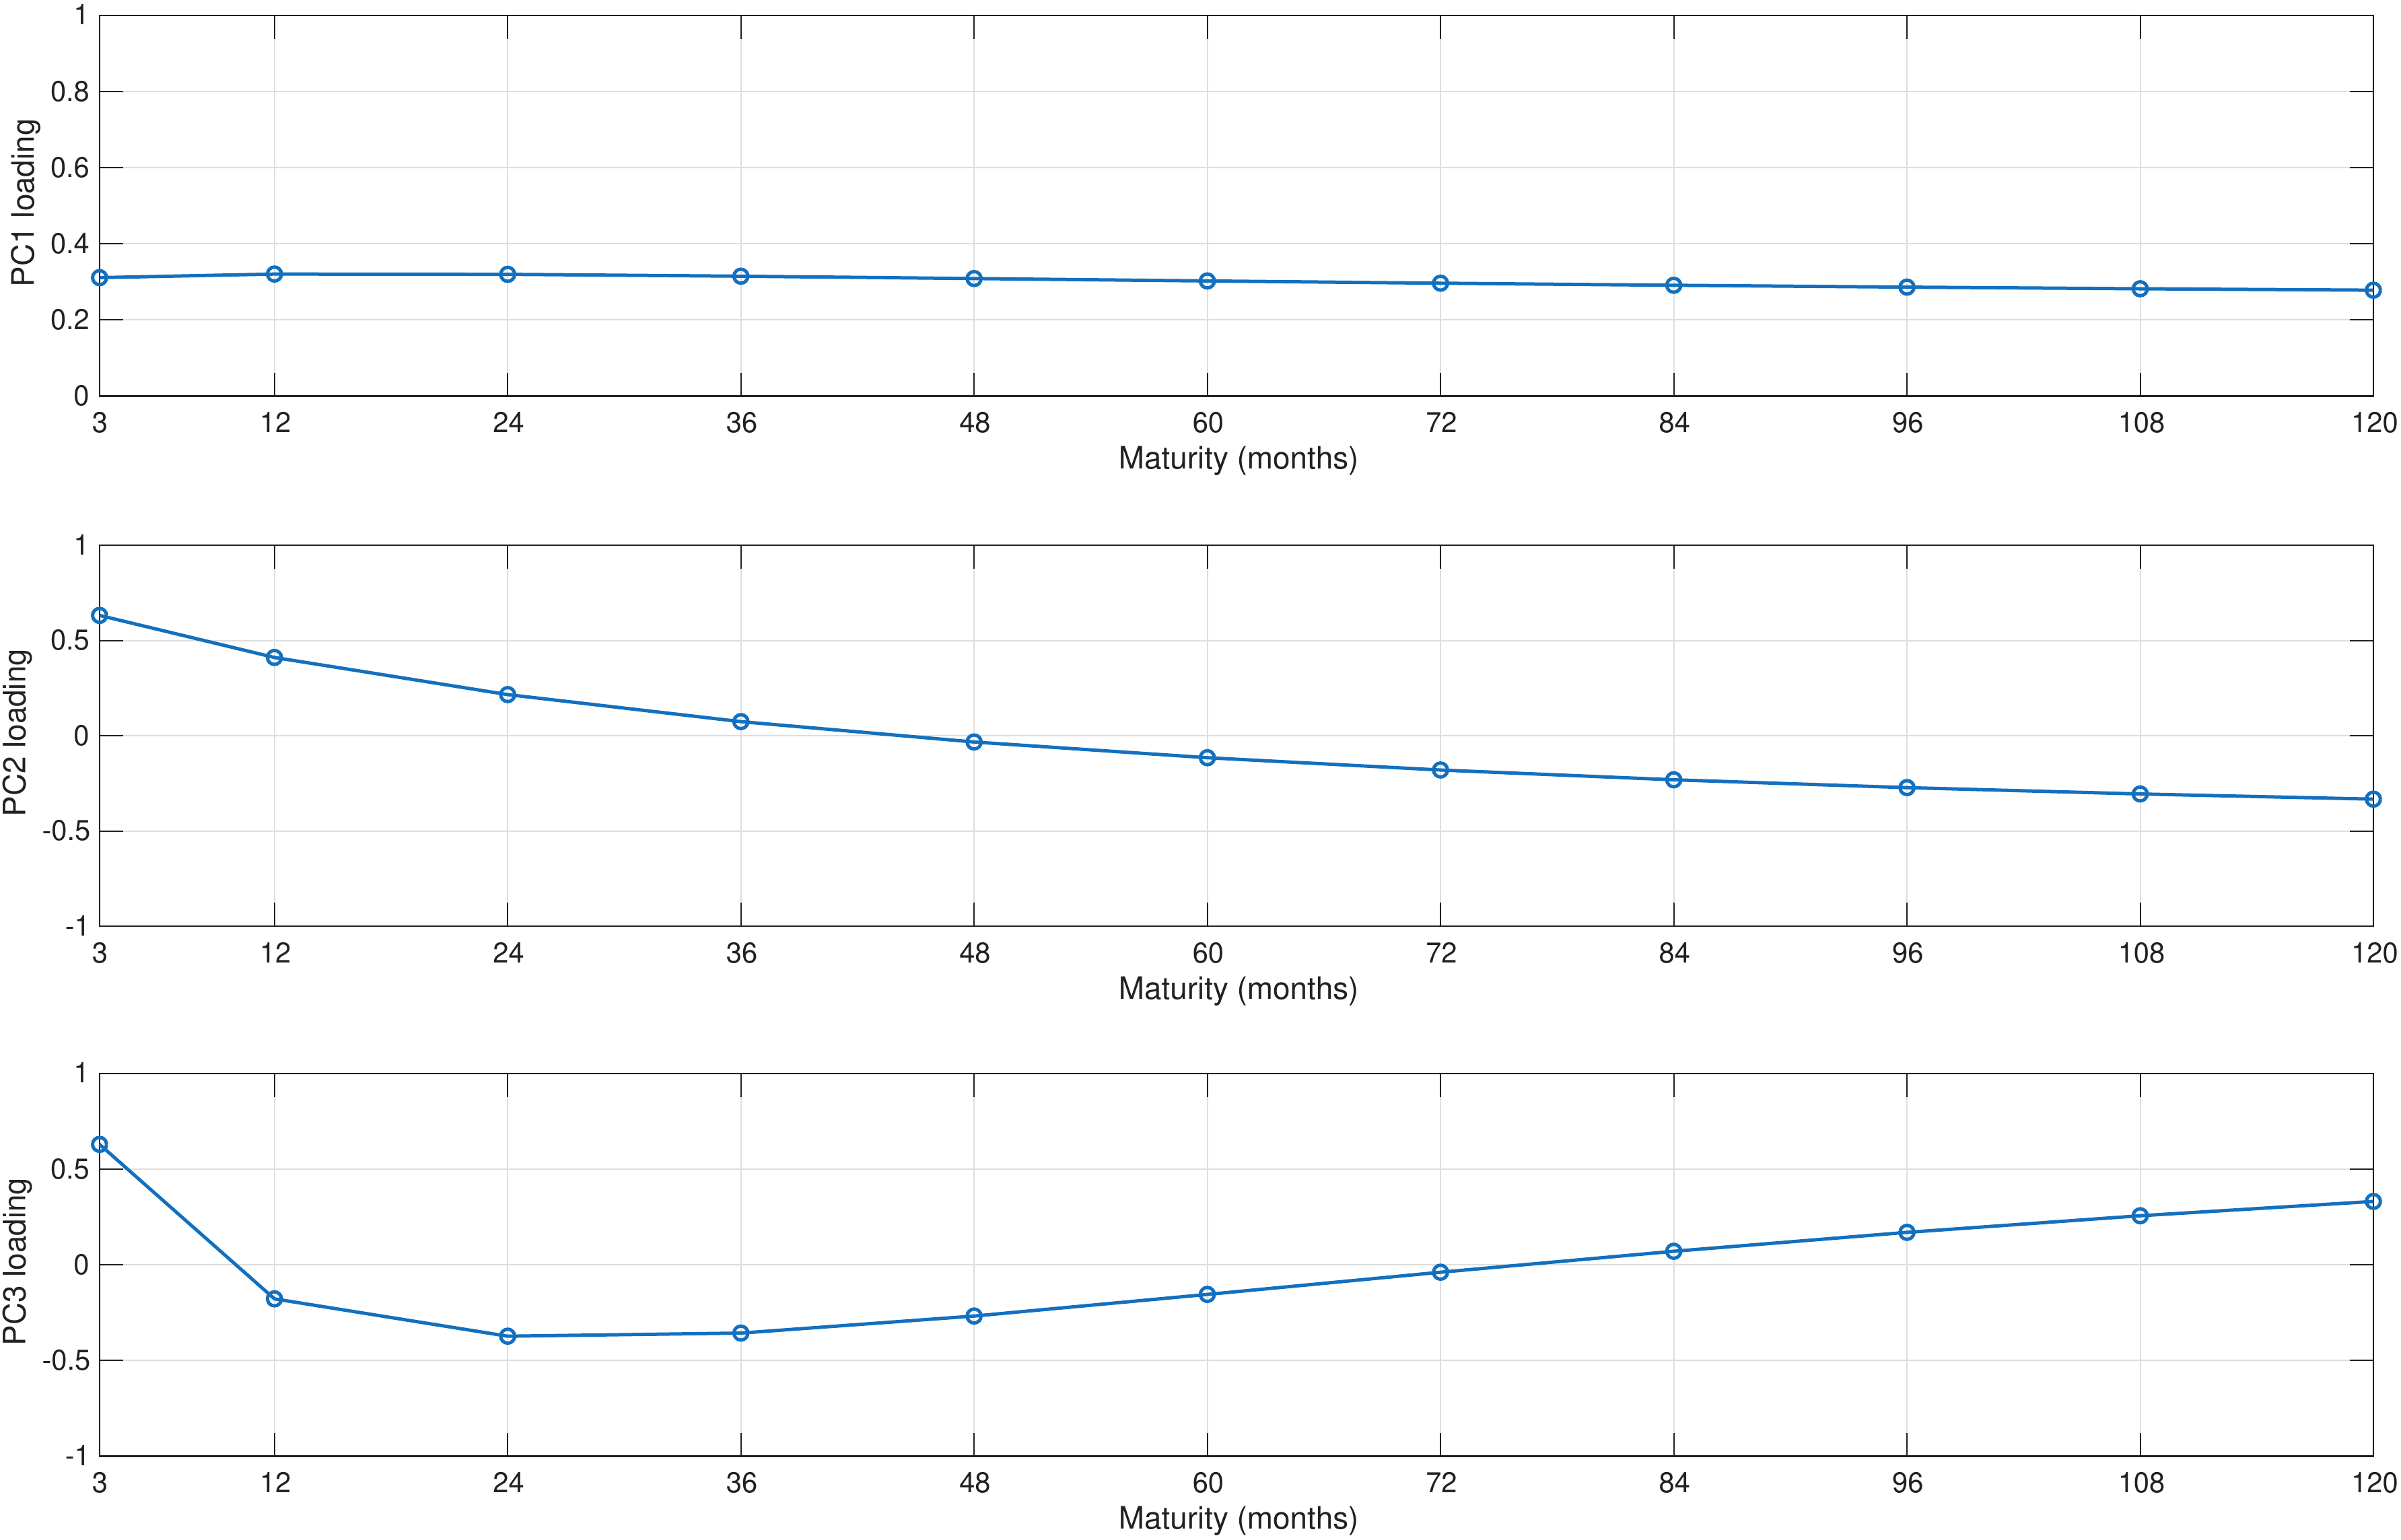
\includegraphics[width=0.85\linewidth,height=\textheight,keepaspectratio]{img/PC_loadings.png}

}

\caption{\label{fig-PCA-loadings}Cross--sectional loadings of the first
three principal components}

\end{figure}%

\emph{The figure shows the loadings of the first three principal
components extracted from monthly US Treasury yields across maturities
from 3 to 120 months. The first component loads roughly equally on all
maturities, the second loads more strongly on short maturities than on
long ones, and the third exhibits a hump--shaped pattern.}

\subsection{Time--series behaviour of the PCA
factors}\label{timeseries-behaviour-of-the-pca-factors}

While the loadings describe how each factor affects the cross--section
of yields at a given point in time, the factor scores trace out the
temporal evolution of these effects. Figure~\ref{fig-PCA-factors} plots
the time series of the first three principal components extracted from
the monthly US Treasury yield data over the sample period.

\begin{figure}

\centering{

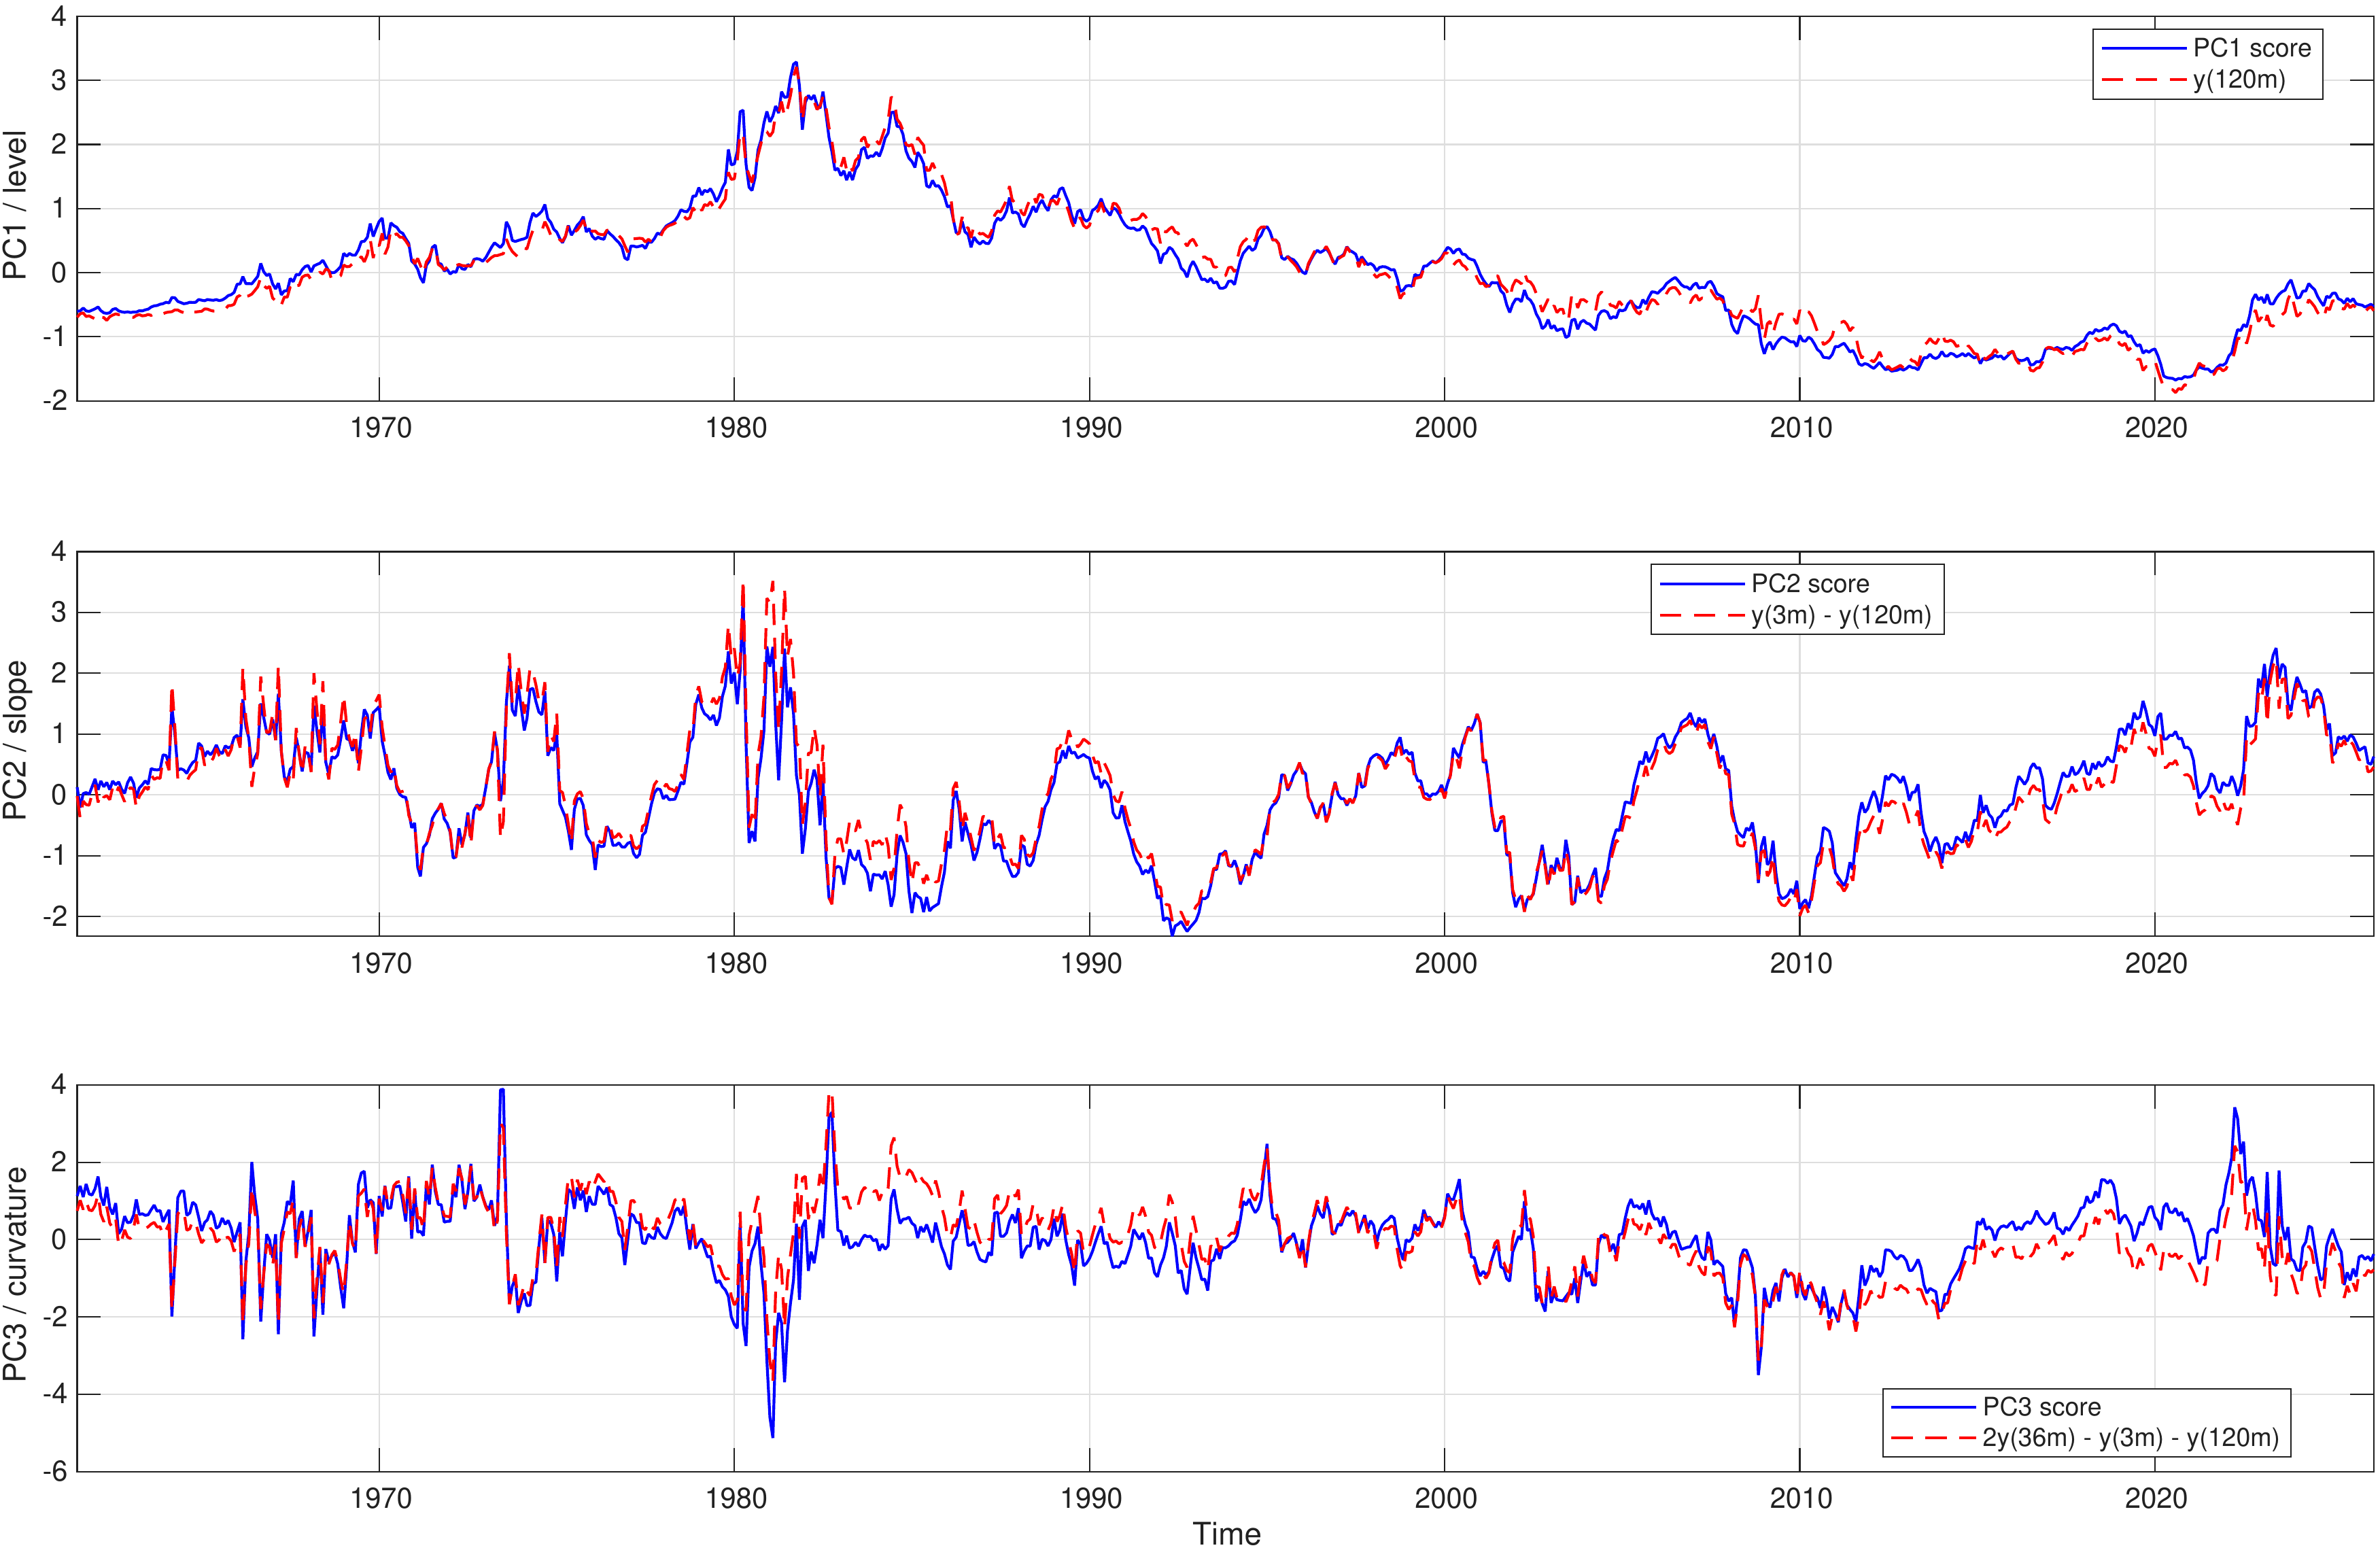
\includegraphics[width=0.85\linewidth,height=\textheight,keepaspectratio]{img/factor_time_series.png}

}

\caption{\label{fig-PCA-factors}Time series of the first three principal
components}

\end{figure}%

\emph{The figure shows the time series of the first three principal
components extracted from monthly US Treasury yields across maturities
from 3 to 120 months over the period 1960--2026, overlaid with simple
empirical proxies. In each panel the solid blue line shows the
standardised PCA score (factor), while the dashed red line shows its
empirical counterpart: the 10‑year yield (level) in the top panel, the
spread between the 3‑month and 10‑year yields (slope) in the middle
panel, and the curvature proxy \(2y(36m) − y(3m) − y(120m)\) in the
bottom panel.}

Figure~\ref{fig-PCA-factors} shows the time--series behaviour of the
first three principal components extracted from the panel of monthly US
Treasury yields together with simple, economically motivated
yield--curve measures. Each panel plots a standardised PCA score (solid
blue line) and the empirical counterpart constructed directly from the
yields (dashed red line). The purpose of this comparison is to show that
the statistically extracted components have a very natural
interpretation as observable quantities.

In the top panel the first principal component is overlaid with the
10‑year yield, taken as a proxy for the overall level of the term
structure. The close co--movement of the two series confirms that the
first component primarily tracks the general interest rate environment:
both spike during the high‑inflation episode of the late 1970s and early
1980s, decline during the subsequent disinflation, and remain low in the
post‑crisis period. This visual evidence reinforces the interpretation
of the first component as a level factor.

The middle panel compares the second principal component with the spread
between the 3‑month and 10‑year yields. This spread is a standard
measure of yield--curve slope and encapsulates the relative pricing of
short‑ and long‑term interest rates. The fact that the PCA score and the
empirical slope proxy move almost one--for--one, including during
episodes of curve steepening and inversion, indicates that the second
component captures slope movements in the term structure. It therefore
refines the purely parallel picture suggested by the level factor by
allowing for differential shifts between the front and the back end of
the curve.

The bottom panel shows the third principal component together with a
curvature proxy defined as
\begin{align}
2 \cdot y(36\text{m}) - y(3\text{m}) - y(120\text{m}), \nonumber
\end{align}
which measures the extent to which medium‑term yields deviate from the
average of short‑ and long‑term yields. Periods in which this proxy is
high correspond to yield curves that are relatively elevated at
intermediate maturities (hump--shaped), whereas low values indicate
curves that are depressed in the middle (inverse hump). The strong
alignment between the third PCA score and this curvature measure shows
that the third component captures precisely these curvature
fluctuations.

\subsection{PCA as a static factor model and its state--space
representation}\label{pca-as-a-static-factor-model-and-its-statespace-representation}

The PCA decomposition can be viewed as a static factor model for the
yield curve. Let \(y_t\) denote the \(k\times 1\) vector of de--meaned
yields at time \(t\), stacked across maturities. Collecting the first
\(r\) principal components in the \(k\times r\) loading matrix
\(\Lambda\) (consisting of the first \(r\) columns of \(L\)), and the
corresponding factor scores in the \(r\times 1\) vector \(f_t\), the PCA
representation for \(y_t\) can be written as
\begin{equation}\protect\phantomsection\label{eq-PCA-obs-equation}{
\begin{align}
    y_t &= \Lambda f_t + \varepsilon_t,
\end{align}
}\end{equation} where \(\varepsilon_t\) is a \(k\times 1\) vector of
idiosyncratic residuals that are orthogonal to the factors by
construction. In the exact reconstruction case discussed above the model
is estimated with \(r=k\) and \(\varepsilon_t\equiv 0\); in practice one
typically retains only the first \(r\ll k\) components (for example
\(r=3\)), in which case \(\varepsilon_t\) collects the small amount of
variation not explained by the retained factors.

To move towards a dynamic term--structure model, we now endow the factor
vector \(f_t\) with its own stochastic law of motion. The simplest and
most widely used specification is a first--order vector autoregression,
\begin{equation}\protect\phantomsection\label{eq-PCA-state-equation}{
\begin{align}
    f_{t+1} &= \Phi f_t + \eta_{t+1},
\end{align}
}\end{equation} where \(\Phi\) is an \(r\times r\) coefficient matrix
and \(\eta_{t+1}\) is an \(r\times 1\) innovation with zero mean and
covariance matrix \(Q\). Together, the observation
equation~Equation~\ref{eq-PCA-obs-equation} and the state
equation~Equation~\ref{eq-PCA-state-equation} define a linear Gaussian
state--space model for the yield curve, with the principal components
serving as latent state variables.

This state--space representation provides a natural bridge from static
PCA to fully dynamic yield--curve models. The PCA step identifies the
dominant cross--sectional factors and their loadings, while the state
equation specifies how these factors evolve over time. In subsequent
chapters we will replace the reduced--form dynamics above by more
structured specifications motivated by no--arbitrage and
macro--financial considerations, but the underlying
level--slope--curvature factor structure revealed by PCA will remain at
the core of those models.

\section[A recipe for building term-structure models]{\texorpdfstring{A
recipe for building term-structure
models\footnote{See also Nyholm (2021)}}{A recipe for building term-structure models}}\label{a-recipe-for-building-term-structure-models9}

Virtually all Gaussian dynamic term-structure models can be built by
following a relatively mechanical sequence of steps that has emerged
from the affine term-structure literature, see, for example, Duffie and
Kan (1996), Dai and Singleton (2000), and Ang and Piazzesi (2003). In
this section, we stay with discrete-time models, which means that the
factor dynamics are specified as vector autoregressions rather than
continuous-time diffusions, and that sums, instead of integrals, are
used in all pricing expressions.

Let \(X_t\) denote the vector of the modelled yield curve factors, at
time \(t\), and let the dynamics of \(X_t\) be governed by vector
autoregressive (VAR) processes of order one, under both the empirical
measure, \(\mathbb{P}\), and the pricing measure, \(\mathbb{Q}\):
\begin{equation}\protect\phantomsection\label{eq-factorVarP}{
\begin{align}
    X_{t} &= k^\mathbb{P}+\Phi^\mathbb{P} \cdot X_{t-1} + \Sigma^{\mathbb{P}} \epsilon^\mathbb{P}_{t}, \hspace{1cm} \epsilon^\mathbb{P}_{t} \sim N(0,1)  
\end{align}
}\end{equation}

\begin{equation}\protect\phantomsection\label{eq-factorVarQ}{
\begin{align}
    X_{t} &= k^\mathbb{Q}+\Phi^\mathbb{Q} \cdot X_{t-1} +\Sigma^{\mathbb{Q}} \epsilon^\mathbb{Q}_{t}, \hspace{1cm} \epsilon^\mathbb{Q}_{t} \sim N(0,1).
\end{align}
}\end{equation} with \(\Sigma \Sigma^{\top}=\Omega\) being the variance
of the residuals, and it is assumed that
\(\Sigma^{\mathbb{P}}=\Sigma^{\mathbb{Q}}\). \(\Phi^{\mathbb{Q}}\) is a
core element since it is responsible for the mapping of unobserved
factors into observed yields. In the PCA section above,
\(\Phi^{\mathbb{Q}}\) corresponds to the matrix of loadings \(\Lambda\)
in Equation~\ref{eq-PCA-obs-equation}. If a closed form expression for
the loading structure is desirable, and if a certain economic
interpretation should be imposed on the factors in the model, then this
is done through the parametrisation of \(\Phi^{\mathbb{Q}}\). For
example, to obtain the loadings for the dynamic Nelson-Siegel model
(see, Christensen et al. (2011)) the following specification is used:
\begin{align}
    \Phi^{\mathbb{Q}} = \begin{bmatrix}  0 & 0 & 0\\
                                          0 & \lambda & -\lambda \\
                                            0 & 0 & \lambda  \end{bmatrix}
\end{align}
For the pricing of assets (here bonds) we need an expression for the
one-period short rate. It is assumed that the short rate is found as a
linear combination of the yield curve factors collected in \(X_t\), so
we have that:
\begin{equation}\protect\phantomsection\label{eq-shortRate}{
\begin{align}
    r_t = \rho_0 + \rho^{\top}_1 X_t.
\end{align}
}\end{equation}

To impose absence of arbitrage we impose the unique pricing mechanism,
that governs all traded assets:
\begin{equation}\protect\phantomsection\label{eq-noArbitrage}{
\begin{align}
    P_{t,n} = \mathbb{E}_t \left[ M_{t+1}\cdot P_{t+1,n-1} \right]
\end{align}
}\end{equation} The idea here is that when the bond matures at time
\(T\), its value is known with certainty, since it is default-free: the
bond pays its principal value on that day, so \(P_{T,0}=1\). At any time
\(t+j\) before maturity, the price of the bond can therefore be found as
the one-period discounted-value of the price at time \(t+j+1\), all the
way back to time \(t\). Discounting is done using the stochastic
discount factor (also called the pricing kernel), which is denoted by
\(M_t\), and this quantity is assumed to be given by:
\begin{equation}\protect\phantomsection\label{eq-kernel}{
\begin{align} 
    M_{t+1} = \text{exp}\left( -r_t -\frac{1}{2} \lambda^{\top}_t \lambda_t - \lambda^{\top}_t \epsilon^\mathbb{P}_{t+1} \right)
\end{align}
}\end{equation} with the market price of risk (as above) given by:
\begin{align}
    \lambda_t = \lambda_0 + \lambda_1 \cdot X_t,
\end{align}

It is recalled that:
\begin{align}
    y_{t,n} = -\frac{1}{n}\text{log}(P_{t,n}),
\end{align}
and that we can write the yield curve expression as an affine function
(note that contrary to Chapter 0, here we define the yield equation with
\(-A_n\) and \(-B_n\), as this is common in the literature, i.e.~a
minus-sign is included for \(A\) and \(B\)):
\begin{equation}\protect\phantomsection\label{eq-yield}{
\begin{align}
    y_{t,n} = -\frac{A_{n}}{n} - \frac{B^{\top}_{n}}{n} X_t.
\end{align}
}\end{equation} The bond price is therefore exponential affine in terms
of \(A_{n}\) and \(B_{n}\):
\begin{equation}\protect\phantomsection\label{eq-Pt1}{
\begin{align}
    P_{t,n} = \text{exp} \left( A_{n} + B^{\top}_{n} X_t \right).
\end{align}
}\end{equation} To derive closed-form expressions for \(A_{n}\) and
\(B_{n}\), the fundamental pricing equation is invoked
Equation~\ref{eq-kernel}:
\begin{align}
    P_{t,n} &= \mathbb{E}_t\left[ M_{t+1} \cdot P_{t+1,n-1} \right] \\
               &= \mathbb{E}_t \left[ \text{exp}\left( -r_t -\frac{1}{2} \lambda^{\top}_t\lambda_t - \lambda^{\top}_t \epsilon^\mathbb{P}_{t+1} \right) \cdot \text{exp}\left( A_{n-1} + B^{\top}_{n-1} X_{t+1} \right) \right].
\end{align}
The expression for \(X_{t+1}\) (see equation
Equation~\ref{eq-factorVarP}) is substituted:
\begin{align}
    P_{t,n} = \mathbb{E}_t \left[ \text{exp}\left( -r_t -\frac{1}{2} \lambda^{\top}_t \lambda_t - \lambda^{\top}_t \epsilon^\mathbb{P}_{t+1} \right) \cdot \text{exp}\left( A_{n-1} + B^{\top}_{n-1} \left( k^\mathbb{P}+\Phi^\mathbb{P} X_{t} + \Sigma \epsilon^\mathbb{P}_{t+1} \right) \right) \right],
\end{align}
and, the terms are then separated into two groups: one to which the
expectations operator should be applied, i.e.~\(t+1\) terms, and another
group, which are known at time \(t\):
\begin{equation}\protect\phantomsection\label{eq-PtIntermed}{
\begin{align}
    P_{t,n} = &\text{exp}\left( -r_t - \frac{1}{2} \lambda^{\top}_t \lambda_t + A_{n-1} + B^{\top}_{n-1} k^{\mathbb{P}} +B^{\top}_{n-1} \Phi^\mathbb{P} X_{t} \right) \nonumber \\ 
    \cdot &\mathbb{E}_t\left[ \text{exp}\left( -\lambda^{\top}_t \epsilon^{\mathbb{P}}_{t+1} + B^{\top}_{n-1} \Sigma \epsilon^\mathbb{P}_{t+1} \right)  \right].
\end{align}
}\end{equation} The question is then, how can we calculate the
expectations part of Equation~\ref{eq-PtIntermed}:
\begin{align}
    \mathbb{E}_t \left[ \text{exp}\left( -\lambda^{\top}_t + B^{\top}_{n-1} \Sigma \right) \epsilon^\mathbb{P}_{t+1}  \right].
\end{align}
To this end, the moment generating function of the multivariate normal
distribution is used. Since \(\epsilon^\mathbb{P} \sim N(0,I)\), it is
known that:
\begin{align}
    \mathbb{E}[\text{exp}(a^{\top}\epsilon^\mathbb{P})] = \text{exp}\left( \frac{1}{2} a^{\top} \cdot I \cdot a  \right),
\end{align}
so, the expectation in Equation~\ref{eq-PtIntermed} can be calculated,
using \(a^{\top}=( -\lambda^{\top}_t + B^{\top}_{n-1} \Sigma )\), as:
\begin{align}
     &\text{exp} \left[ \frac{1}{2} ( -\lambda^{\top}_t + B^{\top}_{n-1} \Sigma ) \cdot I \cdot ( -\lambda^{\top}_t + B^{\top}_{n-1} \Sigma )^{\top}  \right] \nonumber \\
    = &\text{exp} \left[ \frac{1}{2} ( -\lambda^{\top}_t + B^{\top}_{n-1} \Sigma ) \cdot I \cdot ( -\lambda_t + \Sigma^{\top} B_{n-1} ) \right] \nonumber \\
    = &\text{exp} \left[ \frac{1}{2} \left( \lambda^{\top}_t \lambda_t - \lambda^{\top}_t\Sigma^{\top} B_{n-1} - B^{\top}_{n-1} \Sigma \lambda_t + B^{\top}_{n-1} \Sigma \Sigma^{\top} B_{n-1} \right) \right],
\end{align}
and, since \(B^{\top}_{n-1} \Sigma \lambda_t\) is a scalar, and for a
scalar \(h\), we know that \(h=h^{\top}\), so
\(B^{\top}_{n-1} \Sigma \lambda_t = \lambda^{\top}_t \Sigma^{\top} B_{n-1}\).
We can then write:
\begin{align}
    &\mathbb{E}_t \left[ \text{exp}\left( -\lambda^{\top}_t + B^{\top}_{n-1} \Sigma  \right)   \epsilon^\mathbb{P}_{t+1}  \right] \nonumber \\ 
    = &\text{exp}\left[  \left( \frac{1}{2} \lambda^{\top}_t \lambda_t - B^{\top}_{n-1} \Sigma \lambda_t + \frac{1}{2} B^{\top}_{n-1} \Sigma \Sigma^{\top} B^{\top}_{n-1} \right) \right].
\end{align}
This term is then reinserted into Equation~\ref{eq-PtIntermed}, giving:
\begin{equation}\protect\phantomsection\label{eq-Pt2}{
\begin{align}
    P_{t,n} = \text{exp}\left( -r_t + A_{n-1} + B^{\top}_{n-1} k^\mathbb{P} +B^{\top}_{n-1} \Phi^\mathbb{P} X_{t} - B^{\top}_{n-1} \Sigma \lambda_t + \frac{1}{2} B^{\top}_{n-1} \Sigma \Sigma^{\top} B^{\top}_{n-1} \right).
\end{align}
}\end{equation} It is recalled that \(r_t=\rho^{\top}_1 X_t\), and that
\(\lambda_t = \lambda_0 + \lambda_1 X_t\). Inserting these expressions
into Equation~\ref{eq-Pt2}, gives:
\begin{align}
    P_{t,n} = \text{exp} \Big( -&\rho^{\top}_1 X_t + A_{n-1} + B^{\top}_{n-1} k^\mathbb{P} +B^{\top}_{n-1} \Phi^\mathbb{P} X_{t} \nonumber \\
     - &B^{\top}_{n-1} \Sigma \left(\lambda_0 + \lambda_1 X_t \right) + \frac{1}{2} B^{\top}_{n-1} \Sigma \Sigma^{\top} B^{\top}_{n-1} \Big).
\end{align}
Reorganising this expression into terms that load on \(X_t\) and terms
that do not, help matching coefficients with respect to equation
Equation~\ref{eq-Pt1}:
\begin{align}
    P_{t,n} = \text{exp}\Big( A_{n-1} + B^{\top}_{n-1} \left( k^\mathbb{P} - \Sigma \lambda_0 \right) + \frac{1}{2} B^{\top}_{n-1} \Sigma \Sigma^{\top} B^{\top}_{n-1} \nonumber  \\ 
      +  B^{\top}_{n-1} \Phi^\mathbb{P} X_{t} -\rho^{\top}_1 X_t - B^{\top}_{n-1} \Sigma \lambda_1 X_t \Big),
\end{align}
which is: \begin{equation}\protect\phantomsection\label{eq-PtFinal}{
\begin{align}
    P_{t,n} = \text{exp}\Bigg( A_{n-1} + B^{\top}_{n-1} \left( k^\mathbb{P} - \Sigma \lambda_0 \right) + \frac{1}{2} B^{\top}_{n-1} \Sigma \Sigma^{\top} B^{\top}_{n-1} \nonumber  \\ 
      +  \left[ B^{\top}_{n-1} \left( \Phi^\mathbb{P}- \Sigma \lambda_1 \right) - \rho^{\top}_1 \right] X_t \Bigg).
\end{align}
}\end{equation} Matching the coefficients of Equation~\ref{eq-PtFinal}
with those of Equation~\ref{eq-Pt1} establishes the recursive formulas
for \(A_{n}\) and \(B_{n}\):
\begin{equation}\protect\phantomsection\label{eq-Bfin}{
\begin{align}
    A_n  &= A_{n-1} + B^{\top}_{n-1} k^\mathbb{Q} +\frac{1}{2} B^{\top}_{n-1} \Sigma \Sigma^{\top} B^{\top}_{n-1} \\
    B^{\top}_n &= B^{\top}_{n-1} \Phi^\mathbb{Q} - \rho^{\top}_1
\end{align}
}\end{equation} with \(k^\mathbb{Q} = k^\mathbb{P} - \Sigma \lambda_0\),
and \(\Phi^\mathbb{Q} =  \Phi^\mathbb{P}- \Sigma \lambda_1\). Using
recursive substitution, we realise that the expression for
\(B^{\top}_n\) also can be written in the following way:\footnote{We see
  this through an example. For \(n=3\), we have:
  \begin{align}
      B^{\top}_1 &= -\rho^{\top}_1 \nonumber \\
      B^{\top}_2 &= B^{\top}_1 \Phi^\mathbb{Q} - \rho^{\top}_1 = -\rho^{\top}_1 \Phi^\mathbb{Q} - \rho^{\top}_1 \nonumber \\
      B^{\top}_3 &= B^{\top}_2 \Phi^\mathbb{Q} - \rho^{\top}_1 = (-\rho^{\top}_1 \Phi^\mathbb{Q} - \rho^{\top}_1) \Phi^\mathbb{Q} - \rho^{\top}_1 \nonumber \\
       &= -\rho^{\top}_1 \left(\Phi^\mathbb{Q}\right)^2 - \rho^{\top}_1 \Phi^\mathbb{Q} - \rho^{\top}_1 \nonumber \\
       &= -\rho^{\top}_1 \left(  \left(\Phi^\mathbb{Q}\right)^2 + \left(\Phi^\mathbb{Q}\right)^1 + \left(\Phi^\mathbb{Q}\right)^0    \right) \nonumber \\
       &= -\rho^{\top}_1 \left[  \sum_{k=0}^2\left( \Phi^\mathbb{Q} \right)^k \right] \nonumber
       %      \text{so,} \nonumber \\
      %  B_3&= -\left[  \sum_{k=0}^2\left( \Phi^\mathbb{Q} \right)^k \right]^{\top} \rho_1, \nonumber
  \end{align}
  which generalises to equation Equation~\ref{eq-Bn-recur-final}.}
\begin{equation}\protect\phantomsection\label{eq-Bn-recur-final}{
\begin{align}
    B^{\top}_{n} = -\rho^{\top}_1 \, \left[ \sum_{k=0}^{n-1}\left( \Phi^\mathbb{Q} \right)^k \right].
\end{align}
}\end{equation} The sum in the expression for \(B_n\) in
Equation~\ref{eq-Bn-recur-final} is the multivariate analogue of the
scalar geometric sum in Equation~\ref{eq-Bn}. In matrix form, and
whenever the corresponding geometric matrix series is well defined, we
have: \begin{equation}\protect\phantomsection\label{eq-Bn-final}{
\begin{align}
    B_n^{\top} = -\rho_1^{\top} \left[ \sum_{k=0}^{n-1} \left( \Phi^{\mathbb{Q}} \right)^k \right] 
               = -\rho_1^{\top} \left[ \left( I - \left( \Phi^{\mathbb{Q}} \right)^n \right) \left( I - \Phi^{\mathbb{Q}} \right)^{-1} \right],
\end{align}
}\end{equation} which is the matrix version of the finite geometric sum.
This naturally only holds when \(I - \Phi^{\mathbb{Q}}\) is invertible.

If \(I - \Phi^{\mathbb{Q}}\) is not invertible, the geometric-series
cannot be used directly, and we can instead rely on the Jordan
decomposition (as \(\Phi^{\mathbb{Q}}\) is guaranteed to be a square
matrix):
\begin{align}
    \Phi^{\mathbb{Q}} = S J S^{-1},
\end{align}
with \(J\) in Jordan normal form, and powers given by:
\begin{align}
    \left(\Phi^{\mathbb{Q}}\right)^n = S J^n S^{-1}.
\end{align}
which leads to:
\begin{align}
    \sum_{k=0}^{n-1} \left( \Phi^{\mathbb{Q}} \right)^{k}
        = S \left( \sum_{k=0}^{n-1} J^{k} \right) S^{-1}
\end{align}
and finally to:
\begin{align}
B_n^{\top}
= -\rho_1^{\top} S \left( \sum_{k=0}^{n-1} J^{k} \right) S^{-1}.
\end{align}

The constant term in the exponential-affine bond price is determined by
the recursion for \(A_n\),
\begin{align}
A_n = A_{n-1} + B_{n-1}^{\top} k^{\mathbb{Q}} 
      + \frac{1}{2} B_{n-1}^{\top} \Sigma \Sigma^{\top} B_{n-1},
\end{align}
which aggregates contributions from the risk-neutral drift
\(k^{\mathbb{Q}}\) and the conditional variance \(\Sigma \Sigma^{\top}\)
over the maturity dimension. This demonstrate that the real difference
between models that exclude arbitrage by construction, and those that do
not, for example the dynamic Nelson-Siegel models, is whether the
constant \(A_n\) is included in the model or not.

\bookmarksetup{startatroot}

\chapter{Implementation and
estimation}\label{implementation-and-estimation}

In this section we move from model construction to model implementation
and estimation. Up to this point, the focus has been on specifying
factor dynamics and enforcing absence of arbitrage in a general affine
setting. For estimation, however, it is useful to be explicit about how
we parameterise the relationship between factors, bond prices and
yields. Two equivalent but notationally distinct conventions will be
used throughout this chapter: a \emph{price--affine} representation and
a \emph{yield--affine} representation.

In the \textbf{price--affine} convention, zero--coupon bond prices are
written as exponential--affine functions of the state vector,
\begin{align}
P_{t,n} &= \exp\!\big( A_n^{(P)} + B_n^{(P)\prime} X_t \big),
\end{align}
and yields are defined from prices via
\begin{align}
y_{t,n}
&= - \frac{1}{n} \log P_{t,n}
 \;=\; -\frac{1}{n}\big( A_n^{(P)} + B_n^{(P)\prime} X_t \big).
\end{align}
In this parametrisation the affine recursions derived earlier directly
deliver the \emph{price} coefficients \(A_n^{(P)}\) and \(B_n^{(P)}\),
while the minus sign in the mapping from prices to yields is carried
explicitly in the yield equation. This convention is standard in the
affine term--structure literature and provides a convenient starting
point for linking factor dynamics under the pricing measure
\(\mathbb{Q}\) to no--arbitrage restrictions on bond prices.

In the \textbf{yield--affine} convention, we instead parameterise yields
directly as affine functions of the state,
\begin{align}
y_{t,n}
&= \frac{1}{n}\big( A_n^{(Y)} + B_n^{(Y)\prime} X_t \big),
\end{align}
so that bond prices are obtained as
\begin{align}
P_{t,n}
&= \exp\!\big( - A_n^{(Y)} - B_n^{(Y)\prime} X_t \big).
\end{align}
Here \(A_n^{(Y)}\) and \(B_n^{(Y)}\) can be interpreted directly as
yield loadings and are often more transparent from an economic point of
view, especially in models such as Nelson--Siegel or the terminal rate
specification, where the factor loadings are designed to have a
particular shape across maturities.

As shown in the previous section, these two parametrisations are
algebraically equivalent. Matching prices and yields for all states
\(X_t\) implies the simple mapping
\begin{align}
A_n^{(Y)} &= - A_n^{(P)}, \\
B_n^{(Y)} &= - B_n^{(P)}.
\end{align}
The choice between them is therefore purely a matter of convenience and
interpretation: the underlying model, its dynamics under \(\mathbb{P}\)
and \(\mathbb{Q}\), and its implied prices and yields are unchanged.

In what follows, this equivalence will be exploited in a systematic way.
For the \emph{implementation and estimation} of the
Joslin--Singleton--Zhu (JSZ) (Joslin et al. 2011) canonical framework we
work primarily with the price--affine representation, since it aligns
naturally with their decomposition of the \(\mathbb{Q}\)--dynamics and
with the separation of cross--sectional and time--series parameters. For
the affine Nelson--Siegel (AFNS) and terminal rate (TRM) models, by
contrast, we will report both the price--affine coefficients produced by
the general recursion and the corresponding yield--affine loadings that
connect directly to the familiar level--slope--curvature and
terminal--rate interpretations. Throughout this section, references back
to the general derivations in the previous section will make explicit
when we are working in the price--affine or yield--affine convention,
and how to move between them when estimating and comparing models.

\section{Dynamic Nelson-Siegel}\label{dynamic-nelson-siegel}

The affine Nelson--Siegel (AFNS) model of Christensen et al. (2011)
provides an arbitrage--free counterpart to the dynamic Nelson--Siegel
(DNS) model (Diebold and Li 2006) while preserving its familiar
level--slope--curvature interpretation. In this section we formulate
AFNS in the discrete--time Gaussian framework introduced above and show
how it fits into the general ``recipe'' of Section~2.2.

\subsection*{Yield representation and state
vector}\label{yield-representation-and-state-vector}
\addcontentsline{toc}{subsection}{Yield representation and state vector}

The starting point is the Nelson--Siegel yield representation for a
given maturity \(n\) (or, equivalently, maturity
\(\tau_n = n \Delta t\)):
\begin{align}
y_{t,n}
&= L_t
+ S_t \, f_2(\tau_n)
+ C_t \, f_3(\tau_n),
\end{align}
where
\begin{align}
f_2(\tau) &= \frac{1 - e^{-\lambda \tau}}{\lambda \tau}, \\
f_3(\tau) &= \frac{1 - e^{-\lambda \tau}}{\lambda \tau}
            - e^{-\lambda \tau},
\end{align}
and the latent factors \(L_t\), \(S_t\), \(C_t\) are interpreted as
level, slope, and curvature. Let
\begin{align}
X_t
&=
\left[
\begin{array}{c}
L_t \\
S_t \\
C_t
\end{array}
\right],
\end{align}
and define the maturity--specific loading vector
\begin{align}
B_n^{(Y)}
&=
\left[
\begin{array}{c}
\tau_n \\
\tau_n f_2(\tau_n) \\
\tau_n f_3(\tau_n)
\end{array}
\right].
\end{align}
Then the yield at time \(t\) and maturity \(n\) can be written compactly
as \begin{equation}\protect\phantomsection\label{eq-AFNS-yield}{
\begin{align}
y_{t,n}
&= \frac{1}{\tau_n} \, B_n^{(Y)\prime} X_t.
\end{align}
}\end{equation} This is a \emph{yield--affine} representation: the
loadings \(B_n^{(Y)}\) are directly the Nelson--Siegel factor--loading
functions multiplied by maturity, and they carry the intuitive
level--slope--curvature signs.

\subsection*{Risk--neutral dynamics and short
rate}\label{riskneutral-dynamics-and-short-rate}
\addcontentsline{toc}{subsection}{Risk--neutral dynamics and short rate}

To embed this representation in an arbitrage--free affine
term--structure model, we specify discrete--time \(Q\)--measure dynamics
for the factors as a first--order VAR:
\begin{equation}\protect\phantomsection\label{eq-AFNS-Q-VAR}{
\begin{align}
X_t &= k^Q + \Phi^Q X_{t-1} + \Sigma \varepsilon_t^Q,
\qquad \varepsilon_t^Q \sim N(0,I_3),
\end{align}
}\end{equation} with the AFNS choice
\begin{equation}\protect\phantomsection\label{eq-AFNS-PhiQ}{
\begin{align}
\Phi^Q
&=
\left[
\begin{array}{ccc}
0 & 0       & 0      \\
0 & \lambda & -\lambda \\
0 & 0       & \lambda
\end{array}
\right].
\end{align}
}\end{equation} Under this specification, the level factor is a pure
random walk under \(Q\), while the slope and curvature factors follow a
bivariate AR(1) system that reproduces the Nelson--Siegel loading
structure in the cross--section.

Following the general recipe, the one--period short rate is assumed to
be an affine function of the factors,
\begin{align}
r_t &= \rho_0 + \rho_1^\prime X_t.
\end{align}
In AFNS it is natural to identify the short rate with the instantaneous
(or shortest--maturity) yield, which, in the Nelson--Siegel limit
\(\tau \to 0\), depends only on level and slope. In the discrete--time
set--up we implement this by setting
\begin{align}
\rho_0 &= 0, \\
\rho_1
&=
\left[
\begin{array}{c}
1 \\
1 \\
0
\end{array}
\right],
\end{align}
so that
\begin{equation}\protect\phantomsection\label{eq-AFNS-short-rate}{
\begin{align}
r_t &= L_t + S_t.
\end{align}
}\end{equation} This choice ensures that for very short maturities the
yield curve coincides with the short rate, while the curvature factor
affects only medium and longer maturities through the Nelson--Siegel
hump.

\subsection*{Exponential--affine bond
prices}\label{exponentialaffine-bond-prices}
\addcontentsline{toc}{subsection}{Exponential--affine bond prices}

As in Section~2.2, we assume that zero--coupon bond prices take the
exponential--affine form
\begin{equation}\protect\phantomsection\label{eq-AFNS-price}{
\begin{align}
P_{t,n}
&= \exp \left( A_n^{(P)} + B_n^{(P)\prime} X_t \right),
\end{align}
}\end{equation} with \(A_0^{(P)} = 0\) and \(B_0^{(P)} = 0\). Yields are
defined by \(P_{t,n} = \exp(- y_{t,n} \tau_n)\), and hence
\begin{equation}\protect\phantomsection\label{eq-AFNS-yield-from-price}{
\begin{align}
y_{t,n}
&= -\frac{1}{\tau_n} \left( A_n^{(P)} + B_n^{(P)\prime} X_t \right).
\end{align}
}\end{equation} Comparing with the desired Nelson--Siegel representation
Equation~\ref{eq-AFNS-yield}, we see that the AFNS model must satisfy
\begin{align}
B_n^{(Y)} &= - B_n^{(P)}, \\
A_n^{(Y)} &= - A_n^{(P)},
\end{align}
where \(A_n^{(Y)}\) is the constant term in the yield representation.
That is, the \emph{price--affine} coefficients \(A_n^{(P)}\),
\(B_n^{(P)}\) produced by the affine recursion are simply the negative
of the \emph{yield--affine} Nelson--Siegel coefficients. The minus sign
resides in the mapping from prices to yields rather than in the NS
loadings themselves.

Given the short--rate specification Equation~\ref{eq-AFNS-short-rate}
and the \(Q\)--VAR Equation~\ref{eq-AFNS-Q-VAR}, the affine pricing
recursion of Section~2.2 applies directly:
\begin{equation}\protect\phantomsection\label{eq-AFNS-A-recursion}{
\begin{align}
A_n^{(P)}
&= A_{n-1}^{(P)} + B_{n-1}^{(P)\prime} k^Q
    + \frac{1}{2} B_{n-1}^{(P)\prime} \Sigma \Sigma^\prime B_{n-1}^{(P)},
\end{align}
}\end{equation}

\begin{equation}\protect\phantomsection\label{eq-AFNS-B-recursion}{
\begin{align}
B_n^{(P)\prime}
&= B_{n-1}^{(P)\prime} \Phi^Q - \rho_1^\prime,
\end{align}
}\end{equation} with \(A_0^{(P)} = 0\) and \(B_0^{(P)} = 0\). In matrix
form, using \(\Phi^Q\) from 1, these recursions can be iterated or
solved in closed form using the geometric--series expressions discussed
in Section~2.2.

For implementation and interpretation, it is often more convenient to
work with the yield--affine NS loadings \(B_n^{(Y)}\). These are
obtained simply as
\begin{equation}\protect\phantomsection\label{eq-AFNS-Byield}{
\begin{align}
B_n^{(Y)} &= - B_n^{(P)},
\end{align}
}\end{equation} and enter the yield equation as
\begin{align}
y_{t,n}
&= \frac{1}{\tau_n} B_n^{(Y)\prime} X_t
= \frac{1}{\tau_n} \left(- B_n^{(P)\prime}\right) X_t.
\end{align}
In other words, the recursive solution from the affine pricing recipe
naturally produces the Nelson--Siegel loadings with the correct sign
structure once we interpret \(B_n^{(Y)} = - B_n^{(P)}\) as the
economically meaningful yield coefficients.

\subsection*{Implementation}\label{implementation}
\addcontentsline{toc}{subsection}{Implementation}

From a computational perspective, AFNS is implemented by:

\begin{enumerate}
\def\labelenumi{\arabic{enumi}.}
\item
  Specifying the risk--neutral dynamics under
  Equation~\ref{eq-AFNS-Q-VAR} with the AFNS matrix \(\Phi^Q\) in

  \begin{enumerate}
  \def\labelenumii{\arabic{enumii}.}
  \tightlist
  \item
  \end{enumerate}
\item
  Setting the short--rate coefficients \(\rho_0\), \(\rho_1\) according
  to Equation~\ref{eq-AFNS-short-rate}.
\item
  Iterating the recursions
  Equation~\ref{eq-AFNS-A-recursion}--Equation~\ref{eq-AFNS-B-recursion}
  up to the maximum maturity of interest to obtain \(A_n^{(P)}\),
  \(B_n^{(P)}\) for all \(n\).
\item
  Constructing the NS yield loadings via Equation~\ref{eq-AFNS-Byield}
  and forming model--implied yields using the yield--affine
  representation \(y_{t,n} = \tau_n^{-1} B_n^{(Y)\prime} X_t\).
\end{enumerate}

\section{Joslin, Singleton, Zhu}\label{joslin-singleton-zhu}

The Gaussian dynamic term structure framework of plays a central role in
the modern affine literature. They show that a wide range of existing
model parametrisations are observationally equivalent---in fact
identical up to a rotation of the state vector---and they provide a
canonical representation in which the estimation of \(\mathbb{P}\)-- and
\(\mathbb{Q}\)--measure parameters becomes particularly transparent.

From the perspective of these notes, the main insights from can be
summarised as follows:

\begin{enumerate}
\def\labelenumi{\arabic{enumi}.}
\item
  Gaussian dynamic term structure models (GDTSMs) can be parameterised
  such that the parameters governing the \(\mathbb{P}\)--measure
  dynamics of the factors \(X_t\) do not appear in the
  measurement--error density. This implies that \(\mathbb{P}\)-- and
  \(\mathbb{Q}\)--measure parameters can be estimated separately.
\item
  No--arbitrage restrictions imposed under \(\mathbb{Q}\) do not feed
  back into the \(\mathbb{P}\)--dynamics of \(X_t\) in this
  parametrisation. Therefore such constraints improve cross--sectional
  fit but, in general, do not improve the forecasting performance of
  GDTSMs.
\item
  For an \(N\)--factor GDTSM, the canonical JSZ representation is fully
  characterised by a small set of economically interpretable objects:

  \begin{enumerate}
  \def\labelenumii{\arabic{enumii}.}
  \item
    \(r^{\mathbb{Q}}_{\infty}\), the long--run mean of the short rate
    under the risk--neutral measure;
  \item
    the \(N\) eigenvalues gathered in \(\gamma^{\mathbb{Q}}\), which
    determine the mean--reversion speeds of the factors under
    \(\mathbb{Q}\);
  \item
    the conditional covariance matrix \(\Sigma^{\mathbb{P}}\) governing
    the VAR dynamics of the factors under \(\mathbb{P}\).
  \end{enumerate}
\item
  The JSZ characterisation is based on the notion of \emph{similar}
  matrices from linear algebra. If the \(\mathbb{Q}\)--dynamics of a
  given GDTSM can be written in Jordan form with ordered eigenvalues,
  then the model is identical (up to a rotation of the state vector) to
  the JSZ canonical form.
\end{enumerate}

\subsection*{\texorpdfstring{Canonical \(\mathbb{Q}\)--dynamics and
rotation}{Canonical \textbackslash mathbb\{Q\}--dynamics and rotation}}\label{canonical-mathbbqdynamics-and-rotation}
\addcontentsline{toc}{subsection}{Canonical \(\mathbb{Q}\)--dynamics and
rotation}

As in , we consider yield curve factors that are linear combinations of
observed yields. Let \(y_t\) denote the \(k\times 1\) vector of yields
at time \(t\), and define
\begin{equation}\protect\phantomsection\label{eq-JSZ-portfolio-factors}{
\begin{align}
X_t &= W y_t,
\end{align}
}\end{equation} for some \(N\times k\) weighting matrix \(W\). JSZ refer
to \(X_t\) as a vector of ``portfolios of yields''. This construction
encompasses, for example, principal components, level--slope--curvature
factors, or any other set of linear yield portfolios.

Under the risk--neutral measure \(\mathbb{Q}\), the factors follow a
VAR(1) in levels, in line with the general recipe of Section~2.2:
\begin{equation}\protect\phantomsection\label{eq-JSZ-coreVAR}{
\begin{align}
X_t &= k^{\mathbb{Q}} + \Phi^{\mathbb{Q}} X_{t-1}
        + \Sigma^{\mathbb{Q}} u_t, \qquad u_t \sim N(0,I).
\end{align}
}\end{equation} The matrix \(\Phi^{\mathbb{Q}}\) governs the persistence
and mutual interactions of the factors under \(\mathbb{Q}\) and
therefore determines the shape of the yield loadings \(b_n\) and the
constants \(a_n\) in the exponential--affine pricing representation.

JSZ express GDTSMs ``in their purest form'' by using the Jordan
decomposition of \(\Phi^{\mathbb{Q}}\). Let \(J\) denote the Jordan form
and \(V\) an associated similarity matrix such that
\begin{equation}\protect\phantomsection\label{eq-JSZ-Jordan}{
\begin{align}
\Phi^{\mathbb{Q}} &= V J V^{-1}.
\end{align}
}\end{equation} The Jordan matrix is block diagonal,
\begin{align}
J &=
\begin{bmatrix}
J_1    & 0      & \cdots & 0      \\
0      & J_2    & \cdots & 0      \\
\vdots & \vdots & \ddots & \vdots \\
0      & 0      & \cdots & J_m
\end{bmatrix},
\end{align}
where each Jordan block \(J_i\) associated with eigenvalue \(\gamma_i\)
has the form
\begin{align}
J_i
&=
\begin{bmatrix}
\gamma_i & 1       & 0       & \cdots & 0      \\
0        & \gamma_i & 1      & \cdots & 0      \\
0        & 0       & \gamma_i & \cdots & 0      \\
\vdots   & \vdots  & \vdots  & \ddots & \vdots \\
0        & 0       & 0       & \cdots & \gamma_i
\end{bmatrix}.
\end{align}
In this representation, the eigenvalues \(\gamma_i\) encode the
mean--reversion speeds of the factors under \(\mathbb{Q}\), while the
Jordan structure handles the possibility of repeated eigenvalues.

The associated ``canonical'' VAR in the Jordan basis is
\begin{align}
X_t^{J} &= k^{J} + J X_{t-1}^{J} + \Sigma^{J} e_t^{J},
\end{align}
where \(X_t^{J}\) denotes the factors expressed in the Jordan coordinate
system. Any other observationally equivalent GDTSM can then be obtained
by an affine rotation of the state vector,
\begin{align}
X_t &= N + M X_t^{J},
\end{align}
with \(M\) non--singular and \(N\) a constant vector. Substituting
\(X_t^{J} = M^{-1}(X_t-N)\) into the Jordan VAR yields
\begin{align}
X_t
&= N + M k^{J} + M J M^{-1} (X_{t-1} - N) + M \Sigma^{J} e_t^{J} \nonumber \\
&= \underbrace{\left( I - M J M^{-1} \right)N + M k^{J}}_{k^{\mathbb{Q}}}
    + \underbrace{M J M^{-1}}_{\Phi^{\mathbb{Q}}} X_{t-1}
    + \underbrace{M \Sigma^{J}}_{\Sigma^{\mathbb{Q}}} e_t^{J}.
\end{align}
Thus any GDTSM with \(\mathbb{Q}\)--dynamics
\((k^{\mathbb{Q}},\Phi^{\mathbb{Q}},\Sigma^{\mathbb{Q}})\) can be viewed
as a rotated version of a canonical Jordan model; conversely, any
rotated model remains within the same JSZ equivalence class.

\subsection*{Short rate and affine term
structure}\label{short-rate-and-affine-term-structure}
\addcontentsline{toc}{subsection}{Short rate and affine term structure}

The short rate is specified as an affine function of the factors,
\begin{align}
r_t &= \rho_0 + \rho_1^{\top} X_t,
\end{align}
and this relation transforms consistently under rotations of the state
space. If \(r_t = \rho_0^{J} + \rho_1^{J} X_t^{J}\) in the Jordan basis,
then substituting \(X_t^{J} = M^{-1}(X_t - N)\) gives
\begin{align}
r_t
&= \underbrace{\rho_0^{J} - \rho_1^{J} M^{-1} N}_{\rho_0}
  + \underbrace{\rho_1^{J} M^{-1}}_{\rho_1} X_t,
\end{align}
so the parameters \((\rho_0,\rho_1)\) in the rotated representation are
fully determined by \((\rho_0^{J},\rho_1^{J})\) and the transformation
\((N,M)\). This ensures that the short rate equation remains compatible
with the VAR dynamics under \(\mathbb{Q}\) in any JSZ--equivalent
specification.

Given
\((k^{\mathbb{Q}},\Phi^{\mathbb{Q}},\Sigma^{\mathbb{Q}},\rho_0,\rho_1)\),
the exponential--affine bond pricing formulas and the recursions for
\((A_n,B_n)\) derived in Section~2.2 apply verbatim. The JSZ
contribution is to provide a canonical way of normalising
\(\Phi^{\mathbb{Q}}\) (via its Jordan form and ordered eigenvalues) and
to show how familiar models---such as AFNS, Svensson--Söderlind--type
specifications, and the SRB/terminal rate models discussed above---can
all be viewed as constrained members of this general JSZ family.

\section{A terminal rate model}\label{a-terminal-rate-model}

Following Kraemer and Nyholm (2025), the terminal rate model (TRM) is
specified such that the underlying yield curve factors \(X_t\) have the
following interpretations:

\begin{itemize}
\tightlist
\item
  the short rate, \(r_t\);
\item
  the long--run (terminal) convergence level of the short rate
  (exogenously determined), denoted by \(C^{*}\);
\item
  the slope of the term structure of term premia;
\item
  the curvature of the term structure of term premia.
\end{itemize}

We collect these four factors in
\begin{align}
X_t
&=
\left[
\begin{array}{c}
r_t \\
C^{*}_t \\
\text{slope}_t \\
\text{curv}_t
\end{array}
\right].
\end{align}

This structure is implemented by specifying the risk--neutral transition
matrix \(\Phi^{\mathbb{Q}}\) as
\begin{equation}\protect\phantomsection\label{eq-trm-PhiQ}{
\begin{align}
\Phi^{\mathbb{Q}}
&=
\begin{bmatrix}
1-a & a & 1-\gamma & 1-\gamma \\
0   & 1 & 1-\gamma & 1-\gamma \\
0   & 0 & \gamma   & \gamma-1 \\
0   & 0 & 0        & \gamma
\end{bmatrix}.
\end{align}
}\end{equation} As the first element of \(X_t\) is defined to be the
one--period short rate, we have
\begin{equation}\protect\phantomsection\label{eq-shortRate-2}{
\begin{align}
r_t &= \rho_0 + \rho_1^{\top} X_t,
\end{align}
}\end{equation} with the constraints
\begin{align}
\rho_0 &= 0, \qquad
\rho_1 =
\left[
\begin{array}{c}
1 \\ 0 \\ 0 \\ 0
\end{array}
\right],
\end{align}
so that \(r_t\) coincides with the first factor.

The dynamics of the factors under both the empirical measure
\(\mathbb{P}\) and the pricing measure \(\mathbb{Q}\) follow the general
recipe of Section~2.2:
\begin{equation}\protect\phantomsection\label{eq-factorVarP-2}{
\begin{align}
X_t &= k^{\mathbb{P}} + \Phi^{\mathbb{P}} X_{t-1}
        + \Sigma^{\mathbb{P}} \varepsilon_t^{\mathbb{P}},
        \qquad \varepsilon_t^{\mathbb{P}} \sim N(0,I), 
\end{align}
}\end{equation}

\begin{equation}\protect\phantomsection\label{eq-factorVarQ-2}{
\begin{align}
X_t &= k^{\mathbb{Q}} + \Phi^{\mathbb{Q}} X_{t-1}
        + \Sigma^{\mathbb{Q}} \varepsilon_t^{\mathbb{Q}},
        \qquad \varepsilon_t^{\mathbb{Q}} \sim N(0,I),
\end{align}
}\end{equation} with \(\Sigma \Sigma^{\top} = \Omega\) denoting the
covariance matrix of the innovations and
\(\Sigma^{\mathbb{P}} = \Sigma^{\mathbb{Q}} = \Sigma\).

Zero--coupon bond prices are assumed to be exponential--affine in the
state vector,
\begin{align}
P_{t,n}
&= \exp\!\left( A_n^{(P)} + B_n^{(P)\top} X_t \right),
\end{align}
so that the corresponding yields are
\begin{equation}\protect\phantomsection\label{eq-TRM-yield-price-convention}{
\begin{align}
y_{t,n}
&= -\frac{1}{n} \left( A_n^{(P)} + B_n^{(P)\top} X_t \right).
\end{align}
}\end{equation} The affine recursions for \(A_n^{(P)}\) and
\(B_n^{(P)}\) under \(\mathbb{Q}\) are given by
\begin{equation}\protect\phantomsection\label{eq-TRM-A-recursion}{
\begin{align}
A_n^{(P)}
&= A_{n-1}^{(P)} + B_{n-1}^{(P)\top} k^{\mathbb{Q}}
    + \frac{1}{2} B_{n-1}^{(P)\top} \Sigma \Sigma^{\top} B_{n-1}^{(P)}, 
\end{align}
}\end{equation}

\begin{equation}\protect\phantomsection\label{eq-TRM-B-recursion}{
\begin{align}
B_n^{(P)\top}
&= B_{n-1}^{(P)\top} \Phi^{\mathbb{Q}} - \rho_1^{\top},
\quad \text{with } A_0^{(P)} = 0, \; B_0^{(P)} = 0.
\end{align}
}\end{equation}

\textbf{Closed--form expression for \(B_n^{(P)}\).} Inspecting
\(\Phi^{\mathbb{Q}}\) in Equation~\ref{eq-trm-PhiQ} reveals that it has
an eigenvalue equal to \(1\), so we use the Jordan decomposition. Using
MATLAB's symbolic toolbox (or any other symbolic algebra
software)\footnote{The necessary calculations are shown in the script
  \texttt{closed\_form\_Bn.m}.} we obtain
\begin{align}
\Phi^{\mathbb{Q}} &= S J S^{-1},
\end{align}
with
\begin{align}
J &=
\begin{bmatrix}
1 & 0     & 0 & 0 \\
0 & 1-a   & 0 & 0 \\
0 & 0     & g & 1 \\
0 & 0     & 0 & g
\end{bmatrix},
\end{align}
where \(g\) is a shorthand for \(\gamma\). Using the general solution
\begin{align}
B_n^{(P)\top}
&= -\rho_1^{\top} \sum_{k=0}^{n-1} \left(\Phi^{\mathbb{Q}}\right)^k
 = -\rho_1^{\top} S \left( \sum_{k=0}^{n-1} J^k \right) S^{-1},
\end{align}
we arrive at the explicit expression
\begin{equation}\protect\phantomsection\label{eq-TRM-Bn-closed-form}{
\begin{align}
B_n^{(P)}
&=
\begin{bmatrix}
-\dfrac{(1-a)^n - 1}{a} \\[0.25cm]
 n + \dfrac{(1-a)^n - 1}{a} \\[0.25cm]
 n - \dfrac{g^n - 1}{g - 1} \\[0.25cm]
 \dfrac{g^{\,n-1}\big(g + n - g n\big)}{g - 1} - \dfrac{1}{g - 1}
\end{bmatrix}
=
\begin{bmatrix}
 \dfrac{1-(1-a)^n}{a} \\[0.25cm]
 n - \dfrac{1-(1-a)^n}{a} \\[0.25cm]
 n - \dfrac{1-g^n}{1-g} \\[0.25cm]
 \dfrac{1-g^n}{1-g} - g^{\,n-1} n
\end{bmatrix}.
\end{align}
}\end{equation}

\textbf{Constant term \(A_n^{(P)}\) and the exogenous terminal rate.}
The constant term in the exponential--affine bond price is determined by
the recursion
\begin{align}
A_n^{(P)}
&= A_{n-1}^{(P)} + B_{n-1}^{(P)\top} k^{\mathbb{Q}}
    + \frac{1}{2} B_{n-1}^{(P)\top} \Sigma \Sigma^{\top} B_{n-1}^{(P)}.
\end{align}
The exogenous terminal rate \(C^{*}\) enters through the specification
of \(k^{\mathbb{Q}}\) and the second factor of \(X_t\), which controls
the long--run convergence level of the short rate under \(\mathbb{Q}\).
In practice, \(C^{*}\) can be calibrated to survey data on long--run
policy expectations or imposed as a policy benchmark.

\textbf{Yield representation.} In the \emph{price--affine} convention
used above, the arbitrage--free TRM yields are given by
Equation~\ref{eq-TRM-yield-price-convention}:
\begin{align}
y_{t,n}
&= -\frac{A_n^{(P)}}{n} - \frac{B_n^{(P)\top}}{n} X_t.
\end{align}

For many applications it is convenient to work instead with a
\emph{yield--affine} representation in which the factor loadings enter
with a positive sign, analogously to the Nelson--Siegel model. Defining
\begin{align}
A_n^{(Y)} &= -A_n^{(P)}, \qquad
B_n^{(Y)} = -B_n^{(P)},
\end{align}

we can equivalently write
\begin{align}
y_{t,n}
&= \frac{A_n^{(Y)}}{n} + \frac{B_n^{(Y)\top}}{n} X_t.
\end{align}

If we abstract from the constant term and focus only on the factor
loadings, the non--arbitrage--enforcing version of the TRM can thus be
written as
\begin{equation}\protect\phantomsection\label{eq-TRM-yield-reduced-form}{
\begin{align}
y_{t,n}
&= \frac{B_n^{(Y)\top}}{n} X_t,
\end{align}
}\end{equation}

with \(B_n^{(Y)}\) given by the closed--form expression
Equation~\ref{eq-TRM-Bn-closed-form} multiplied by \(-1\).

\textbf{Estimating the Terminal Rate Model.}

A central feature of the Terminal Rate Model (TRM) is that it explicitly
separates the short-rate convergence point, which pins down the long end
of the risk-free term structure and, in turn, the level and shape of
term premia. In conventional term-structure models, this convergence
point is determined implicitly by the estimated \(\mathbb{P}\)-measure
dynamics and is rarely discussed, even though it is a crucial element of
the model. In economic and asset-allocation applications, such as
decomposing yield changes into expectations and term-premium components,
the endpoint of the risk-free curve uniquely fixes this decomposition,
yet it is typically left unexamined.

To make this issue transparent, the TRM is estimated under three
alternative specifications for the nominal convergence point of the
short rate (under the \(\mathbb{P}\) measure). First, to approximate
what a traditional yield-curve model would imply, a VAR is estimated for
the first three principal components of the yield curve (closely
mirroring a JSZ/DNS specification), using yields from 1961--2026. The
VAR is then re-estimated on a shorter sample, 1991--2026, to show how
the inferred convergence point depends on the estimation window. As a
third approach, an economically motivated series for \(C^{\ast}\) is
used. This series is constructed from the real natural rate \(r^{\ast}\)
of , converted to a nominal rate by adding 10-year inflation
expectations from the Philadelphia Fed. This is just one simple example;
in practice, one could build a richer economic model that delivers
\(C^{\ast}\) as a function of macroeconomic aggregates and other
variables thought to drive the long-run neutral nominal rate.\footnote{The
  \(r^{\ast}\) time series is obtained here:
  \url{https://www.newyorkfed.org/research/policy/rstar} and inflation
  expectations are obtained here:
  \url{https://www.philadelphiafed.org/surveys-and-data/real-time-data-research/inflation-forecasts}}

\begin{figure}

\centering{

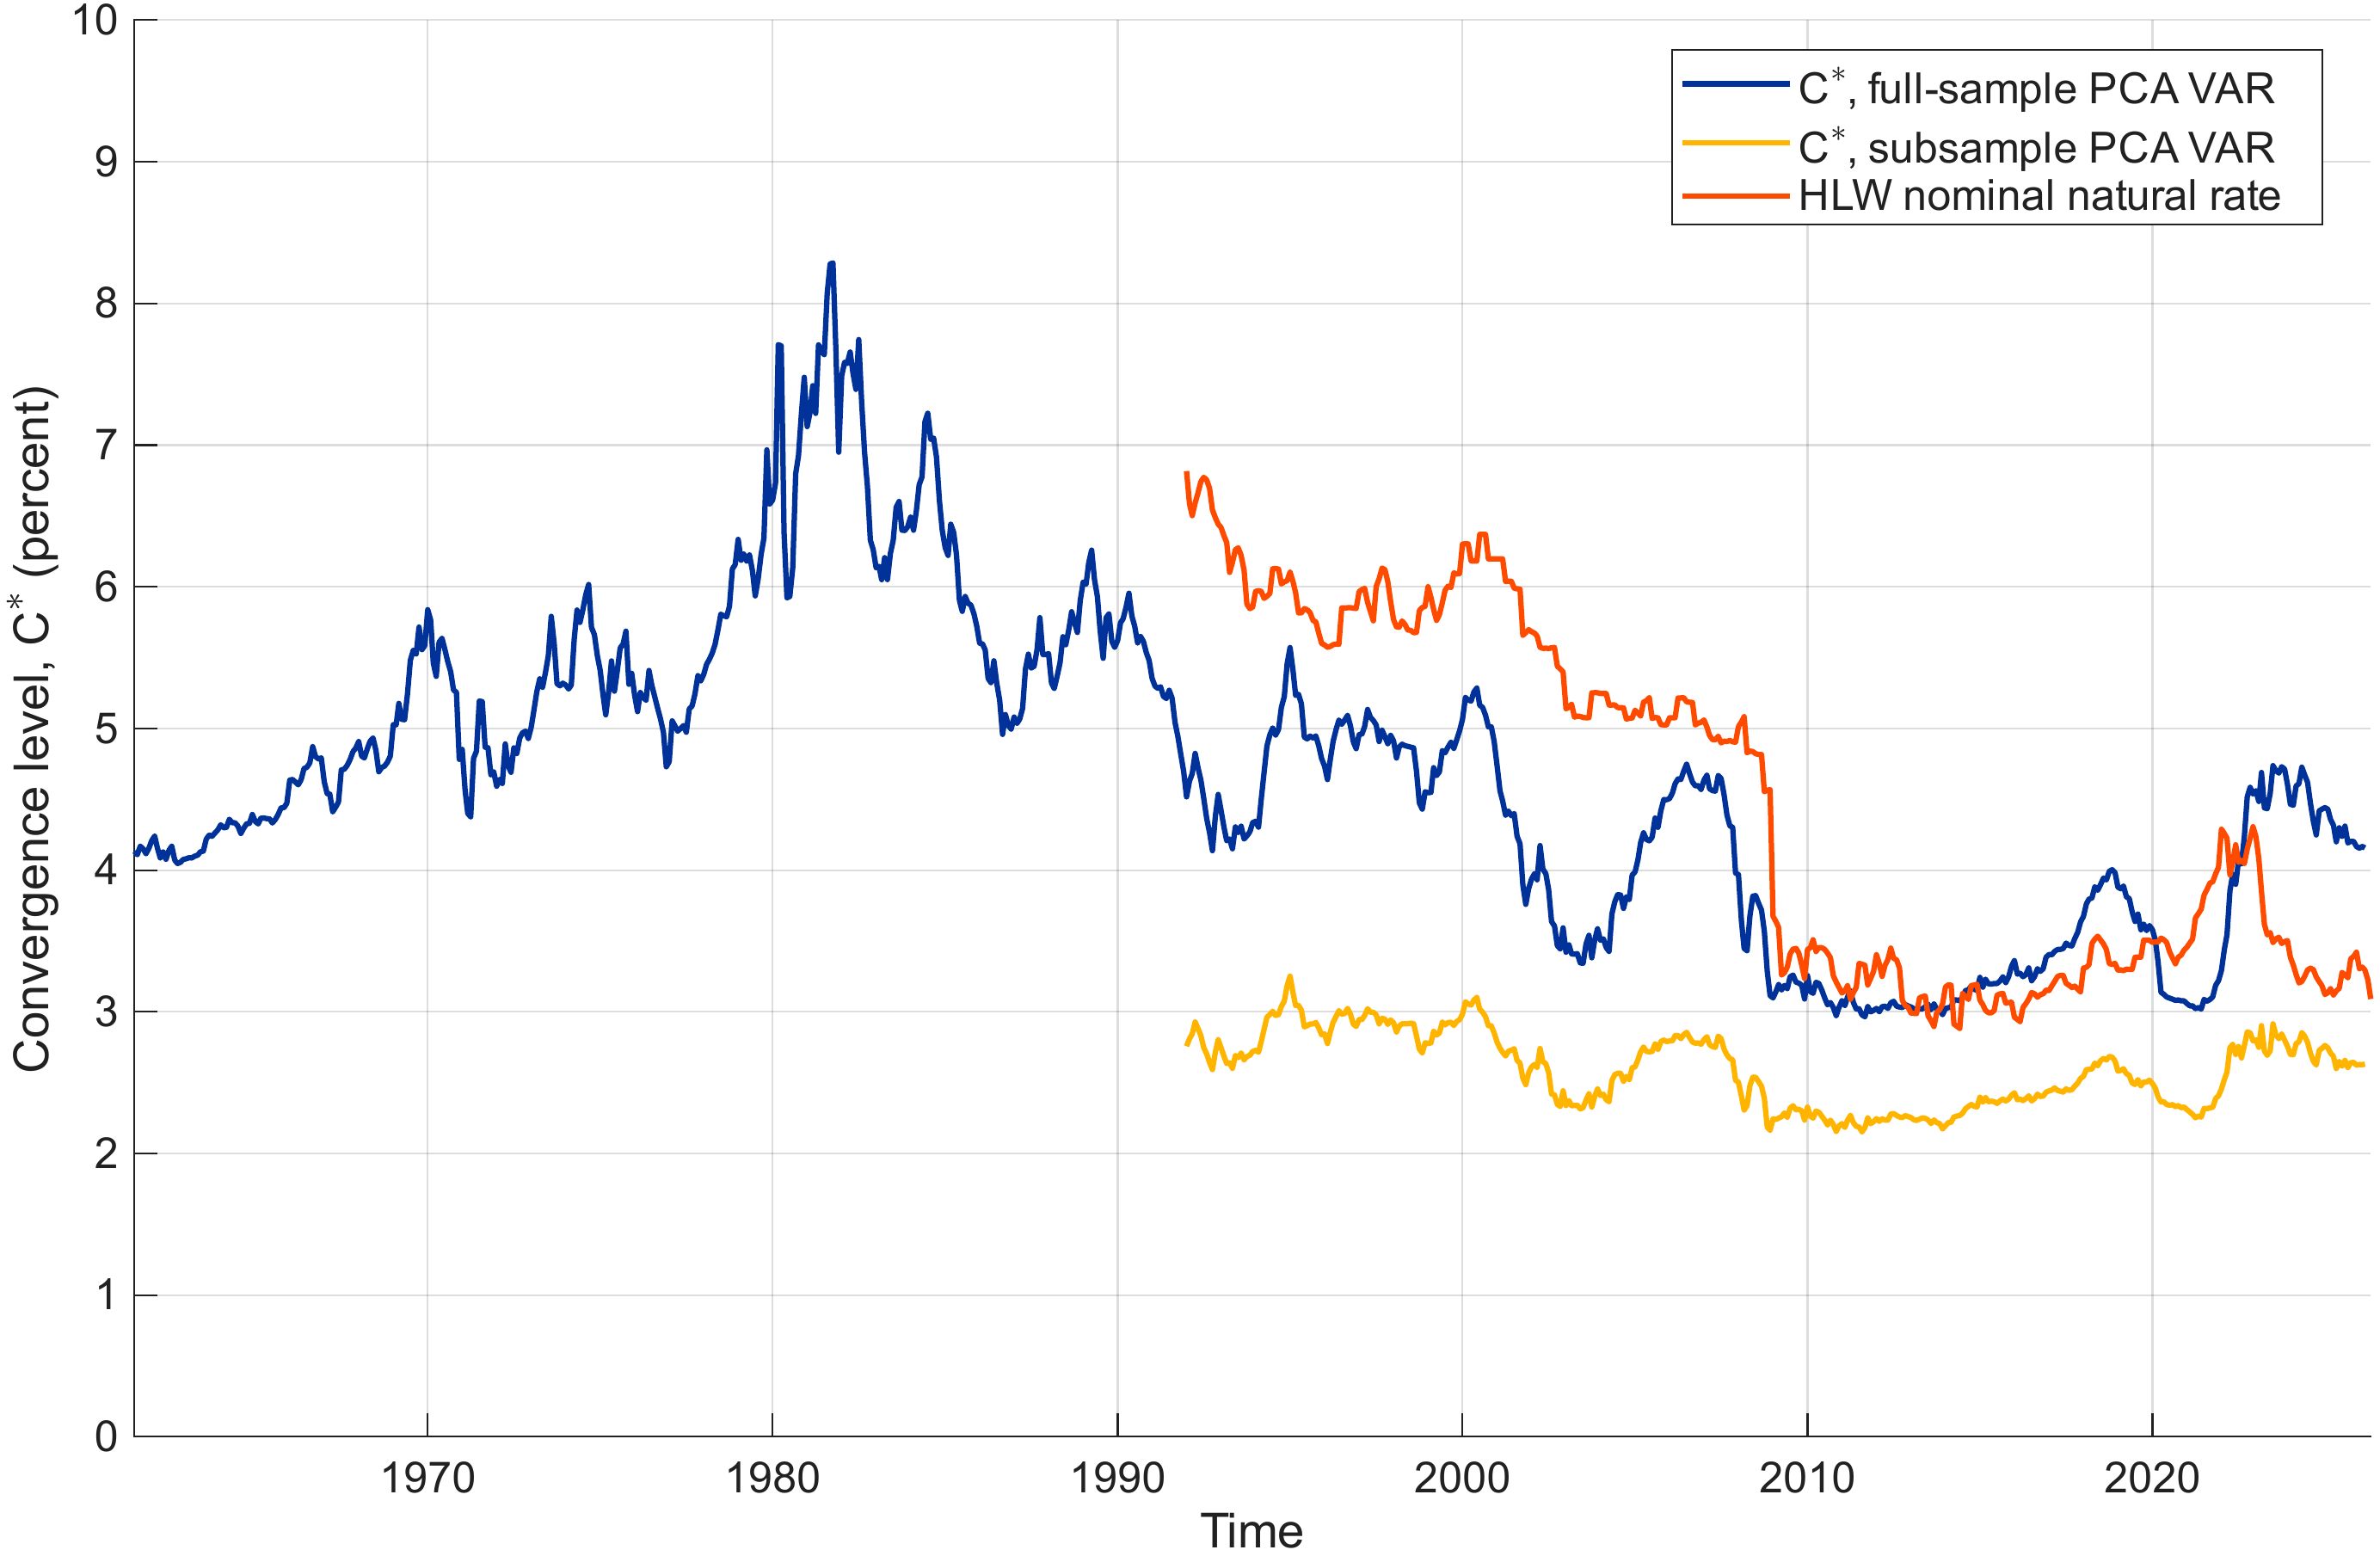
\includegraphics[width=0.8\linewidth,height=\textheight,keepaspectratio]{img/Cstar.png}

}

\caption{\label{fig-Cstar}Nominal short-rate convergence levels,
\(C^{\ast}\)}

\end{figure}%

\emph{The figure plots three alternative estimates of the nominal
short-rate convergence level, \(C^{\ast}\), in percent. The blue line
shows \(C^{\ast}\) implied by a VAR(1) estimated on the first three
principal components of Treasury yields using the full sample from 1961
to 2026. The orange line shows the corresponding \(C^{\ast}\) estimate
when the VAR is re-estimated on the subsample starting in 1991. The
yellow line shows the nominal natural rate obtained by adding 10-year
inflation expectations from the Philadelphia Fed to the real
\(r^{\ast}\) estimates of Holston et al. (2017). All series are monthly
and are plotted over the period shown on the horizontal axis.}

Figure~\ref{fig-Cstar} compares three time series for the nominal
short-rate convergence level \(C^{\ast}\), estimated over nearly six
decades of US data. The blue line shows the convergence level implied by
a VAR(1) fitted to the first three principal components of Treasury
yields over the full sample from the early 1960s to 2026. This series
displays a pronounced rise through the high-inflation 1970s, peaking in
the early 1980s, followed by a gradual secular decline that brings
\(C^{\ast}\) down to around 3--4 percent by the 2010s. The orange line
shows the corresponding VAR-based estimate when the model is
re-estimated on a shorter sample starting in 1991. While it largely
tracks the full-sample estimate over the overlapping period, it places
\(C^{\ast}\) noticeably higher during the late 1990s and early 2000s,
and somewhat higher again after the global financial crisis. This
highlights the sensitivity of the implied terminal rate to the
estimation window and, by implication, to assumptions about which
historical episodes are informative for current long-run expectations.

The yellow line shows the nominal natural rate, \(C^{\ast}\) constructed
by adding 10-year inflation expectations from the Philadelphia Fed to
the real \(r^{\ast}\) estimates of . This series is smoother and lies
below the two VAR-based estimates for most of the sample, particularly
in the 1970s and early 1980s. From the mid-1990s onwards, the HLW-based
series remains in a relatively narrow range around 2.5--3 percent,
suggesting that the long-run neutral nominal rate has been considerably
more stable than the terminal short-rate levels implied by purely
yield-based VARs. The gap between the VAR-implied \(C^{\ast}\) and the
HLW nominal natural rate therefore measures the extent to which the
yield curve embeds additional information---whether about risk premia,
perceived regime shifts, or other factors---that is not captured by
macro-based neutral-rate estimates. This comparison underscores the key
message of the Terminal Rate Model: the long-run anchor of the risk-free
term structure is both quantitatively important and model-dependent, and
alternative ways of pinning down \(C^{\ast}\) can lead to materially
different interpretations of yield curve movements and term premia.

The outcome is that that term premia estimates are significantly
different. To focus on these differences the \(2\) and \(10\) year term
premia are plotted in Figure~\ref{fig-termpremia} below.

\begin{figure}

\centering{

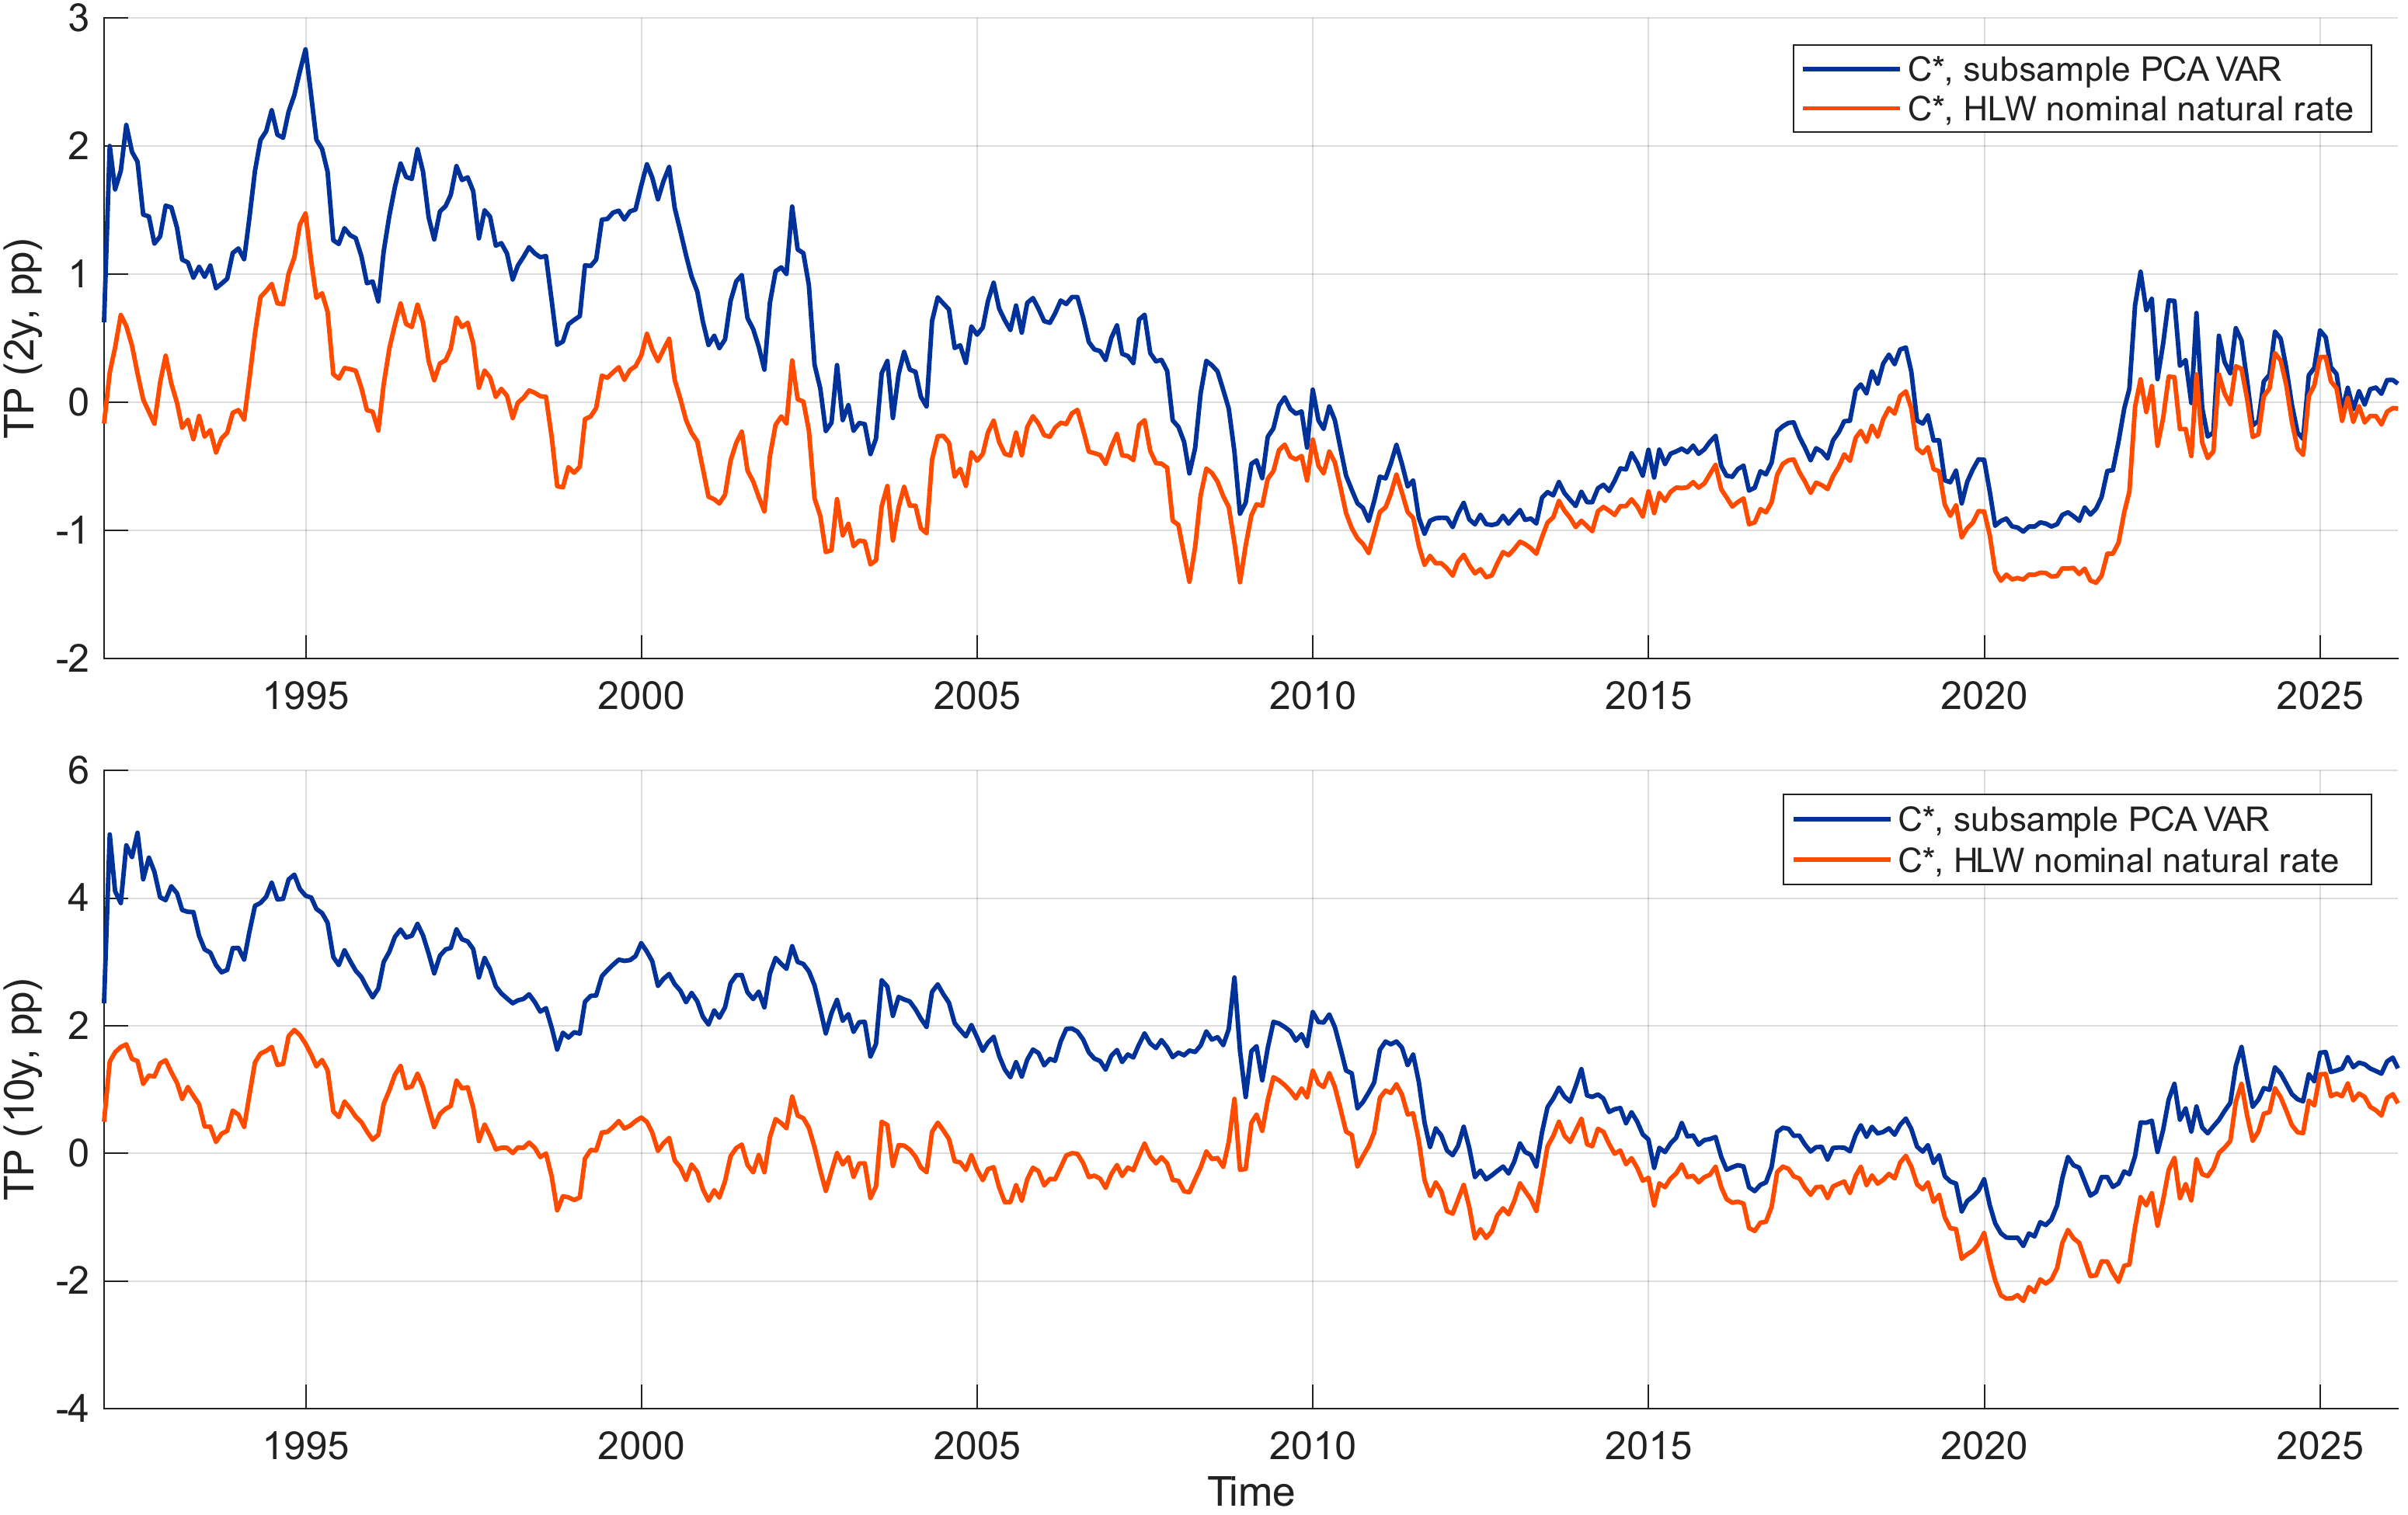
\includegraphics[width=0.8\linewidth,height=\textheight,keepaspectratio]{img/termpremia_trm_var.png}

}

\caption{\label{fig-termpremia}Term premia estimates}

\end{figure}%

\emph{The figure plots term premia at the 2-year maturity (top panel)
and the 10-year maturity (bottom panel), both in percentage points,
estimated from the Terminal Rate Model over the period 1991--2026. The
blue line corresponds to the model estimated with \(C^{\ast}\) set equal
to the subsample PCA VAR convergence level, and the orange line
corresponds to \(C^{\ast}\) set equal to the nominal natural rate of to
which \(10\)-year inflation expectations from the Philadelphia Fed's
survey of professional forecasters is added. All series are monthly.}

The consequences of the two alternative \(C^{\ast}\) specifications are
immediately apparent in Figure~\ref{fig-termpremia}, which plots the
implied term premia at the 2- and 10-year maturities. The most striking
feature of both panels is the persistent and substantial gap between the
two series throughout much of the sample. Since a higher \(C^*\) implies
that the market is compensating investors for a future short rate
converging to a higher long-run level, it compresses the term premium: a
larger share of the observed yield is attributed to rate expectations
rather than to risk compensation. Conversely, a lower \(C^{\ast}\)
leaves more of the yield to be explained by the term premium component.
This is exactly the pattern visible in the figure: in periods where the
HLW-based \(C^*\) lies below the VAR-based estimate---as it does
throughout most of the sample---the orange series registers higher term
premia than the blue.

At the 2-year horizon, the difference between the two series is already
economically meaningful, with gaps frequently exceeding 100 basis points
and, in some episodes, approaching 200 basis points. Crucially, the two
series at times assign opposite signs to the 2-year term premium: the
VAR-based estimate dips firmly into negative territory during the
post-GFC easing cycle and again in the years around 2015--2019, whereas
the HLW-based estimate remains positive or close to zero over these same
periods. The sign of the term premium has a direct bearing on how one
interprets yield curve dynamics and monetary policy transmission, so
this disagreement is not merely quantitative but qualitative.

The 10-year panel tells a broadly similar story, but with greater
absolute magnitudes and a more pronounced secular trend. Both series
decline over the sample, consistent with the well-documented compression
of long-term risk premia following the Greenspan era and during the
period of unconventional monetary policy. The VAR-based estimate falls
more steeply, reaching negative values after the GFC and remaining
subdued until the post-pandemic inflation shock of 2022--2023, when both
series surge sharply upward as the Federal Reserve tightened
aggressively. The HLW-based estimate tracks this broad narrative as well
but at a consistently higher level, suggesting that an economically
anchored \(C^{\ast}\) attributes a greater fraction of any given long
yield to a positive risk compensation, and a smaller fraction to mere
rate expectations.

Two further observations are worth highlighting. First, the co-movement
between the two series---while far from perfect---is sufficiently
positive to confirm that they are capturing the same underlying
risk-premium dynamics to a meaningful degree; the divergence is
therefore a level shift rather than noise. Second, the spread between
the two estimates narrows considerably in the post-2022 episode, when
the aggressive and broadly anticipated hiking cycle brought \(C^*\)
estimates derived from market yields and from macro fundamentals into
closer alignment. This convergence is itself informative: it suggests
that, in regimes where the market's long-run anchor is well pinned by
actual policy expectations, the identification uncertainty around
\(C^*\) diminishes, and the different specifications produce more
concordant term premium estimates.

Taken together, Figure~\ref{fig-termpremia} illustrates the central
practical message of the Terminal Rate Model: term premium estimates are
not model-free quantities, and the long-run convergence level
\(C^{\ast}\) is not a minor technical detail but a first-order
determinant of the resulting decomposition. Practitioners and
researchers who compare term premia across models or datasets must
therefore be alert to differences in the implicit or explicit
\(C^{\ast}\) assumption embedded in each.

\bookmarksetup{startatroot}

\chapter{Defined-Benefit Pensions}\label{sec:IntroPensions}

\begin{tcolorbox}[enhanced jigsaw, arc=.35mm, bottomrule=.15mm, breakable, colback=white, colframe=quarto-callout-color-frame, left=2mm, leftrule=.75mm, opacityback=0, rightrule=.15mm, toprule=.15mm]

This chapter covers the following topics:

\begin{itemize}
\tightlist
\item
  Basic principles of defined pension benefits.
\item
  Key parameters, and the pension conversion factor.
\item
  Asset and liability considerations.
\item
  Solvency calculations.
\item
  Early retirement factors.
\item
  Transfers to and from the plan.
\end{itemize}

\end{tcolorbox}

This chapter examines defined benefit pension schemes. Under such
arrangements, the pension provider promises to pay the pension recipient
an annuity that starts at a later point in time, based on terms that are
agreed upon when the agreement is made. In occupational schemes, the
provider is typically the employer and the recipient an employee,
whereas in market-based arrangements the provider is a financial
institution and the recipient a private individual.

The funding of future pension payments is achieved through regular,
typically monthly, contributions. Occasional irregular payments, known
as transfer-ins, can also be made. Pension savings often benefit from a
favourable tax treatment. In occupational schemes, contributions are
usually deducted from the pre-tax salary, which lowers the employee's
taxable income and thus the size of the immediate tax bill. Moreover,
returns generated from the invested funds are exempt from taxation
during the accumulation phase. Tax is only payable once the annuity
payments start, allowing the funds to compound more rapidly on a larger
base. At retirement, the recipient is typically in a lower tax bracket
than during active employment, which further reduces the overall tax
bill across the person's lifetime.

Pension analysis integrates long-term investment management, the
transfer of risk between the employee (the pension recipient) and the
plan sponsor (the pension provider), asset--liability matching, and
comprehensive risk monitoring. It is therefore a discipline that unites
several key elements of financial theory and analytical practice.

While the discussion is general, for ease of notation and narrative
clarity, I will refer to the pension provider as the `plan sponsor' and
the pension recipient as the `employee'. This terminology aligns with
occupational pension schemes but is adopted here purely for convenience.

Defined-benefit (DB) pension plans promise employees a pre-specified
stream of retirement income that is linked to salary and service, rather
than to the realised performance of the underlying investments.
Figure~\ref{fig-pensionOverview} illustrates the phases of pension cash
flows for a single employee over the full life cycle of a DB
arrangement. At time \(t_0\) the employee joins the pension scheme and
starts making contributions toward the funding of the pension;
typically, the employer also contributes a fixed fraction of the
employee's salary, as specified in the employment contract.

\begin{figure}

\centering{

\pandocbounded{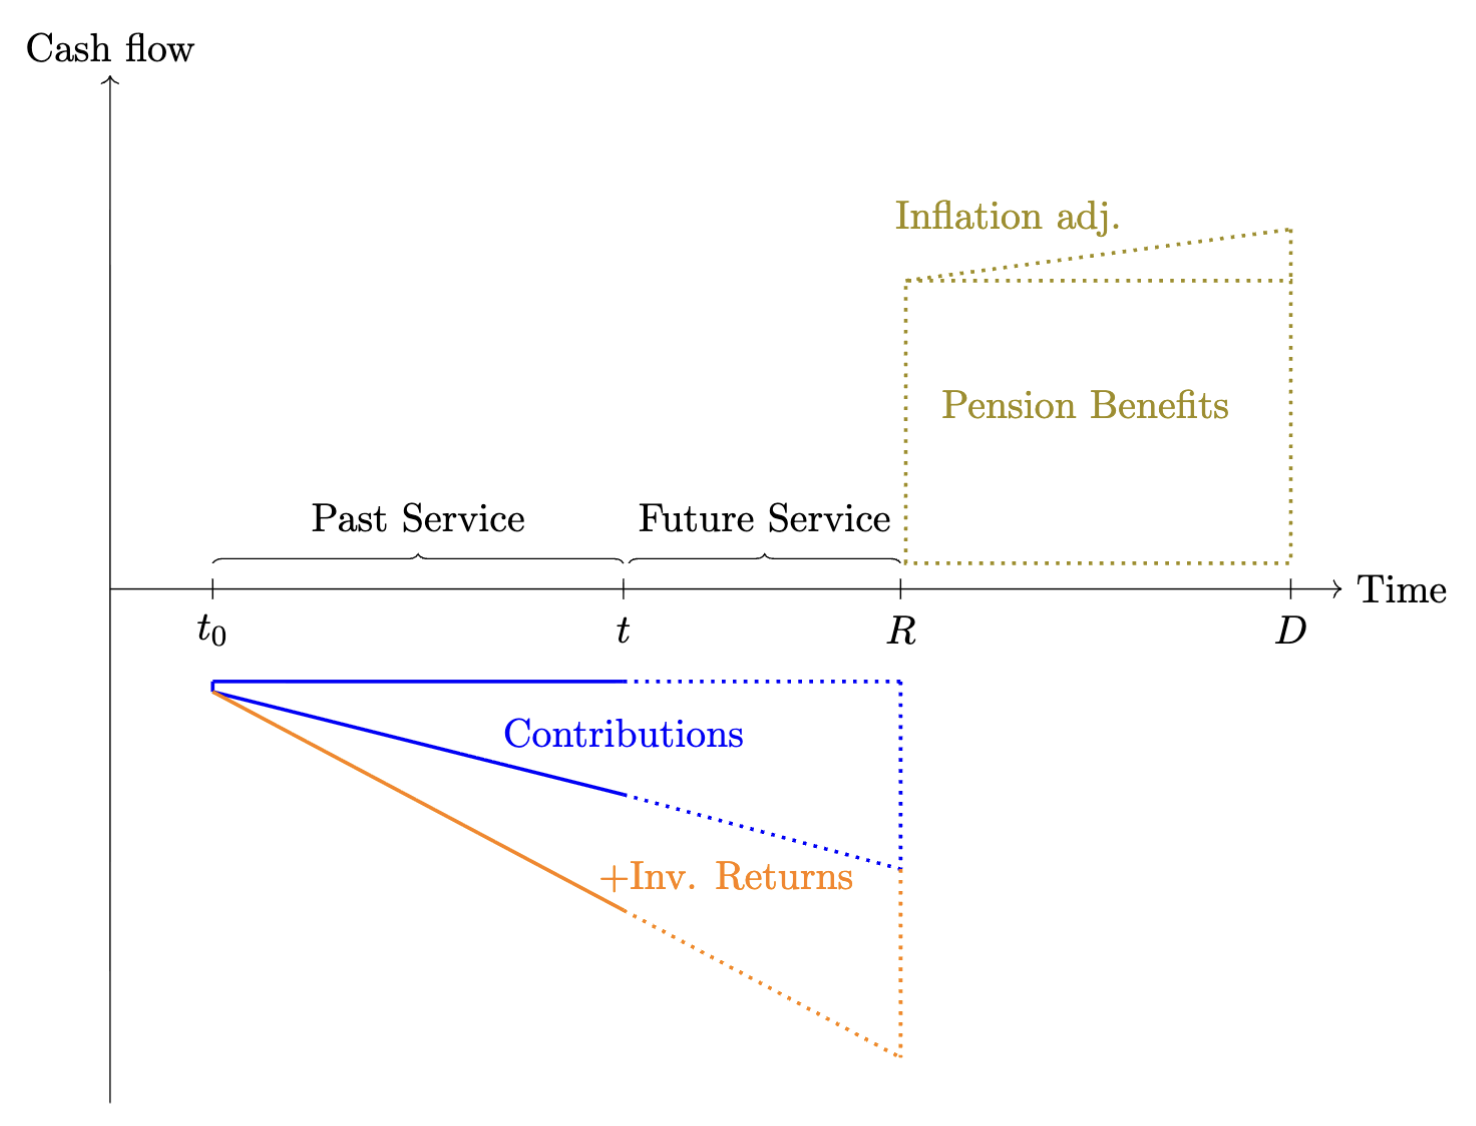
\includegraphics[keepaspectratio]{img/DBPension_fig_overview.png}}

}

\caption{\label{fig-pensionOverview}Pension cash flows}

\end{figure}%

Between \(t_0\) and the retirement date \(R\) the member accumulates
service years in the pension plan. Figure~\ref{fig-pensionOverview}
distinguishes between past service, from \(t_0\) up to the date \(t\)
where it is assumed that the funding level of the plan is assessed
(e.g.~through an actuarial funding study or an assessment made by the
employer), and future service, from \(t\) to retirement at \(R\). The
solid blue and orange lines illustrate the build-up of pension assets
due to contributions and investment returns; the dotted extensions
indicate the continuation of these flows over the future-service period.
At the retirement date \(R\), the DB pension is paid out as an annuity
that grows according to the agreed pension indexation until the time of
death \(D\). Geometrically, a pension plan is well funded when the area
of the combined triangle formed by contributions and investment returns
matches the area of the rectangle representing the pension annuity
together with the triangular area capturing the annuity's indexation
over time.

In a stylised but widely used formulation, the annual pension benefit at
retirement is given by
\begin{equation}\protect\phantomsection\label{eq-pb_def}{
    PB = \alpha \cdot SY \cdot FS,
}\end{equation} where \(PB\) denotes the annual pension benefit,
\(\alpha\) is the accrual rate per year of service (for example
\(2\%\)), \(SY\) is the number of service years accumulated in the plan,
and \(FS\) is the final salary at retirement. This simple benefit
formula links the length of the past-service period and the level of
final pay to the height of the pension-benefit rectangle in
Figure~\ref{fig-pensionOverview} . It also highlights the defining
feature of DB schemes: pension payments are contractually guaranteed by
the sponsor, and the financial and demographic risks required to honour
Equation~\ref{eq-pb_def} are borne by the plan sponsor (employer) rather
than by the individual member.

\section{Funding ratio and basic
valuation}\label{funding-ratio-and-basic-valuation}

From a valuation perspective, the central task at time \(t\) is to
compare (i) the present value of all past-service contributions and
accumulated investment returns to date, represented by the blue and
orange areas to the left of \(t\) in Figure~\ref{fig-pensionOverview},
with (ii) the present value of the accrued portion of the
pension-benefit rectangle to the right of \(R\). Denote by \(A_t\) the
market value of the pension assets at time \(t\) and by \(L_t\) the
actuarial present value of accrued pension liabilities at the same date.
The funding ratio at time \(t\) is defined as
\begin{equation}\protect\phantomsection\label{eq-FR_def}{
    FR_t = \frac{A_t}{L_t},
}\end{equation} which is the standard summary indicator of the solvency
position of DB arrangements. Values of \(FR_t\) below one indicate
underfunding (assets are insufficient to cover the present value of
accrued benefits), whereas values above one indicate a funding surplus.
In equilibrium, the discounted area under the contribution and return
profiles matches the discounted area of the pension-benefit block plus
the inflation adjustments.

\section{Deterministic retirement
horizon}\label{deterministic-retirement-horizon}

Figure~\ref{fig-pensionOverview} labels \(D\) as the expected date of
death. In a basic version of the framework, one treats \(R\) and \(D\)
as fixed, so that the member is assumed to receive benefits over a
deterministic retirement horizon of length \[
    t_{DR} = D - R.
\] The pension-benefit rectangle between \(R\) and \(D\) in the figure
is then interpreted literally: \(PB\) (indexed to inflation) is paid
every year from \(R\) until \(D\), and no benefits are paid outside this
interval.

Let \(r_d\) denote the nominal discount rate and \(r_{inf}\) the annual
rate at which pension benefits are indexed (for example the inflation
rate). The annual pension at retirement is \(PB\), and it grows at the
rate \(r_{inf}\) each year between \(R\) and \(D\). Under these
assumptions, the present value of the pension benefits at the retirement
date \(R\) can be expressed as the present value of a finite,
inflation-indexed annuity:
\begin{equation}\protect\phantomsection\label{eq-PV-R-deterministic}{
PV_{R}(PB) = PB \cdot \frac{1}{r_d - r_{inf}} \left[ 1 - \left(\frac{1 + r_{inf}}{1 + r_d}\right)^{t_{DR}} \right].
}\end{equation} If \(t\) denotes the valuation date and \(t_R = R - t\)
the number of years from \(t\) to retirement, the present value of the
liabilities at the valuation date is obtained by discounting
Equation~\ref{eq-PV-R-deterministic} back \(t_R\) years:
\begin{equation}\protect\phantomsection\label{eq-PV-t-deterministic}{
    L_{t} \;=\; PV_{t}(PB) = PV_R(PB) \cdot (1 + r_d)^{-t_R}.
}\end{equation}

Substituting Equation~\ref{eq-PV-t-deterministic} into
Equation~\ref{eq-FR_def} yields a closed-form expression for the funding
ratio when both the retirement date and the date of death are assumed
deterministic. In terms of Figure~\ref{fig-pensionOverview}, the
deterministic-horizon valuation discounts the entire green benefit
rectangle back to the valuation date \(t\) using a fixed horizon of
length \(t_R + t_{DR}\).

\section{Generalising to survival
probabilities}\label{generalising-to-survival-probabilities}

In practice, the date of death \(D\) in Figure~\ref{fig-pensionOverview}
is uncertain: the height the pension-benefit block is known, but the
right-hand edge, and thus the width, is random. For actuarial work it is
therefore conceptually cleaner, to treat the retirement horizon as
random by modelling mortality explicitly. For this, we apply the
following notation and work in annual steps (a generalisation to monthly
or daily steps is straight forward):

\begin{itemize}
\tightlist
\item
  \({}_tp_y\) is the probability that a person aged \(y\) survives at
  least \(t\) more years.
\item
  \(v = (1 + r_d)^{-1}\) is the annual discount factor.
\end{itemize}

Assume that the pension commences at age \(y\) with an initial annual
amount of \(PB\) that is indexed annually at the rate of \(r_{inf}\).
The payment at age \(y + k\) is then \[
    \text{Benefit at age}\; y + k = PB \cdot (1 + r_{inf})^{k}, \qquad k = 0,1,2,\dots.
\] In the diagram, these payments correspond to vertical slices of the
pension-benefit rectangle at successive points in time. The probability
that the member is alive to receive the payment at age \(y + k\) is
\({}_k p_y\), and the payment is discounted back to the valuation age,
denoted by \(x\), using \(v^{(y - x)+k}\). The actuarial present value
at age \(x\) of the pension benefits is therefore
\begin{equation}\protect\phantomsection\label{eq-PV_x_general}{
    L_t \;\equiv\; PV_x(PB) = v^{\,y - x} \sum_{k=0}^{\infty} PB \cdot (1 + r_{inf})^{k} \cdot v^{k} \cdot {}_k p_r.
}\end{equation} \(PB\) can be factored out, and the inner sum is
therefore a growing life annuity starting at age \(y\): \[
    PV_x(PB) = PB \cdot v^{\,y - x} \cdot \ddot{a}^{g}_y,
\] where \[
    \ddot{a}^{g}_y = \sum_{k=0}^{\infty} (1 + r_{inf})^{k} v^{k} \, {}_k p_y
\] is the expected present value, at age \(y\), of a payment of one unit
per year, increasing at rate \(r_{inf}\), payable while the member is
alive.

Substituting Equation~\ref{eq-PV_x_general} into
Equation~\ref{eq-FR_def} gives the funding ratio in the general
mortality framework:
\begin{equation}\protect\phantomsection\label{eq-FR_general}{
    FR_t = \frac{A_t}{PV_x(PB)} \;=\; \frac{A_t}{v^{\,y - x} \displaystyle \sum_{k=0}^{\infty} PB \cdot (1 + r_{inf})^{k} \cdot v^{k} \cdot {}_k p_y }.
}\end{equation} Relative to the deterministic-horizon case, the
right-hand boundary of the benefit block in
Figure~\ref{fig-pensionOverview} is now stochastic: each potential
payment year contributes to \(L_t\) with a weight equal to the
probability that the member is still alive at that age.

\section{The deterministic horizon as a special
case}\label{the-deterministic-horizon-as-a-special-case}

The deterministic-lifespan assumption used in
\textbf{?@eq-PV\_R\_deterministic} -- \textbf{?@eq-PV\_t\_deterministic}
emerges as a special case of the more general survival-probability
framework. Suppose that the member is assumed to be certain to survive
from retirement until a fixed age \(D\) and to die with certainty at
that age. In actuarial terms this corresponds to
\begin{equation}\protect\phantomsection\label{eq-survival}{
\begin{aligned}
    {}_k p_y &= 1, \qquad k = 0,1,\dots,t_{DR}-1, \\
    {}_k p_y &= 0, \qquad k \ge t_{DR}
\end{aligned}
}\end{equation} where \(t_{DR} = D - y\) is now a deterministic
retirement horizon. Substituting these survival probabilities into
Equation~\ref{eq-PV_x_general} gives \[
    PV_x(PB) = v^{\,y - x} \sum_{k=0}^{t_{DR}-1} PB \cdot (1 + r_{inf})^{k} \cdot v^{k},
\] which is exactly the present value of a finite growing annuity with
\(t_{DR}\) payments, indexed at rate \(r_{inf}\) and discounted at rate
\(r_d\). Evaluating the finite sum yields \[
    PV_x(PB) = v^{\,y - x} \cdot PB \cdot \frac{1}{r_d - r_{inf}} \left[1 - \left(\frac{1 + r_{inf}}{1 + r_d}\right)^{t_{DR}} \right],
\] which coincides with \textbf{?@eq-PV\_R\_deterministic} --
\textbf{?@eq-PV\_t\_deterministic} when \(x\) is interpreted as the
valuation age and \(y - x = t_R\). Thus, the closed-form valuation of
liabilities under a fixed lifespan can be seen as the special case of a
general mortality model in which the retirement horizon is degenerate
rather than stochastic. In the same way, the general funding-ratio
formula Equation~\ref{eq-FR_general} reduces to the
deterministic-horizon expression obtained by inserting
\textbf{?@eq-PV\_t\_deterministic} into Equation~\ref{eq-FR_def}.

\section{A simple numerical
illustration}\label{a-simple-numerical-illustration}

To connect the geometry of Figure~\ref{fig-pensionOverview} with actual
magnitudes, consider a worker aged \(x = 45\) who retires at age
\(y = 65\) with an annual pension benefit determined by
Equation~\ref{eq-pb_def}. Suppose the final salary at retirement is
\(FS = 65{.}000\), the accrual rate is \(\alpha = 2\%\), and the worker
has \(SY = 35\) service years at retirement. Then the height of the
pension-benefit rectangle at retirement is \[
    PB = 0.02 \cdot 35 \cdot 65{.}000 \;=\; 45{.}500.
\] Assume a nominal discount rate of \(r_d = 3\%\) and an indexation
rate of \(r_{inf} = 2\%\), so \(v = (1.03)^{-1}\).

\subsubsection{Deterministic horizon.}\label{deterministic-horizon.}

If we first assume a deterministic retirement horizon of \(t_{DR} = 20\)
years (for example from age 65 to 85), the present value of pension
benefits at retirement is \[
    PV_{R}(PB) = 45{.}500 \cdot \frac{1}{0.03 - 0.02} \left[ 1 - \left(\frac{1.02}{1.03}\right)^{20} \right],
\] and the present value at age \(45\) is
\(PV_{45}(PB) = PV_R(PB) \cdot (1.03)^{-20}\). If the asset value at age
\(45\) is \(A_{45}\), the corresponding funding ratio under this
deterministic horizon is \(FR_{45} = A_{45} / PV_{45}(PB)\).

\subsubsection{Stochastic horizon with survival
probabilities.}\label{stochastic-horizon-with-survival-probabilities.}

Now replace the deterministic horizon with survival probabilities drawn
from an appropriate life table. Let \({}_k p_{65}\) denote the
probability that a person aged \(65\) today survives at least \(k\) more
years. The present value at age \(45\) becomes \[
    PV_{45}(PB)  = v^{20} \sum_{k=0}^{\infty} 45{.}500 \cdot (1.02)^{k} \cdot v^{k} \cdot {}_kp_{65},
\] and the corresponding funding ratio is \[
    FR_{45} = \frac{A_{45}}{PV_{45}(PB)}.
\] For typical mortality patterns, the sum is effectively truncated at
ages where \({}_k p_{65}\) becomes negligible. Relative to the
deterministic case with the same maximum age, incorporating realistic
survival probabilities generally reduces the liability value because
some members die earlier and therefore receive fewer payments in
expectation. In terms of Figure~\ref{fig-pensionOverview}, the right
edge of the benefit block is now random rather than fixed, and the
expected height--width area of the green rectangle shrinks once survival
probabilities are taken into account.

\section{Early retirement penalty factors}\label{sec:penaltyFactors}

In many occupational pension schemes, the retirement date is to some
extent discretionary, allowing employees to retire earlier than the
scheme's standard retirement age. Choosing early retirement brings the
start of the pension annuity forward, so payments are made over a longer
period. At the same time, fewer service years have been accrued, so the
benefit formula delivers a lower annual pension.

For example, if the normal retirement age is 65, employees may be
permitted to retire as early as age 55. In such cases, pension benefits
are typically reduced by a penalty factor---a percentage deduction
applied for each year of early retirement. Under an actuarially neutral
approach, the penalty is calibrated such that the present value of the
early retirement pension equals the present value of the income stream
beginning at the normal retirement age. With \(R\) denoting the normal
retirement age, and \(E<R\) be an admissible early retirement age, the
requirement for actuarial neutrality is that
\begin{equation}\protect\phantomsection\label{eq-actuarialNeutralEarlyRetirement}{
    PV_E(PB_E) = PV_E(PB_R).
}\end{equation} Using equation Equation~\ref{eq-pb_def} early retirement
benefits are given by: \[
   PV_E(PB_E) = \alpha \cdot SY_E \cdot FS \cdot (1+\mathbb{E}\left[r_{sgr}\right])^{E-R},
\] where \(r_{sgr}\) is the annual salary growth rate, assumed to be
constant across years. At the same time, the present value of the of the
pension benefit at normal retirement, at early retirement, is: \[
    PV_E(PB_R) = \alpha \cdot SY_R \cdot FS \cdot v^{R-E} \cdot {}_{(R-E)}p_E.
\] Using Equation~\ref{eq-actuarialNeutralEarlyRetirement}, and defining
\(v_{sgr}=(1+\mathbb{E}\left[r_{sgr}\right])^{-1}\) the actuarial
neutral early retirement penalty factor can be expressed as: \[
\begin{aligned}
    P_{E\leftarrow R} &= \frac{\alpha \cdot SY_E \cdot FS \cdot v_{sgr}^{R-E}}{\alpha \cdot SY_R \cdot FS \cdot v^{R-E} \cdot {}_{(R-E)}p_E} \nonumber \\ 
    &= \frac{ SY_E \cdot v_{sgr}^{R-E}}{SY_R \cdot v^{R-E} \cdot {}_{(R-E)}p_E} \nonumber \\
    &= \frac{SY_E}{SY_R \cdot {}_{(R-E)}p_E} \left( \frac{v_{sgr}}{v} \right)^{R-E}
\end{aligned}
\] This expression highlights three distinct components. First, the
ratio \(\frac{SY_E}{SY_R}\) captures the effect of shorter service at
the early retirement age: with fewer accrual years, the pensionable
salary at age \(E\) is typically lower than at age \(R\). Second, the
term \({}_{(R-E)}p_E\) in the denominator reflects survival over the
period from \(E\) to \(R\), so that a lower probability of reaching the
normal retirement age implies a higher actuarial penalty for bringing
payments forward. Finally, the factor
\(\left(\frac{v_{sgr}}{v}\right)^{R-E}\) isolates the interaction
between expected salary growth and financial discounting over the
interval \([E,R]\): if expected salary growth (embedded in \(v_{sgr}\))
offsets part of the pure financial discounting (captured by \(v\)), the
overall penalty is reduced, whereas if discounting dominates expected
salary growth the penalty becomes more severe.

Table~\ref{tbl-penaltyFactors} reports example calculations for the
actuarially neutral early retirement penalty factors for retirement ages
\(t=55,\ldots,65\), relative to the normal retirement age 65. The salary
growth rate is assumed to be \(r_{\text{sgr}} = 2.4\%\) per year, while
the discount rate is \(r_{d} = 3\%\) per year. The survival
probabilities \({}_{(65-t)}p_{t}\) are based on the ICSLT 2023 mortality
table and reflect the average of male and female survival probabilities.
The column labelled \(SY_{E}/SY_{R}\) captures the ratio of service
years at the early and normal retirement ages relative to the normal
retirement age of 65 years. \((v_{\text{sgr}}/v)^{65-t}\) reflects the
interaction between the salary growth rate and the discounting rate. The
final two columns show the resulting penalty factor as a ratio and a
percentage reduction relative to the unreduced pension at age \(65\).

\begin{longtable}[]{@{}
  >{\raggedright\arraybackslash}p{(\linewidth - 10\tabcolsep) * \real{0.1304}}
  >{\raggedleft\arraybackslash}p{(\linewidth - 10\tabcolsep) * \real{0.1739}}
  >{\raggedleft\arraybackslash}p{(\linewidth - 10\tabcolsep) * \real{0.1739}}
  >{\raggedleft\arraybackslash}p{(\linewidth - 10\tabcolsep) * \real{0.1739}}
  >{\raggedleft\arraybackslash}p{(\linewidth - 10\tabcolsep) * \real{0.1739}}
  >{\raggedleft\arraybackslash}p{(\linewidth - 10\tabcolsep) * \real{0.1739}}@{}}
\caption{Actuarially neutral early retirement penalty
factors}\label{tbl-penaltyFactors}\tabularnewline
\toprule\noalign{}
\begin{minipage}[b]{\linewidth}\raggedright
\(t\)
\end{minipage} & \begin{minipage}[b]{\linewidth}\raggedleft
\({}_{(65-t)}p_t\)
\end{minipage} & \begin{minipage}[b]{\linewidth}\raggedleft
\(SY_E/SY_R\)
\end{minipage} & \begin{minipage}[b]{\linewidth}\raggedleft
\((v_{\text{sgr}}/v)^{65-t}\)
\end{minipage} & \begin{minipage}[b]{\linewidth}\raggedleft
Penalty ratio
\end{minipage} & \begin{minipage}[b]{\linewidth}\raggedleft
Penalty (\%)
\end{minipage} \\
\midrule\noalign{}
\endfirsthead
\toprule\noalign{}
\begin{minipage}[b]{\linewidth}\raggedright
\(t\)
\end{minipage} & \begin{minipage}[b]{\linewidth}\raggedleft
\({}_{(65-t)}p_t\)
\end{minipage} & \begin{minipage}[b]{\linewidth}\raggedleft
\(SY_E/SY_R\)
\end{minipage} & \begin{minipage}[b]{\linewidth}\raggedleft
\((v_{\text{sgr}}/v)^{65-t}\)
\end{minipage} & \begin{minipage}[b]{\linewidth}\raggedleft
Penalty ratio
\end{minipage} & \begin{minipage}[b]{\linewidth}\raggedleft
Penalty (\%)
\end{minipage} \\
\midrule\noalign{}
\endhead
\bottomrule\noalign{}
\endlastfoot
55 & 0.97639 & 0.71429 & 1.06016 & 0.78 & 22\% \\
56 & 0.97772 & 0.74286 & 1.05399 & 0.80 & 20\% \\
57 & 0.97921 & 0.77143 & 1.04785 & 0.83 & 17\% \\
58 & 0.98087 & 0.80000 & 1.04174 & 0.85 & 15\% \\
59 & 0.98273 & 0.82857 & 1.03568 & 0.87 & 13\% \\
60 & 0.98482 & 0.85714 & 1.02964 & 0.90 & 10\% \\
61 & 0.98716 & 0.88571 & 1.02364 & 0.92 & 8\% \\
62 & 0.98981 & 0.91429 & 1.01768 & 0.94 & 6\% \\
63 & 0.99280 & 0.94286 & 1.01175 & 0.96 & 4\% \\
64 & 0.99617 & 0.97143 & 1.00586 & 0.98 & 2\% \\
65 & 0.99617 & 1.00000 & 1.00000 & 1.00 & 0\% \\
\end{longtable}

\section{Transfers to and from the pension scheme}\label{sec:transfers}

During the savings phase of an occupational pension plan, employees may
have the possibility to transfer additional funds into the plan in order
to purchase extra pension service years. Likewise, if an employee
changes employer, it may be possible to transfer accumulated funds from
one occupational pension plan to another. In defined benefit pension
plans there is no direct link, at the individual level, between the
amounts contributed (and their investment returns) and the benefit
entitlement. Instead, employees accrue pension service years and the
pension benefits are determined by a formula, see equation
Equation~\ref{eq-pb_def}. It is therefore necessary to establish a
consistent mapping between pension service years and monetary amounts
when dealing with transfers into and out of a defined benefit
occupational pension plan.

The situation is not entirely straightforward. When funds are
transferred into a plan and converted into additional pension service
years, the plan sponsor effectively takes over the investment risk and
guarantees a future pension stream, thereby also committing to at least
a minimum investment return over (potentially) many years. Likewise,
when an employee leaves the plan, the accrued pension service years are
converted into a cash amount at the time of exit (to be transferred to
another occupational scheme) using assumptions about future investment
returns and discount rates. In both directions, typically the principle
of actuarial neutrality is imposed such that the value of the expected
promised pension benefits is consistent with the value of the underlying
funds.

To calculate actuarially neutral transfer amounts, both in and out of
the plan, a pension conversion factor, \(K_x\) at age \(x\), is used. In
its simplest form, \(K_x\) links a monetary amount \(C_x\) to an
increment in pension benefit (or, equivalently, in pension service
years) through a relation of the form \[
    \Delta PB_x = K_x \, C_x.
\] The factor \(K_x\) is chosen such that the present value of the
additional pension benefit \(\Delta PB_x\) equals the value of the
contribution \(C_x\), under the plan's economic and demographic
assumptions. Writing \(a_x\) for the present value at age \(x\) of a
life annuity of \(1\) per year, actuarial neutrality requires \[
    C_x = \Delta PB_x \, \ddot{a}_x,
\]

so that \[
    K_x = \frac{1}{\ddot{a}_x}.
\]

\section{The pension conversion factor}\label{subsec:conversionFactor}

During the savings phase, employees may transfer additional funds into
the pension plan or have capital amounts transferred from other
occupational schemes, in order to purchase extra pension service years
or to enhance their future pension benefit. Conversely, when employees
leave the plan, accrued benefits are often commuted to a capital sum and
transferred out to another scheme. In both directions, it is common
actuarial practice to impose actuarial neutrality such that the present
value of the future pension benefit must equal the monetary value of the
underlying funds.

To calculate actuarially neutral transfer amounts, a pension conversion
factor, \(K_x\) at age \(x\), is used. In its simplest form, \(K_x\)
links a monetary amount \(C_x\) at age \(x\) to an increment in the
annual pension benefit \(\Delta PB_R\) at normal retirement age \(R\):
\[
    \Delta PB_R = K_x \cdot C_x.
\] Intuitively, \(K_x\) is the price at time \(x\) of one unit of
additional annual pension at time \(R\), expressed per unit of capital
contributed at time \(x\). It reflects the time value of money, expected
investment returns on the underlying assets, and survival probabilities
between \(x\) and retirement, as well as the conversion of accumulated
wealth at \(R\) into an annuity.

To formalise this intuition, let \(\tilde{v}\) be a generic discount
factor. For any future random cash flow \(X_T\) payable at time \(T\),
the time--\(x\) value of \(X_T\) can then be written generically as \[
    PV_x(X_T) = \mathbb{E}_x\!\left[ \tilde{v}^{\,T-x} \, X_T \right],
\] In this representation, \(v_z\) plays the role of the appropriate
one--period pricing operator that embeds both financial and demographic
effects.

Now let \(K_R\) denote the pension conversion factor at the normal
retirement age \(R\). If \(C_R\) denotes the amount of capital at time
\(R\) attributable to a contribution \(C_x\) made at time \(x\), we can
write \[
    \Delta PB_R = K_R \cdot C_R.
\] From the perspective of time \(x\), the capital \(C_R\) is itself a
random variable driven by investment returns, mortality and possibly
other plan--specific features. Using the generic discount factor
\(v_z\), we have:
\begin{equation}\protect\phantomsection\label{eq-Kx_as_discounted_KR}{
    K_x \cdot C_x = \mathbb{E}_x\!\left[ K_R \, C_R \right] = v_z^{\,R-x} \cdot K_R \cdot C_x,
}\end{equation} where \(\tilde{v}\) accounts for the expected growth of
the capital \(C_x\) to \(C_R\) and discounting of \(K_R\) to time-\(x\).
Equation Equation~\ref{eq-Kx_as_discounted_KR} states that the pension
conversion factor at age \(x\) is the time--\(x\) expectation of the
at--retirement conversion factor \(K_R\), discounted back from \(R\) to
\(x\) using the appropriate pricing operator \(\tilde{v}\): \[
    K_x = \tilde{v}^{\,R-x} \cdot K_R.
\]

\subsection*{Actuarial neutrality and the annuity
value}\label{actuarial-neutrality-and-the-annuity-value}
\addcontentsline{toc}{subsection}{Actuarial neutrality and the annuity
value}

Assume that the additional pension benefit \(\Delta PB_R\) is first
payable at age \(R\) and continues as long as the member is alive, and
is indexed at rate \(r_{inf}\) per year. Recall that
\(v = (1 + r_d)^{-1}\) is the nominal discount factor used for valuing
pension liabilities. As in Section~\hyperref[sec:IntroPensions]{1}, let
\({}_t p_z\) be the probability that a person aged \(z\) today survives
at least \(t\) more years. Under these assumptions, the additional
pension stream acquired by paying \(C_x\) at age \(x\) can be described
as follows:

\begin{itemize}
\item
  At age \(R\) the member receives an additional annual pension of
  \(\Delta PB_R\).
\item
  At age \(R + k\), for \(k = 1, 2, \dots\), this additional pension is
  indexed at rate \(r_{inf}\), so the payment becomes \[
    \Delta PB_{R, R+k} = \Delta PB_R \, (1 + r_{inf})^{k}.
  \]
\item
  The probability that the member is alive at age \(R + k\) is
  \({}_k p_R\).
\item
  Payments are discounted back to age \(x\) using the factor
  \(v^{(R-x) + k}\).
\end{itemize}

The actuarial present value at age \(x\) of an additional pension of one
unit per year, starting at age \(R\) and indexed at rate \(r_{inf}\)
while the member is alive, is therefore determined by the growing life
annuity factor
\begin{equation}\protect\phantomsection\label{eq-growingLifeAnnuity}{
    \ddot{a}_x^{g} = v^{\,R - x} \sum_{k=0}^{\infty} (1 + r_{inf})^{k} \, v^{k} \, {}_k p_R
}\end{equation}

This expression is directly analogous to the general present‑value
formula Equation~\ref{eq-PV_x_general}, but specialised to an annuity of
one unit per year and with \(x\) as valuation age and \(R\) as
retirement age.

If the member receives an additional pension \(\Delta PB_x\) rather than
one unit, the present value at age \(x\) is simply \[
    PV_x(\Delta PB_x) = \Delta PB_x \, \ddot{a}_x^{g}.
\] Actuarial neutrality now requires that this present value equals the
contribution paid at age \(x\): \[
    C_x = PV_x(\Delta PB_x) \;=\; \Delta PB_x \, \ddot{a}_x^{g}.
\] Solving for \(\Delta PB_x\) gives \[
    \Delta PB_x = \frac{1}{\ddot{a}_x^{g}} \, C_x,
\] so that the pension conversion factor at age \(x\) is
\begin{equation}\protect\phantomsection\label{eq-Kx_def_basic}{
    K_x = \frac{1}{\ddot{a}_x^{g}}.
}\end{equation}

\bookmarksetup{startatroot}

\chapter*{References}\label{references}
\addcontentsline{toc}{chapter}{References}

\markboth{References}{References}

\protect\phantomsection\label{refs}
\begin{CSLReferences}{1}{1}
\bibitem[\citeproctext]{ref-ang.piazzesi.03}
Ang, A., and M. Piazzesi. 2003. {``A No-Arbitrage Vector Autoregression
of Term Structure Dynamics with Macroeconomic and Latent Variables.''}
\emph{Journal of Monetary Economics} 50 (4): 745--87.

\bibitem[\citeproctext]{ref-christensen.diebold.rudebusch.2011}
Christensen, Jens H. E., Francis X. Diebold, and Glenn D. Rudebusch.
2011. {``The Affine Arbitrage-Free Class of {N}elson-{S}iegel Term
Structure Models.''} \emph{Journal of Econometrics} 164: 4--20.

\bibitem[\citeproctext]{ref-Cochrane2001}
Cochrane, John H. 2001. \emph{Asset Pricing}. Revised. Princeton
University Press.

\bibitem[\citeproctext]{ref-cox.ing.ross.85}
Cox, J. C., J. E. Ingersoll, and S. A. Ross. 1985. {``A Theory of the
Term Structure of Interest Rates.''} \emph{Econometrica} 53: 385--407.

\bibitem[\citeproctext]{ref-dai.singleton.00}
Dai, Q., and K. Singleton. 2000. {``Specification Analysis of Affine
Term Structure Models.''} \emph{Journal of Finance} 55: 1943--78.

\bibitem[\citeproctext]{ref-diebold.li.2006}
Diebold, Francis X, and Canlin Li. 2006. {``Forecasting the Term
Structure of Government Bond Yields.''} \emph{Journal of Econometrics}
130 (2): 337--64.

\bibitem[\citeproctext]{ref-duffie.kan.96}
Duffie, D., and R. Kan. 1996. {``A Yield-Factor Model of Interest
Rates.''} \emph{Mathematical Finance} 6: 379--406.

\bibitem[\citeproctext]{ref-DurbinKoopman2012}
Durbin, James, and Siem Jan Koopman. 2012. \emph{Time Series Analysis by
State Space Methods}. 2nd ed. Vol. 38. Oxford Statistical Science
Series. Oxford University Press.

\bibitem[\citeproctext]{ref-Gurkaynak.Sack.Wright.2006}
Gurkaynak, R. S., B. Sack, and J. H. Wright. 2006. {``The u.s. Treasury
Yield Curve: 1961 to Present.''} Unpublished manuscript.

\bibitem[\citeproctext]{ref-Hamilton1994}
Hamilton, James D. 1994. \emph{Time Series Analysis}. Princeton
University Press.

\bibitem[\citeproctext]{ref-holston_etal.17}
Holston, K., T. Laubach, and J. C. Williams. 2017. {``Measuring the
Natural Rate of Interest: International Trends and Determinants.''}
\emph{Journal of International Economics} 108: 59--75.

\bibitem[\citeproctext]{ref-JSZ.2011}
Joslin, S., K. J. Singleton, and H. Zhu. 2011. {``A New Perspective on
Gaussian Dynamic Term Structure Models.''} \emph{Review of Financial
Studies} 24: 926--70.

\bibitem[\citeproctext]{ref-KraemerNyholm2025}
Kraemer, Johannes, and Ken Nyholm. 2025. {``A Terminal Rate Approach to
Dissecting Term Premia.''} \emph{The Journal of Fixed Income} 34 (3):
43--59.

\bibitem[\citeproctext]{ref-Nyholm2021}
Nyholm, Ken. 2021. \emph{A Practitioner's Guide to Discrete-Time Yield
Curve Modelling: With Empirical Illustrations and MATLAB Examples}.
Elements in Quantitative Finance. Cambridge University Press.

\bibitem[\citeproctext]{ref-ShermanMorrison1950}
Sherman, Jack, and Winifred J. Morrison. 1950. {``Adjustment of an
Inverse Matrix Corresponding to a Change in One Element of a Given
Matrix.''} \emph{Annals of Mathematical Statistics} 21 (1): 124--27.

\bibitem[\citeproctext]{ref-Taylor1993}
Taylor, J. B. 1993. {``Discretion Versus Policy Rules in Practice.''}
\emph{Carnegie-Rochester Conference Series on Public Policy} 39:
195--214.

\bibitem[\citeproctext]{ref-vasicek.77}
Vasicek, O. 1977. {``An Equilibrium Characterization of the Term
Structure.''} \emph{Journal of Financial Economics} 5: 177--88.

\end{CSLReferences}




\end{document}
